% !Mode:: "TeX:UTF-8"

\chapter{分层光网络下的并行路由优化算法研究}
\section{引言}
在EON架构中,存在细粒度的带宽间隙(比如,12.5GHZ),他比WDM网络所遵循的ITU-T的带宽间隙粒度(50GHZ或者100GHZ)要小很多,而且,这些带宽间隙可以根据需要被组合在一起以提供更宽的通道。为了提高带宽利用率,在EON中存在混合速率,每个速率的业务需要不同数量的频谱间隙数量。理论上,EON能够灵活地提供各种速率,但是在实际中,EON却可能只含有很少的速率种类,这主要是因为:第一,随着数率种类的增加,频谱碎片和管理复杂度将显著增加。第二,实际的EON已经从较低的线路数率升级到更高的线路数率,并存大量速率的情况已经很少见了。

为了在EON网络中加入业务,控制平面必须在网络中找到一条路径,同时,还需要在此路径上的链路上分配足够的频谱带宽,来创建一个合适的端到端光路连接,这被称为路由和频谱分配(Routing and Spectrum Allocation,RSA)问题,RSA问题可以进一步分为静态RSA问题和动态RSA问题。静态的RSA问题出现在网络规划阶段,其中流量需求是已知的,这样可以离线计算出最优或者接近最优的RSA解。动态RSA问题是指在实时业务情况下光通路的路由选择和波长分配的优化问题。在动态RSA问题中,业务随机的到达和离开光网络,造成网络频谱资源实时变化,而且当业务到达网络时,控制平面需要在短时间内找到合适的路径来安排业务。所以,动态RSA问题比静态RSA问题更具有挑战性。

本章考虑在EON中解决动态场景下的业务量工程问题,我们采用分层图模型将频谱分配问题简化为路由选择问题,设计出基于分层图模型的频谱分配与业务量工程算法(Traffic Engineering and Spectrum Allocation Algrithm,TESAA),在进行频谱分配的同时优化路由代价。针对无权图和带权图两种情况设计基于GPU的并行路由算法来加速TESAA。实验发现,基于GPU并行的PTESAA(parallel TESAA)算法对串行算法STESAA(serial TESAA)的加速比可达到5倍。我们将TESAA和基于分层图模型的贪心算法比较,发现TESAA在短时间内能够大大地优化路由代价,并且由于路由代价减小,占用的网络资源较少,最终使得网络阻塞率降低。
\section{分层图模型}
当业务到达网络时,SDN控制器需要找到可行的路径,并且为路径分配合适的频谱资源。由于EON的物理限制,业务路由需要满足以下限制:

第一,传输跳数限制:光信号的传输质量会随着传输跳数的增加而下降,为了在目的点顺利恢复光信号,光链路的传输跳数需要小于一个阈值$D_{max}$。

第二,频谱连续性限制:每条光连接的频谱从它的源节点到它的目的节点 ,在所经过的链路上保持不变。

第三,频谱不重叠限制:同一光纤链路中的频谱不能分配给不同的光路。

第四,频谱邻近限制:频谱邻近约束保证分配给一个光路径的频谱必须是一个连续的部分。

论文 \citing{ELAYER}中提出一种分层图(layered Graph)模型来解决WDM网络中的路由和波长分配问题,分层图模型将路由选择和波长分配问题统一到一起来,使得路由和波长分配问题变得简化,这种分层图模型也可以很容易推广到EON的RSA问题中。

我们使用有向图$N(V,E)$表示物理网络拓扑,其中$V=\{v_1,v_2,...,v_N\}$表示节点集合,$E=\{e_1,e_2,e_3,...,e_M\}$表示边集合,$e_k=(i_k,j_k)$表示边的头节点为$v_{i_k}$,边的尾节点为$v_{j_k}$。假设所有光链路具有相同的频谱范围$W=(F_{start},F_{end})$, 其中$F_{end}-F_{start}=C$。EON所支持的速率集合为$R$, 比如,$R={40Gb/s,100Gb/s,400Gb/s}$, 每一种速率$r\in R$需要一个特定的频谱宽度$b_r GHz$。一个源节点为$s$,目的节点为$t$,速率为$r Gb/s$的业务被表示为$TD(s,t,r)$。

下面我们讨论分层图的产生过程,假设第一个速率的为$r$的业务$TD(s,t,r)$到达网络,我们从可用的频谱切割出一块频谱大小为$b_r$ 的连续带宽分配给速率为$r$ 的业务,假设这块频谱的起始频率为$fs_{( r,1 )}$,终止频谱为$fe_{( r,1 )}$,那么$fe_{( (r,1) )}-fs_{( (r,1) )}=b_r$,我们把所有物理链路上的频谱范围$( fs_{( (r,1) )},fe_{( (r,1) )} )$,从所有链路上切割下来,把切割下来的部分组成一个新的虚拟网络$N^{( r,1) )} ( V^{( (r,1) )},E^{( (r,1) )}) )$,在这个新的网络中每条链路的频谱范围都是$(fs_{( (r,1) )},fe_{( (r,1) )})$,这样切割下来之后,原来的物理网络的频谱范围更新为$( F_{start}+b_r,F_{end} )$。如果在这个复制出来的图上为业务求一条最短路径$p$,那么容易知道路径$p$一定满足约束2、3、4,这样问题被简化为单纯的路由问题。要注意的是,这个虚拟图上频谱不能再分配给其他速率为$r'$ 的业务$TD(s',t',r')$,即使$b_{r'}<b_r$,因为这样会产生大量的频谱碎片,使得频谱利用率下降。所以这些分割出来给速率$r$的频谱,将继续被分配给速率为$r$的业务。当下一个速率为$r$的业务$TD (s'',t'',r)$ 到达网络时,他首先在图$N^{( r,1) )} ( V^{( (r,1) )},E^{( (r,1) )}) )$中寻找路径,如果找到合适的路径则加入网络并且更新路径链路的可用频谱为0。反之,如果他在图$N^{( r,1) )} ( V^{( (r,1) )},E^{( (r,1) )}) )$中没有找到合适的路径,那么算法会重新去切割频谱得到虚拟网络$N^{( r,2) )} ( V^{( (r,2) )},E^{( (r,2) )}) )$,这样随着大量业务的动态到达和离去,会产生大量的虚拟图,频谱资源已经大量地分布在各个虚拟图中,我们把这些虚拟图叫做分层图(layered Graph)。

图 \ref{layer}展示了分层图的组织结构,原图被切割成一个分层图集合$L$,$L_i \in L$表示速率$i$的分层图集合。速率$r$一共有$|L_r|$个分层图,速率$r$的第$l$个分层图占用频谱$(fs_{( (r,l) )},fe_{( (r,l) )})$。图 \ref{layer}中,点$v_i^{( (r,l) )}$表示速率$r$的第$l$层图上的第$i$号点。
\begin{figure*}
%\setlength{\belowcaptionskip}{-0.5cm}
\begin{center}
{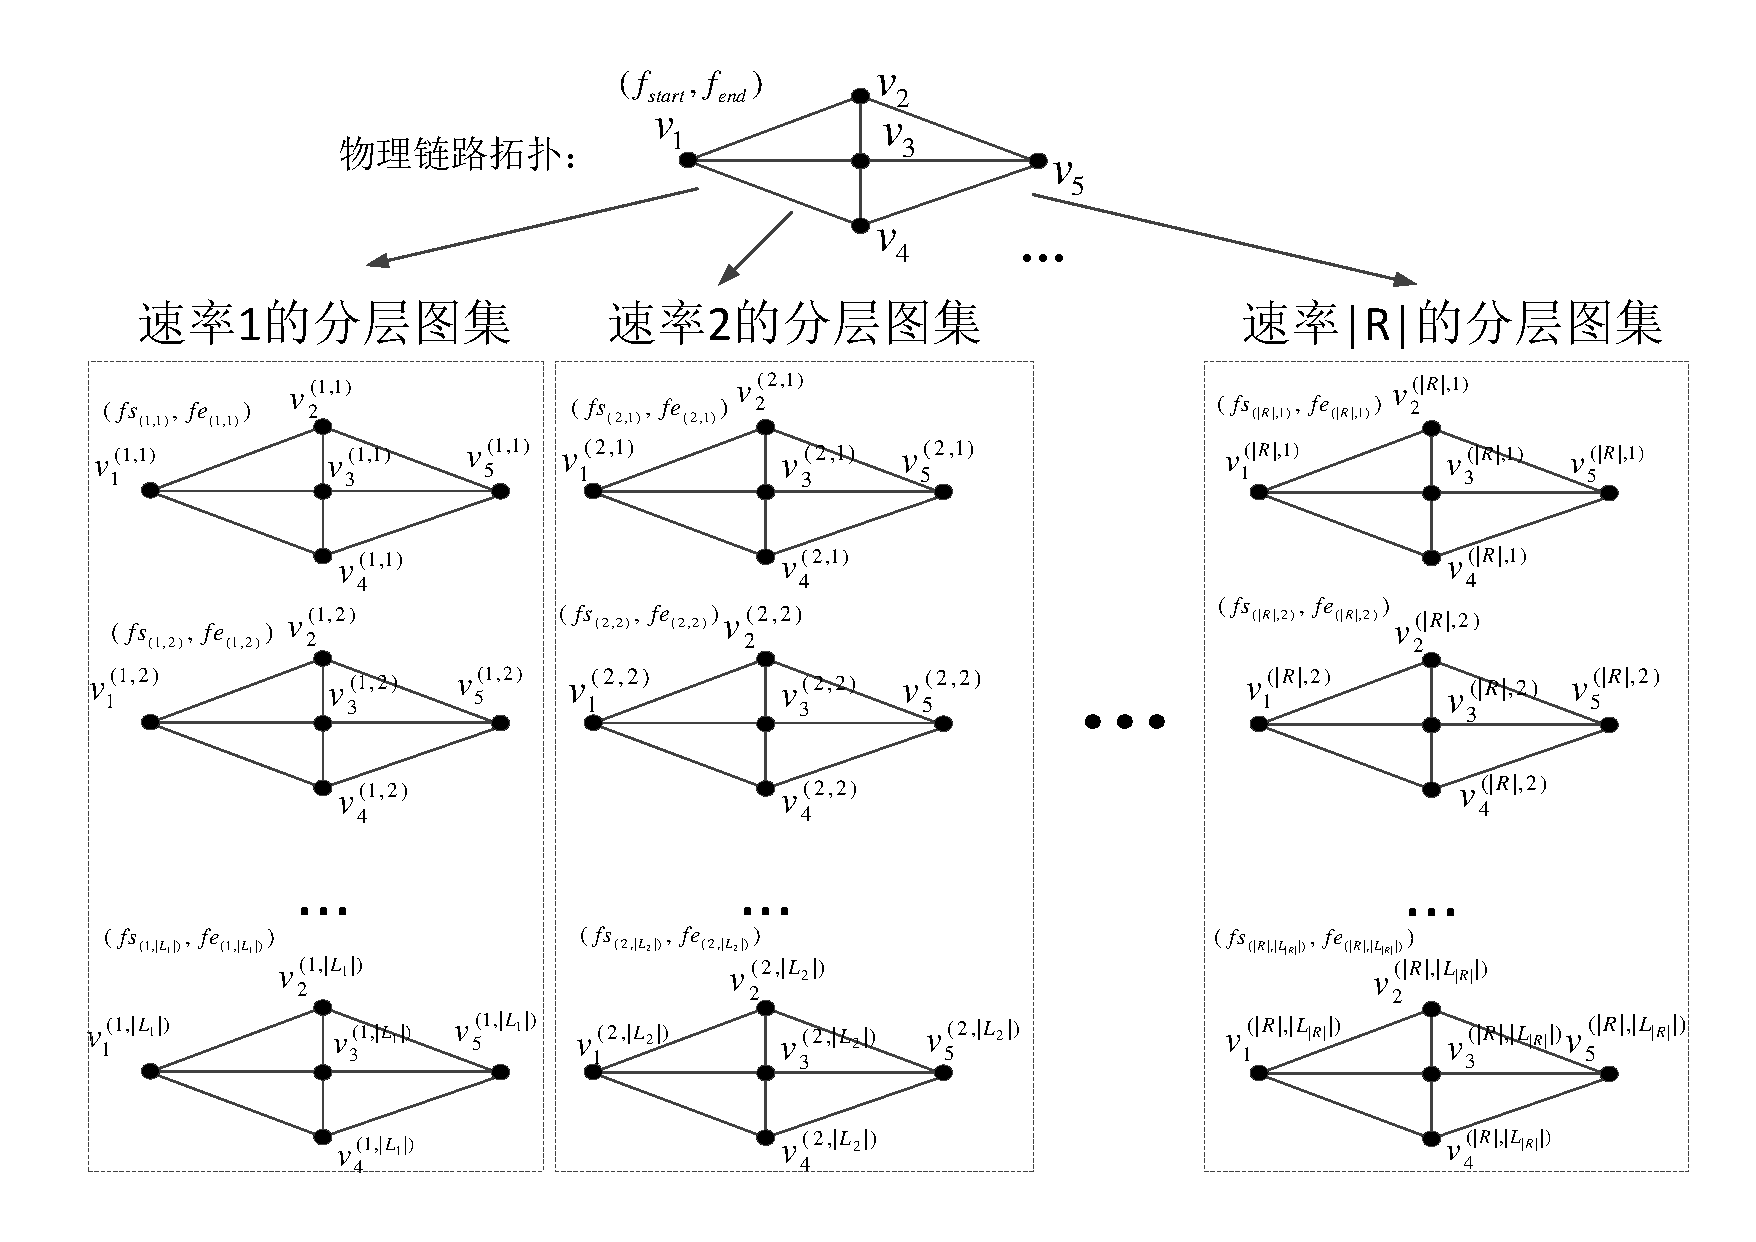
\includegraphics[width=1 \textwidth]{figures/LAYER.pdf}}
\end{center}
\caption{{\footnotesize{分层图组织结构示意}}}
\label{layer}
\end{figure*}
\section{分层图模型下的业务量工程算法}
根据前面的讨论,当一个速率为$r$的业务$TD_r(s,t)$到达网络时,一共有$L_r$ 个分层平面都可以用于此业务,也就是说如果在这些图当中都能为业务找到合适的路径的话,那么业务就有$L_r$ 条路径可供选择,我们可以选择代价最小的一条来优化路由。进一步,当有一批速率为$r$ 的业务集合$D_r$到达网络时,如果大家都选择同一层加入的话,会出现大量的冲突,而且路由代价也会很大,但是现在对每一个业务都有多个分层图平面可以选择,这就给路由代价的优化提供了可能,不同的业务可以选择不同层上的路径来进行路由,以使得总体路由代价减小,节省网络频谱资源,从而优化阻塞率。

根据以上讨论,本节提出一个基于分层图模型的频谱分配与业务量工程算法(TESAA,Traffic Engineering and Spectrum Allocate Algrithm),算法在进行频谱分配的同时对业务的路由代价进行优化,算法流程如图 \ref{bblayer}所示。
\begin{figure*}
\vspace{-1cm}
\setlength{\abovecaptionskip}{-0.5cm}
%\setlength{\belowcaptionskip}{-0.5cm}
\begin{center}
{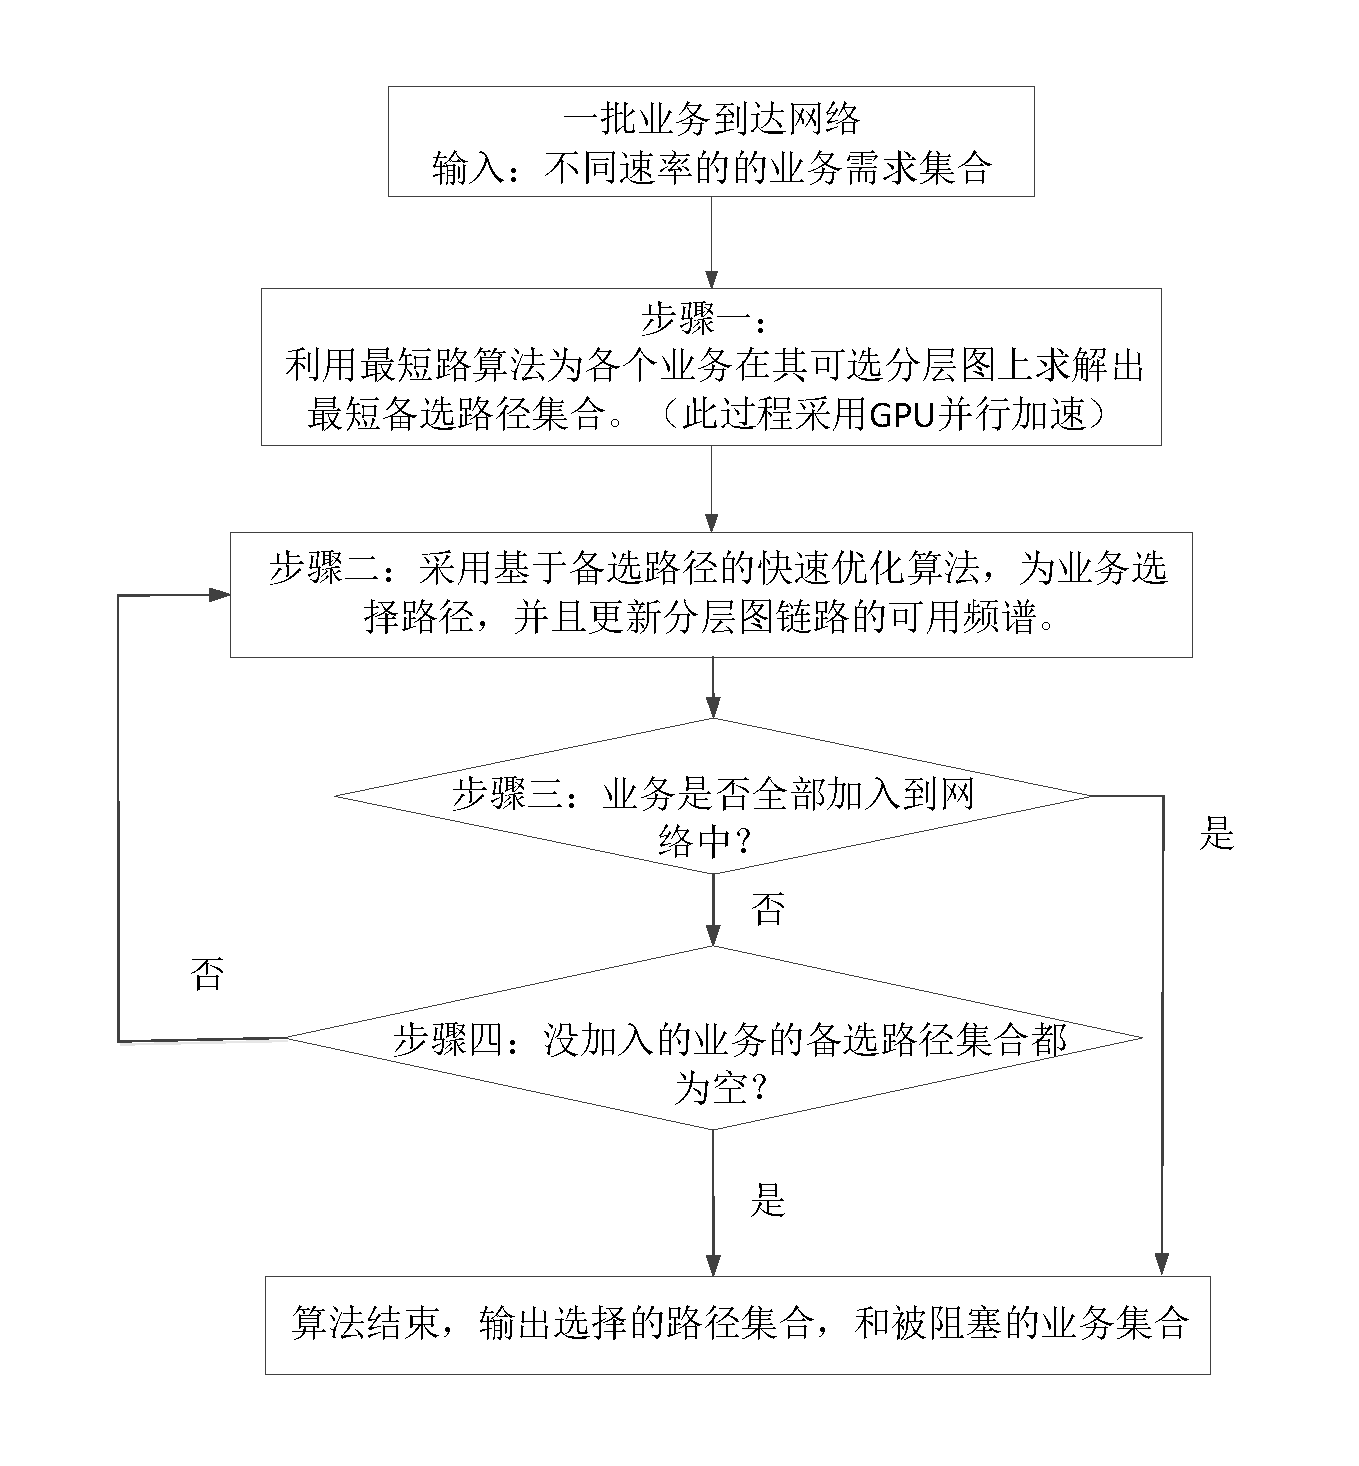
\includegraphics[width=0.9\textwidth]{figures/bbprocess.pdf}}
\end{center}
\caption{{\footnotesize{算法优化流程}}}
\label{bblayer}
\end{figure*}

当一批业务到达网络时,算法会对每一个业务在其所有可用分层图上计算路由,这个过程的计算量较大。但是不同业务之间是独立的,不同分层图之间也是独立的,所以可以采用并行算法来进行加速设计,4.4和4.5将讨论无权图和有权图上的并行路由算法来加速这个步骤。当备选路径都求出来了之后,我们采用一种快速路径选择算法来把业务安排进网络,这个步骤采用一种简单的贪心算法,实验发现这种简单的贪心算法可以很好的优化路径代价。当业务的路径确定后,如果每个业务都能加入到网络,那么本轮算法结束,如果还有剩余的业务没有被安排进网络,需要判断业务的备选路径集合是否为空,如果为空,则说明所有层都不能为业务求出路径,业务将被阻塞。反之,如果业务的备选路径集合不是空,则说明业务是因为和其他业务的路径冲突而导致不能被安排进网络的,分层图中可能还存在其他可用路径,所以需要重新在分层图中计算路径,算法回到步骤二,对这些业务进行重新计算。

步骤一的具体算法将在4.4和4.5介绍,这里介绍步骤二的快速优化算法,快速优化算法的主要思想是在备选路径集合中为每个业务选择路径以使得整体路径代价最小,在动态环境下需要在短时间内安排好路径,所以为了提高计算速度,这里采用一种简单但快速的贪心算法来进行解决,算法如\ref{arrange}所示。
\begin{algorithm}[htb]
\begin{algorithmic}[1]
\Require
$N(v,E)$:分层图;
$P$:备选路径集合;
$D$:业务需求集合;
\Ensure
$AP$:加入业务的路径集合;
\For{$T \in D$}
\State {对$P_T$中的路径按照路径的代价进行降序排序}
\EndFor
\State {对$T$按照$P_T$中的最小路径代价进行排序}
\For{$T \in D$}
\For{$p \in P_T$}
\If{路径$p$所对应分层图上的相应链路没有被占用}
\State{把$p$加入到$AP$中,并更新$p$所对应的分层网络上的链路。}
\State{\bfseries break}
\EndIf
\EndFor
\EndFor
\end{algorithmic}
\caption{路径选择算法}
\label{arrange}
\end{algorithm}

算法开始时对每个业务的备选路径按照其代价进行降序排序,也就是每个业务优先会选择代价较低的备选路径。然后,再对业务按照其最小代价的路径进行排序,这样保证优先考虑代价较小的业务。然后,算法依次加入业务到网络,对每一个业务,遍历其已经排序好的备选路径,如果在对应分层图上路径所包含的链路都是空闲的,则加入业务到网络中,更新分层图上的相应链路为占用状态,把这个路径$p$ 加入到集合$AP$ 中,最后算法输出路径集合$AP$。
\section{无权图情况下的GPU算法设计}

无权图情况下,路由的代价就是路径的跳数,跳数越少说明占用的网络资源越少,尽量优化路径的跳数可以节省网络资源,进一步的降低动态情况下网络的阻塞。无权图情况下的路由算法一般使用BFS (宽度优先搜索)算法进行求解,BFS 算法从离目的节点最近的点开始,一层一层的进行扩展直到找到目的节点,每扩展一层跳数增加一跳,每扩展一层就需要遍历大量的边,这些边的扩展操作是相互独立的,所以为算法提供了并行设计的可能性,在加上不同分层图上的路由计算是相互独立的,所以总体并行粒度是很大的。下面分别对不同并行层次的设计进行讨论。
\subsection {相同速率业务的并行}

如图\ref{bfs}所示,对速率都为$r$的一批业务,算法并行地在每个分层图上进行路由计算,在各个分层图上,具有相同源节点的业务组成业务组,因为他们的路径可以一起计算。对每一个业务组,在GPU 上开辟$|E|$个线程对每一条边进行扩展操作,那么整个过程的的并行粒度为$|L_r|\times|D_r|\times|E|$,其中$|D_r|$为速率为$r$的业务组数量。
\begin{figure*}
\setlength{\abovecaptionskip}{-0.5cm}
%\setlength{\belowcaptionskip}{-0.5cm}
\begin{center}
{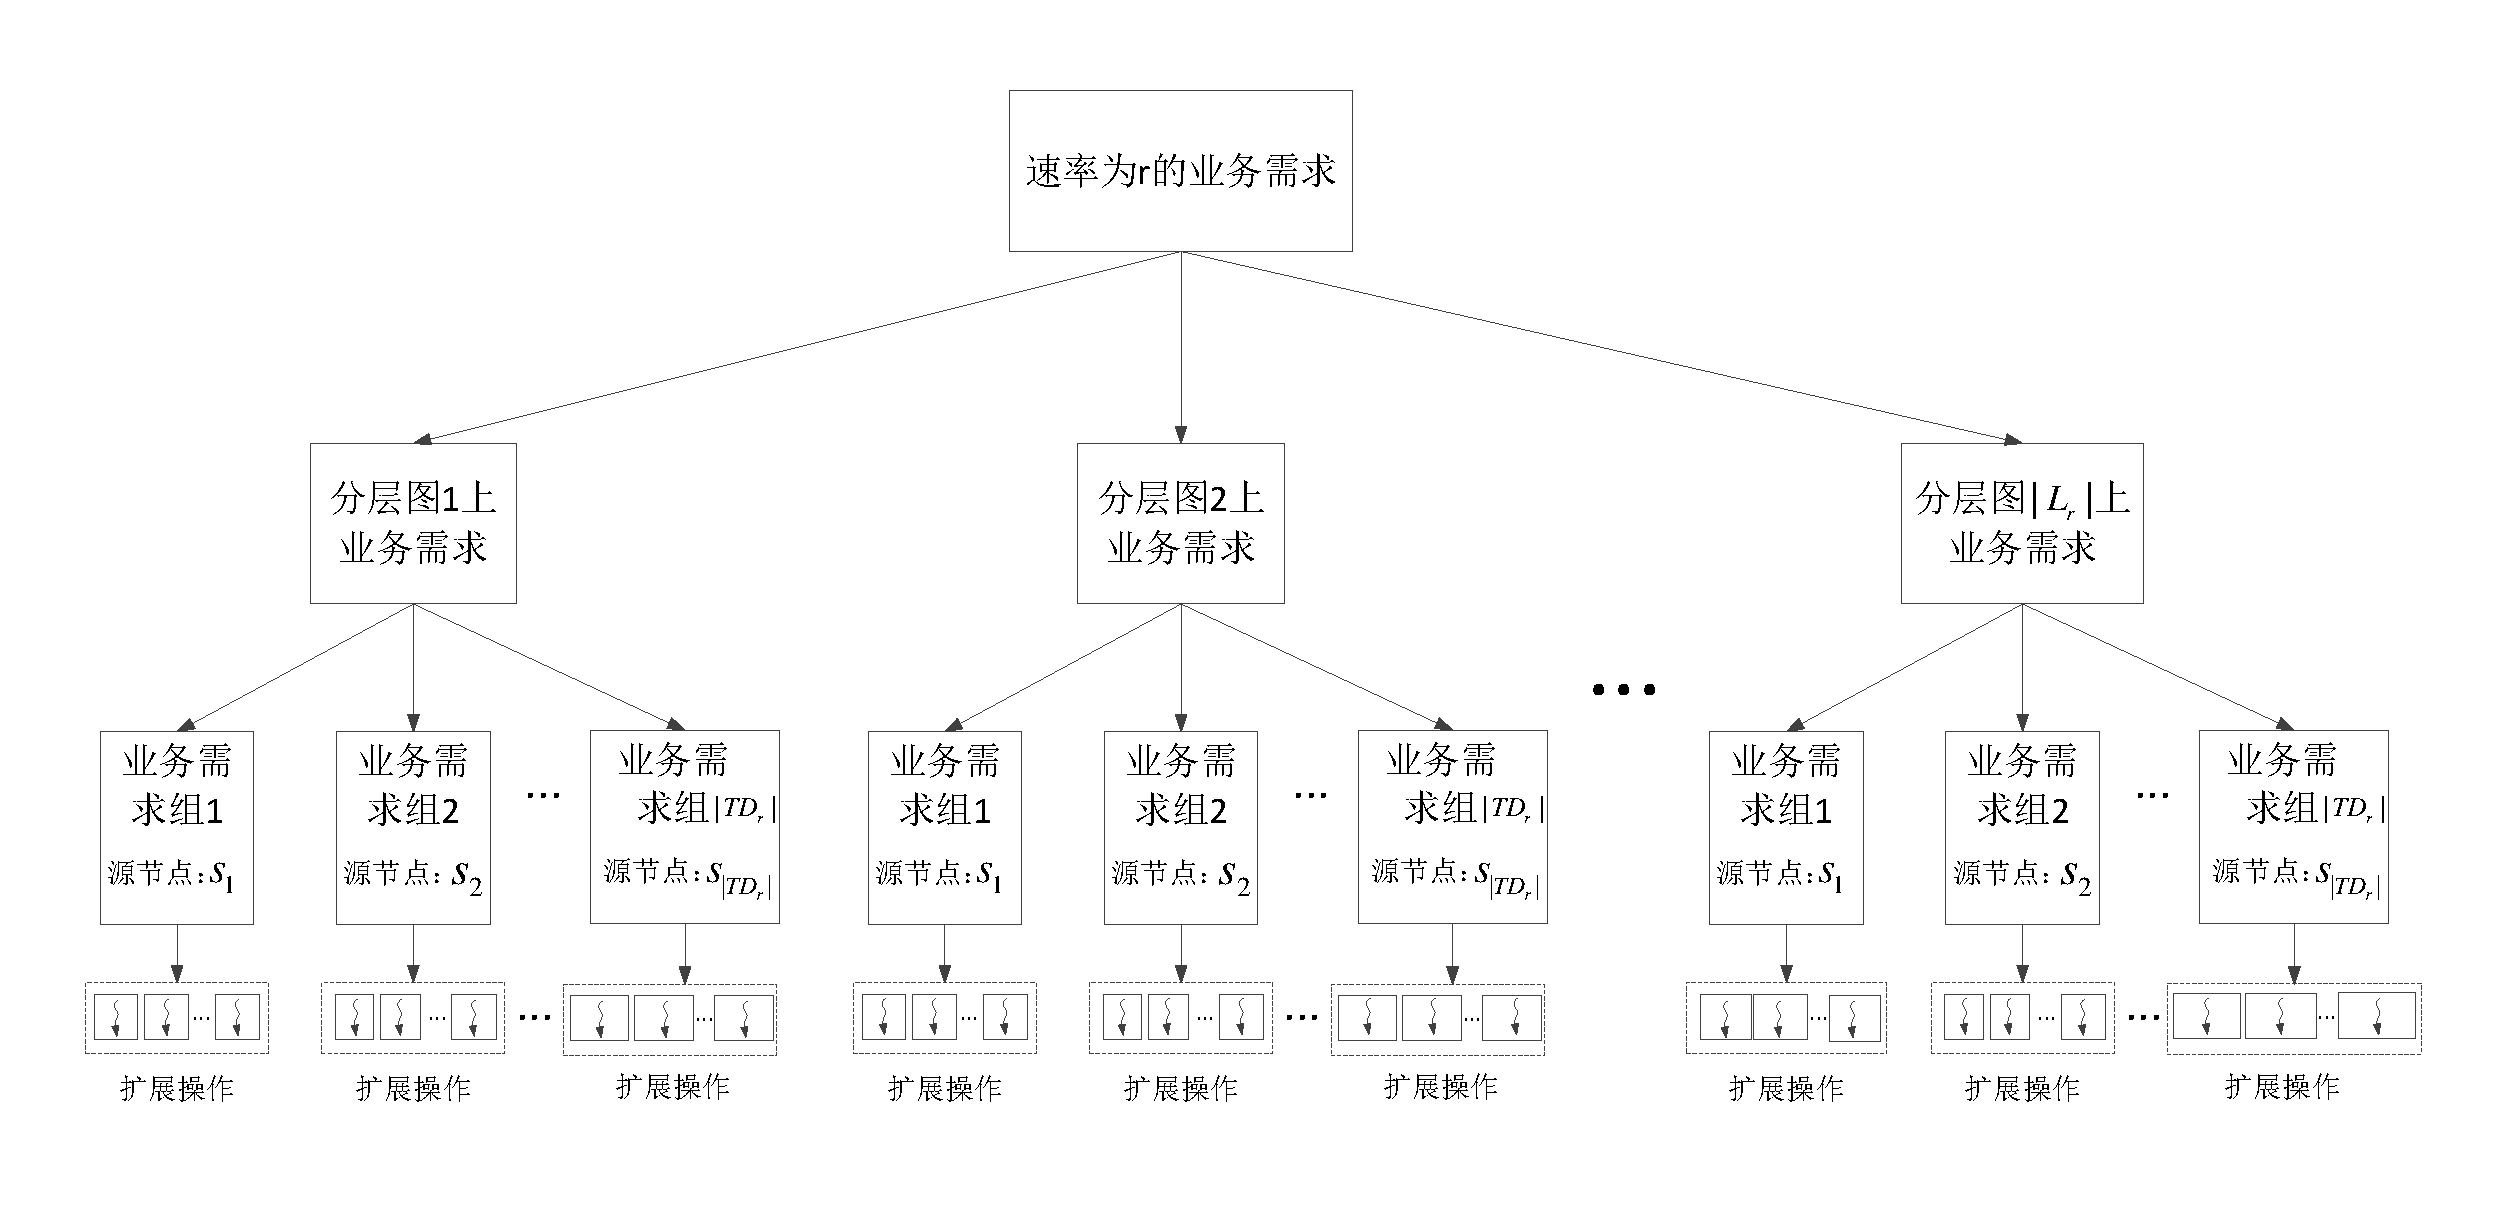
\includegraphics[width=1 \textwidth]{figures/bfs.pdf}}
\end{center}
\caption{{\footnotesize{相同速率业务的BFS并行示意图}}}
\label{bfs}
\end{figure*}
\subsection{不同速率间业务的并行}
由于动态业务情况下每次到达网络的不同数率的业务数量是变化的,不同速率之间业务的并行不容易直接实现在一个kernel中,我们可以把不同速率的业务路由计算抽象成不同的任务,所以本文采用CUDA提供的流并行进行并行设计,如图 \ref{bfssteam}所示。
\begin{figure*}
\setlength{\abovecaptionskip}{-0.5cm}
\begin{center}
{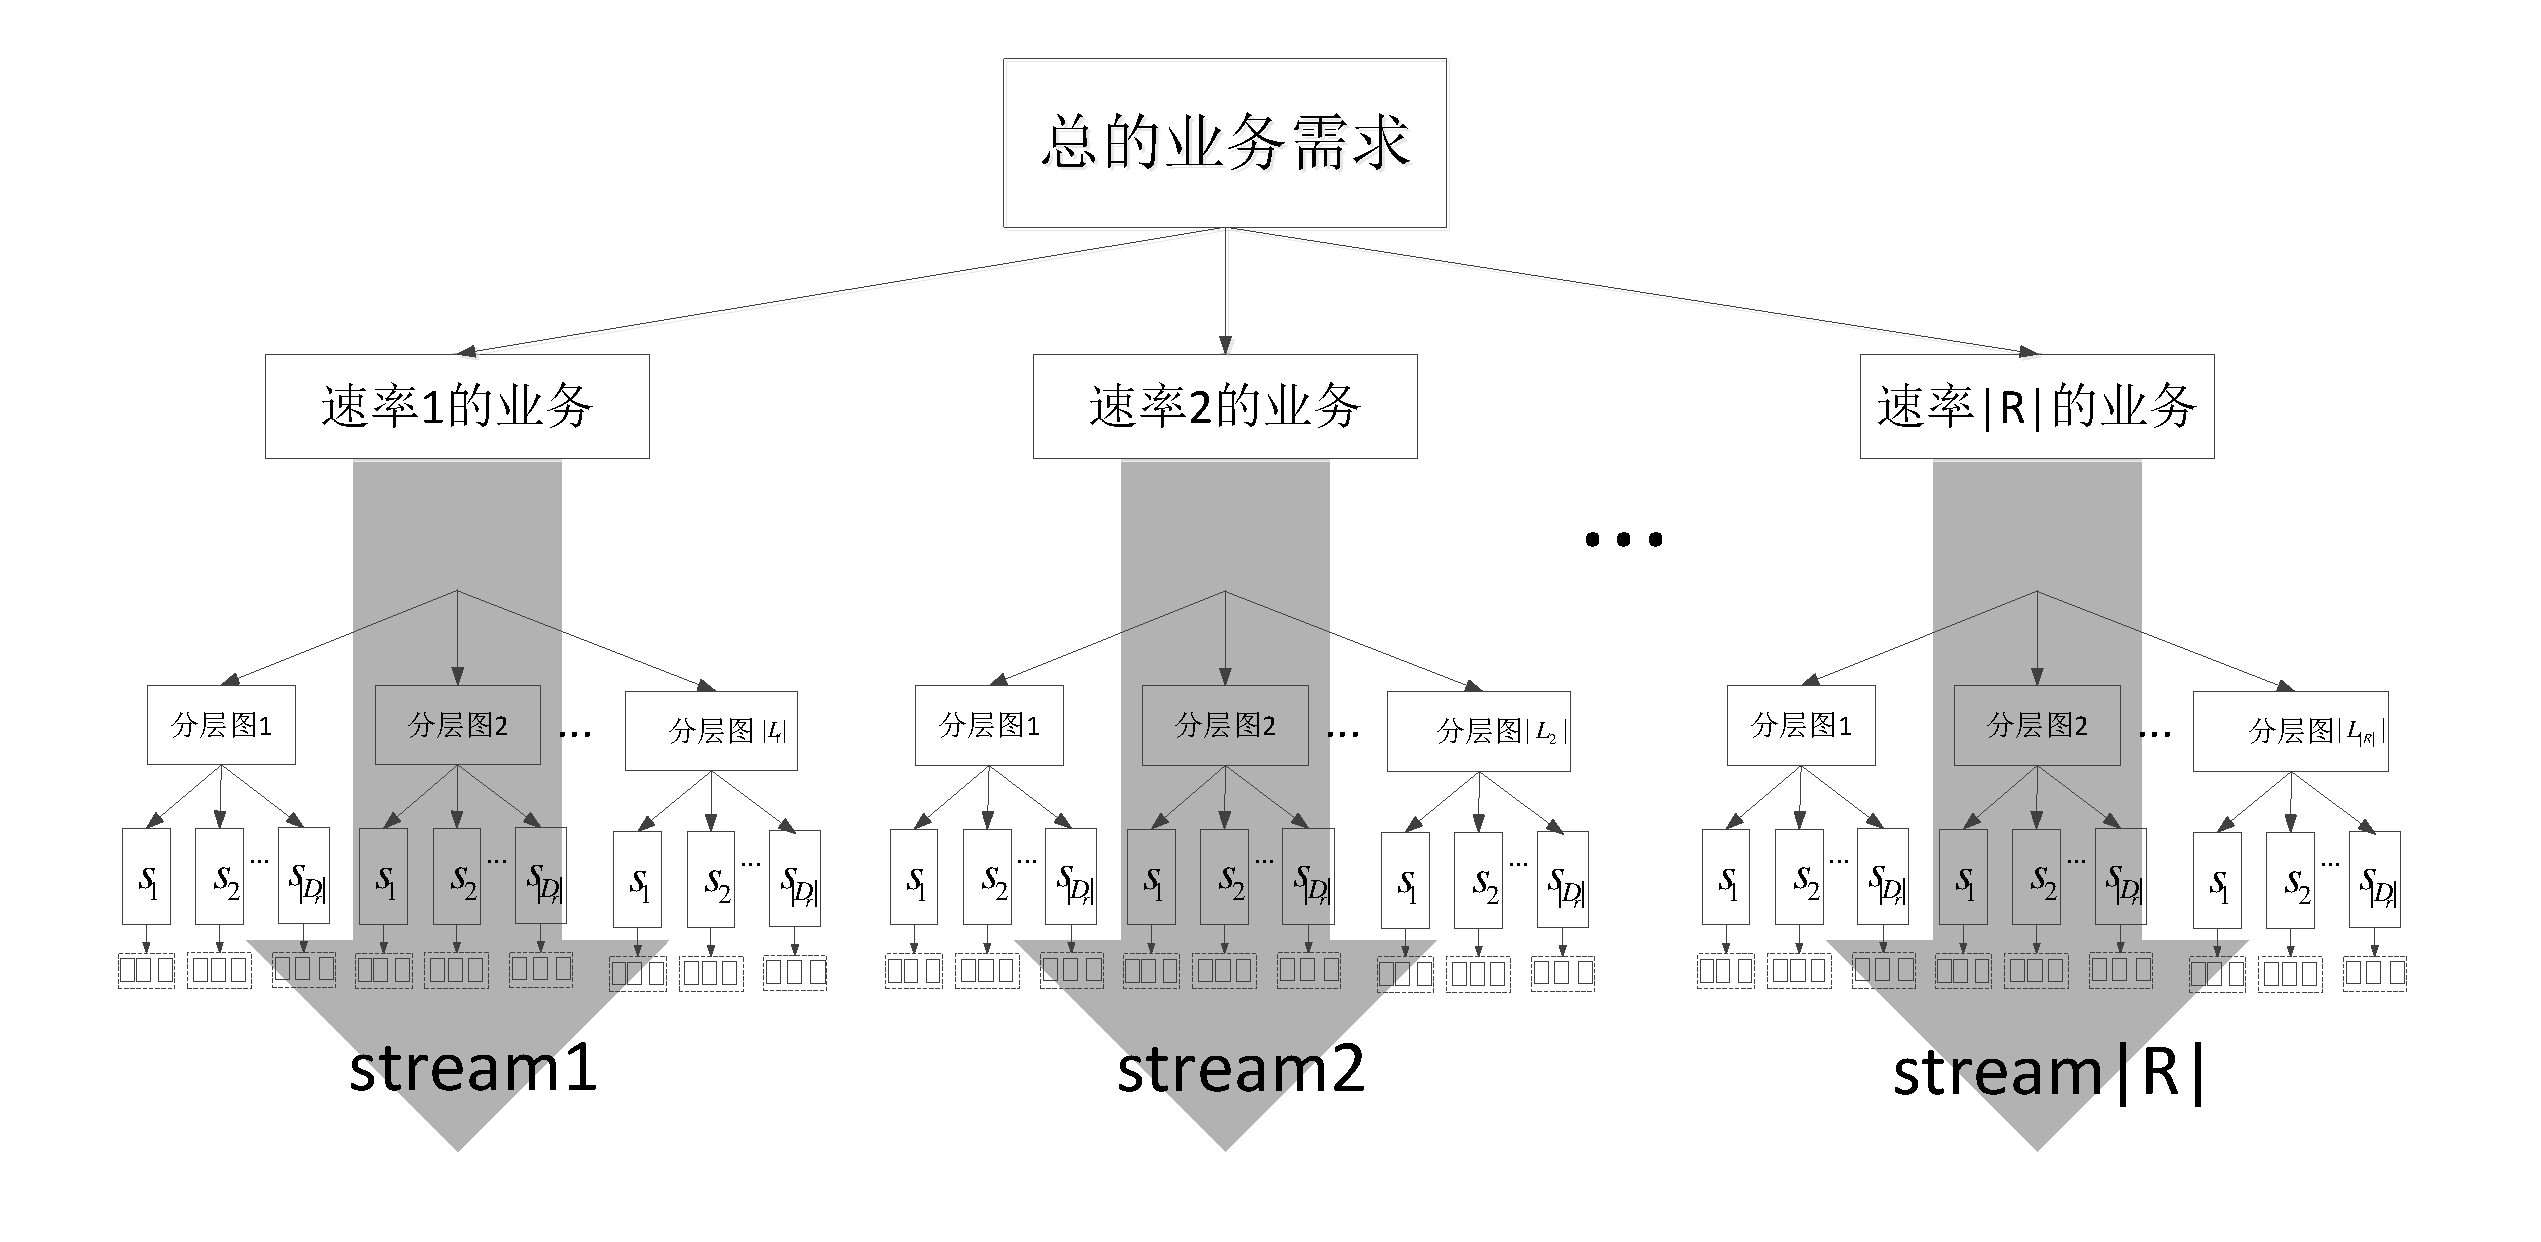
\includegraphics[width=1 \textwidth]{figures/hbfs.pdf}}
\end{center}
\caption{{\footnotesize{BFS流并行示意图}}}
\label{bfssteam}
\end{figure*}

我们为每一个速率建立一个流来负责这个速率的业务计算,假设一共有$|R|$个不同的速率,那么需要建立$|R|$个流,多个流同时切换执行,充分利用GPU的SM资源,当SM资源足够时,不同流的kernel将并行执行,当SM不足时,不同的kernel之间可以进行快速的切换,以达到隐藏延迟的效果。这样,算法的总体并行粒度达到$|L_r|\times|D_r|\times|E|\times|R|$。

\subsection{GPU上的kernel设计}
和3.4.2中讨论的不一样,在BFS的并行中不会存在前驱节点更新的同步问题。但是,我们依然需要两个kernel函数,这是因为扩展操作需要执行多次,如果扩展和更新被放在一个kernel函数,那么更新也会执行多次,这会增加内存的访问,所以我们把两个操作分成两个kernel,一个$kernel\_BFS\_extend$进行边的扩展操作,一个$kernel\_BFS\_update$进行前驱节点的更新操作,其中$kernel\_BFS\_extend$需要多次调用,但是$kernel\_BFS\_update$只需要在最后执行一次。
\begin{algorithm}[t]
\begin{algorithmic}[1]
\Function{kernel\_BFS\_extend}{$E$, $Dist$,$rid$,$round$}
\State {$bid \leftarrow$ block ID}
\State {$tid \leftarrow$ thread ID}
\State {用$(bid,tid,rid)$ 映射到边的标号$eid$}
\State {用$(bid,tid,rid)$ 映射到分层图标号$lid$}
\State {$e \leftarrow E[gid][eid]$}
\If {$e.avaliable==-1$}
\State{return}
\EndIf
\State {用$(bid,tid,rid)$ 映射到的源点标号$sid$}
\If{$Dist[lid][sid][e.head]>round $\&\&$ Dist[lid][sid][e.tail]+1==round$}
\State {$Dist[gid][sid][e.head] \leftarrow round$}
\EndIf
\EndFunction
\end{algorithmic}
\caption{kernel 函数kernel\_BFS\_extend}
\label{Kernelex}
\end{algorithm}

在$kernel\_BFS\_extend$(见算法\ref{Kernelex})中,输入$E$是所有的分层图的边所组成的集合,$Dist$是预先分配的距离标记数组,他是一个三维数组,第一维表示当前距离数组对应的分层图标号,第二维度表示源节点,第三维度表示目的节点,比如$Dist[3][10][5]=4$表示在第3个分层图上,点10到5的距离为4。初始时,除了源节点距离被初始化为0之外,其他的距离都被初始化为无穷大。$rid$表示当前kernel 负责计算的业务速率标号,他是区分不同流的标记,$rid$不同表示执行kernel的流不同。$round$ 表示当前扩展的层数,由于BFS是一层一层地进行扩展操作的,我们需要记录当前层数来决定哪些边需要扩展。算法开始时先进行一系列映射操作,将线程映射到边标号$eid$,当前所在分层图标号$lid$,以及源节点标号$sid$。 由于动态情况下,边的可用状态可能发生变化,找到边之后,需要判断这条边是否可用,如果不可用则返回。接着判断当前边是否可以进行扩展操作,如果尾节点已经更新过了($Dist[lid][sid][e.head] \le round$),则不能再更新了,反之,还需要判断头节点是否是上一次扩展层的节点($Dist[lid][sid][e.tail]+1==round$),如果是的话,那么就更新尾节点的距离为当前扩展层$round$。
\begin{algorithm}[t]
\begin{algorithmic}[1]
\Function{kernel\_bfs\_update}{$E$, $Pre$,$rid$}
\State {$bid \leftarrow$ block ID}
\State {$tid \leftarrow$ thread ID}
\State {用$(bid,tid,rid)$ 映射到边的标号$eid$}
\State {用$(bid,tid,rid)$ 映射到分层图标号$lid$}
\State {$e \leftarrow E[gid][eid]$}
\If {$e.avaliable==-1$}
\State{return}
\EndIf
\State {用$(bid,tid,rid)$ 映射到的源点标号$sid$}
\If{$Dist[lid][sid][e.head]==Dist[lid][sid][e.tail]+1$}
\State {$Pre[gid][sid][e.head] \leftarrow e.tail$}
\EndIf
\EndFunction
\end{algorithmic}
\caption{kernel 函数kernel\_BFS\_update}
\label{KernelBFS}
\end{algorithm}

在$kernel\_BFS\_update$中(见算法\ref{KernelBFS}),其主要逻辑和$kernel\_BFS\_extend$一样,在进行更新判断的时候,判断当前边的头节点是否是尾节点的上一层(Dist[lid][sid][e.head]= Dist[lid][sid][e.tail]+1)如果是的话,那么头节点就有资格作为尾节点的前驱节点,于是进行前驱更新操作。

\begin{algorithm}[t]
\begin{algorithmic}[1]
\Require
业务需求集合$TD$;
分层图链路集合$E$;
\Ensure {业务需求的最短路径集合$P$}
\State {将业务根据速率和源节点重新组合成业务分组集合$D$}
\For {$D_r \in D$}
\For {$d_{rs} \in D_r$}
\For {$l \in L_r$}
\For {$v \in V$}
\If {$v=s$}
\State {$Dist[l][s][v]\leftarrow$ 0}
\Else
\State {$Dist[l][s][v]\leftarrow \infty $}
\EndIf
\State {$Pre[l][s][v]\leftarrow -1 $}
\EndFor
\EndFor
\EndFor
\EndFor
\State {新建$|R|$个流,组成集合$S$}
\State {$round \leftarrow$ 1}
\While{$round \le W_{max}$}
\For{r in R}
\State {在流$S_r$上发射 kernel\_bfs\_extend($E$, $Dist$,$r$,$round$)}
\EndFor
\State{round=round+1}
\EndWhile
\For{r in R}
\State {在流$S_r$上发射 kernel\_bfs\_update($E$, $Dist$,$r$,$round$)}
\EndFor
\State {根据前驱数组$Pre$重建路径,然后把路径加入到集合$P$}
\end{algorithmic}
\caption{{并行BFS计算过程}}
\label{ParaBFS}
\end{algorithm}

介绍完了两个kernel之后,算法 \ref{ParaBFS}展示了整个并行BFS的算法流程,算法 \ref{ParaBFS}开始时先将业务按照速率的不同进行划分,再将业务按照源节点的不同划分成不同的业务组集合,比如,$D_r \in D$表示速率为$r$的业务组集合,$d_{rs} \in D_r$ 表示速率为$r$的源节点标号为$s$的业务组。划分好业务组之后,就开始初始化距离数组,将速率对应的所有分层图上的源节点距离初始化为0,这是一个三层的for 循环,第一层遍历速率标号,第二层遍历源节点标号,第三层遍历速率所对应的分层图标号。初始化$Dist$数组后,在发射kernel之前需要先新建$|R|$个GPU流,不同的流将对不同速率的业务进行计算。$round$ 为扩展的层数标记,开始时$round$初始化为1。while 循环中进行扩展操作,其中$W_{max}$为跳数限制,最大跳数不能超过$W_{max}$,一次扩展操作会使得路径长度增加一跳,所以最多只能循环$W_{max}$次。while循环中for循环用来发射不同的流,因为发射不同流的kernel是异步操作,for循环不会去等待上一个kernel结束了才去执行下一个kernel,所以可以认为所有kernel都是同时间发射的。while循环结束后,算法发射$kernel\_BFS\_update$进行前驱节点记录操作,最后根据这些前驱信息,算法重新恢复出路径,组成路径集合$P$,算法结束。
\section{带权图情况下的GPU算法设计}

在实际应用场景中,我们可能需要将不同的链路设置为不同的代价,所以有必要考虑链路带权情况下的优化设计,算法优化的目标是使得业务的路由代价最小化,在实际应用中很少出现链路代价小于等于零的情况,所以本节假设链路代价均为正值。本节将逐步分析和设计适用于带权图的分层网络GPU并行路由算法。
\subsection{带跳数限制的最短路算法}
带跳数约束的BFS路由,由于没有考虑链路的权重差异,把所有链路的权重看作一样,所以BFS路由的优化目标就是跳数,BFS就是寻找跳数最短的路径,跳数约束只是使得BFS算法提前结束。但是在带权的链路情况下,路由的优化目标是最小化链路代价和,也就是寻找一条代价最小的满足跳数约束的路径,跳数越短并不意味则代价越小,代价越小也不意味着跳数越小,这使得带权情况比无权情况更加复杂。

为了说明带权带跳数约束下的路由算法,我们介绍一些符号,在图$N(V,E)$中,有点$i \in V$和点$j \in V$,假设集合$P_{ijk}$ 表示点$i$到点$j$的所有跳数为$k$的路径所组成的集合,设$p_{ijk}^*$为集合$P_{ijk}$当中代价最小的那一条路径,即$p_{ijk}^* =\arg\min\limits_{p \in P_{ijk}}\{Price\_Of(p)\}$,我们设最小代价数组为$Price$,$Price$为三维数组,其中$Price[i][j][k]=Price\_Of(p_{ijk}^*) )$,即$Price[i][j][k]$表示为$p_{ijk}^*$ 的代价,也就是说$Price[i][j][k]$ 表示$i$ 到$j$ 的跳数为$k$跳的最小代价路径的代价。对点$i$,边集合$PreE_i$表示点$i$ 的入边组成的集合,点集合$PreN_i$表示点$i$的入节点所组成的集合。

有了上面的符号介绍后,假设业务的源节点为$s$,下面给出一个动态规划递推式\ref{dynamic},其中$w_{nj}$ 表示边$(n,j)$ 的代价大小:
\begin{equation}\label{dynamic}
\begin{split}
Price[i][j][k]
=\begin{cases}
\min\limits_{n \in PreN_i}{Price[i][n][k-1]+w_{nj}} & \text{if $k>0$}\\
0 & \text{if $k=0$ and $i=s $} \\
\infty &{otherwise}
\end{cases}
\end{split}
\end{equation}

设$p_{ijk}^*$为点$i$到$j$的跳数为$k$的最小代价路径,由于点$j$的前驱节点只可能是那些属于集合$PreN_j$ 的点,点$j$ 的前驱边只可能是集合$PreE_j$ 中的某一条边,那么最优路径$p_{ijk}^*$中的第$k$条边一定属于集合$PreE_j$,于是递推式中我们遍历了这些边。另外,假设以链路$e$( $e \in PreE_j$)结尾的跳数为$k$的最优路径为$p_{ijk}^e$,那么根据$Price$的定义我们可以得到$Price\_Of(p_{ijk}^e)=Price[i][e.head][k-1]+w_e$,其中,$e.head$表示边的头结点,也就是点$i$的对应于边$e$的前驱节点。那么最优路径$p_{ijk}^*=\arg\min\limits_{e \in PreE_j}{Price\_Of(p_{ijk}^e)}$,相应的最优代价$Price[i][j][k]=\min\limits_{e \in PreE_j}{Price\_Of(p_{ijk}^e)}$,也就是$\min\limits_{n \in PreN_i}{Price[i][n][k-1]+w_{nj}}$。 注意边界情况下($k=0$),由于除了源节点自己之外,源节点到其他节点的跳数不可能是零,所以开始时需要设置代价为无穷大,而源节点到他自己距离设置为0。

上面的动态规划递推式可以求得一个点到任意点的跳数为1到$k$的最优路径,而我们是要求得在跳数限制下的最优代价路径,我们需要对求得的动态规划解进行处理,设二维数组$OPCost$表示跳数限制下的最优路由代价值,那么跳数限制约束下的点$i$到点$j$的最小代价路径的代价为$OPCost[i][j]$,可以得到下面的表达式:
\begin{equation}\label{best}
\begin{split}
OPCost[i][j]=\min\limits_{k \in [1,W_{max}]}{Price[i][j][k]}
\end{split}
\end{equation}

假设满足跳限约束的最优代价路径为$p_{ij}^*$,假设路径$p_{ij}^*$的跳数为$h$,$h \in [1,W_{max}]$,显然$p_{ij}^*=p_{ijh}$,但是实际上我们并不知道$h$ 的值,所以我们从$[1,W_{max}]$ 对$h$进行遍历,那么$p_{ij}^*$肯定是其中代价最小的一条,所以$p_{ij}^*=\arg\min\limits_{k \in [1,W_{max}]}{Price_Of(p_{ijk}^*)}$,同样,$OPCost[i][j]=\min\limits_{k \in [1,W_{max}]}{Price[i][j][k]}$。

\subsection{相同速率业务的动态规划算法并行}

\begin{algorithm}[t]
\begin{algorithmic}[1]
\Require
点的入边集合$PreE$;
点的入点集合$PreN$;
源节点$s$;
\Ensure {最优代价数组$Price$;最优前驱节点数组$Pre$;}
\For {$k \in [1,W_{max}]$}
\For {$v \in V$}
\State {Price[s][v][k]=$\min\limits_{n \in PreN_v}{Price[s][n][k-1]+w_{nv}}$}
\State {Pre[i][j][k]=$\arg\min\limits_{n \in PreN_v}{Price[s][n][k-1]+w_{nv}}$}
\EndFor
\EndFor
\end{algorithmic}
\caption{{串行动态规划算法}}
\label{pda}
\end{algorithm}

上一节我们提出了动态规划模型,证明了算法的正确性,本节我们讨论这个动态规划算法在GPU上的并行算法。

单个图上的动态规划的串行算法如算法\ref{pda}所示,算法循环$W_{max}$次,每一次循环中对每一个点进行$Price$数组的更新,而不同点之间的操作是相互独立的,所以,可以进行并行设计,对每一个点开辟一个线程,每个线程遍历当前点的前驱边,寻找最优的那一条前驱边,并且对$Price$数组进行更新。

相同速率业务间的动态规划并行层次如图\ref{dbs}所示,对速率都为$r$的一批业务,算法并行地在每个分层图上进行路由计算,在各个分层图上,由于源节点相同的业务可以放在一起计算,我们先把业务按照源节点的不同分为一个个的业务组,为每一个业务组开辟$|N|$个线程进行$Price$数组的更新操作,这样总的并行粒度可达到$|N|\times|D|\times|L_r|$。
\begin{figure*}
\setlength{\abovecaptionskip}{-0.5cm}
%\setlength{\belowcaptionskip}{-0.5cm}
\begin{center}
{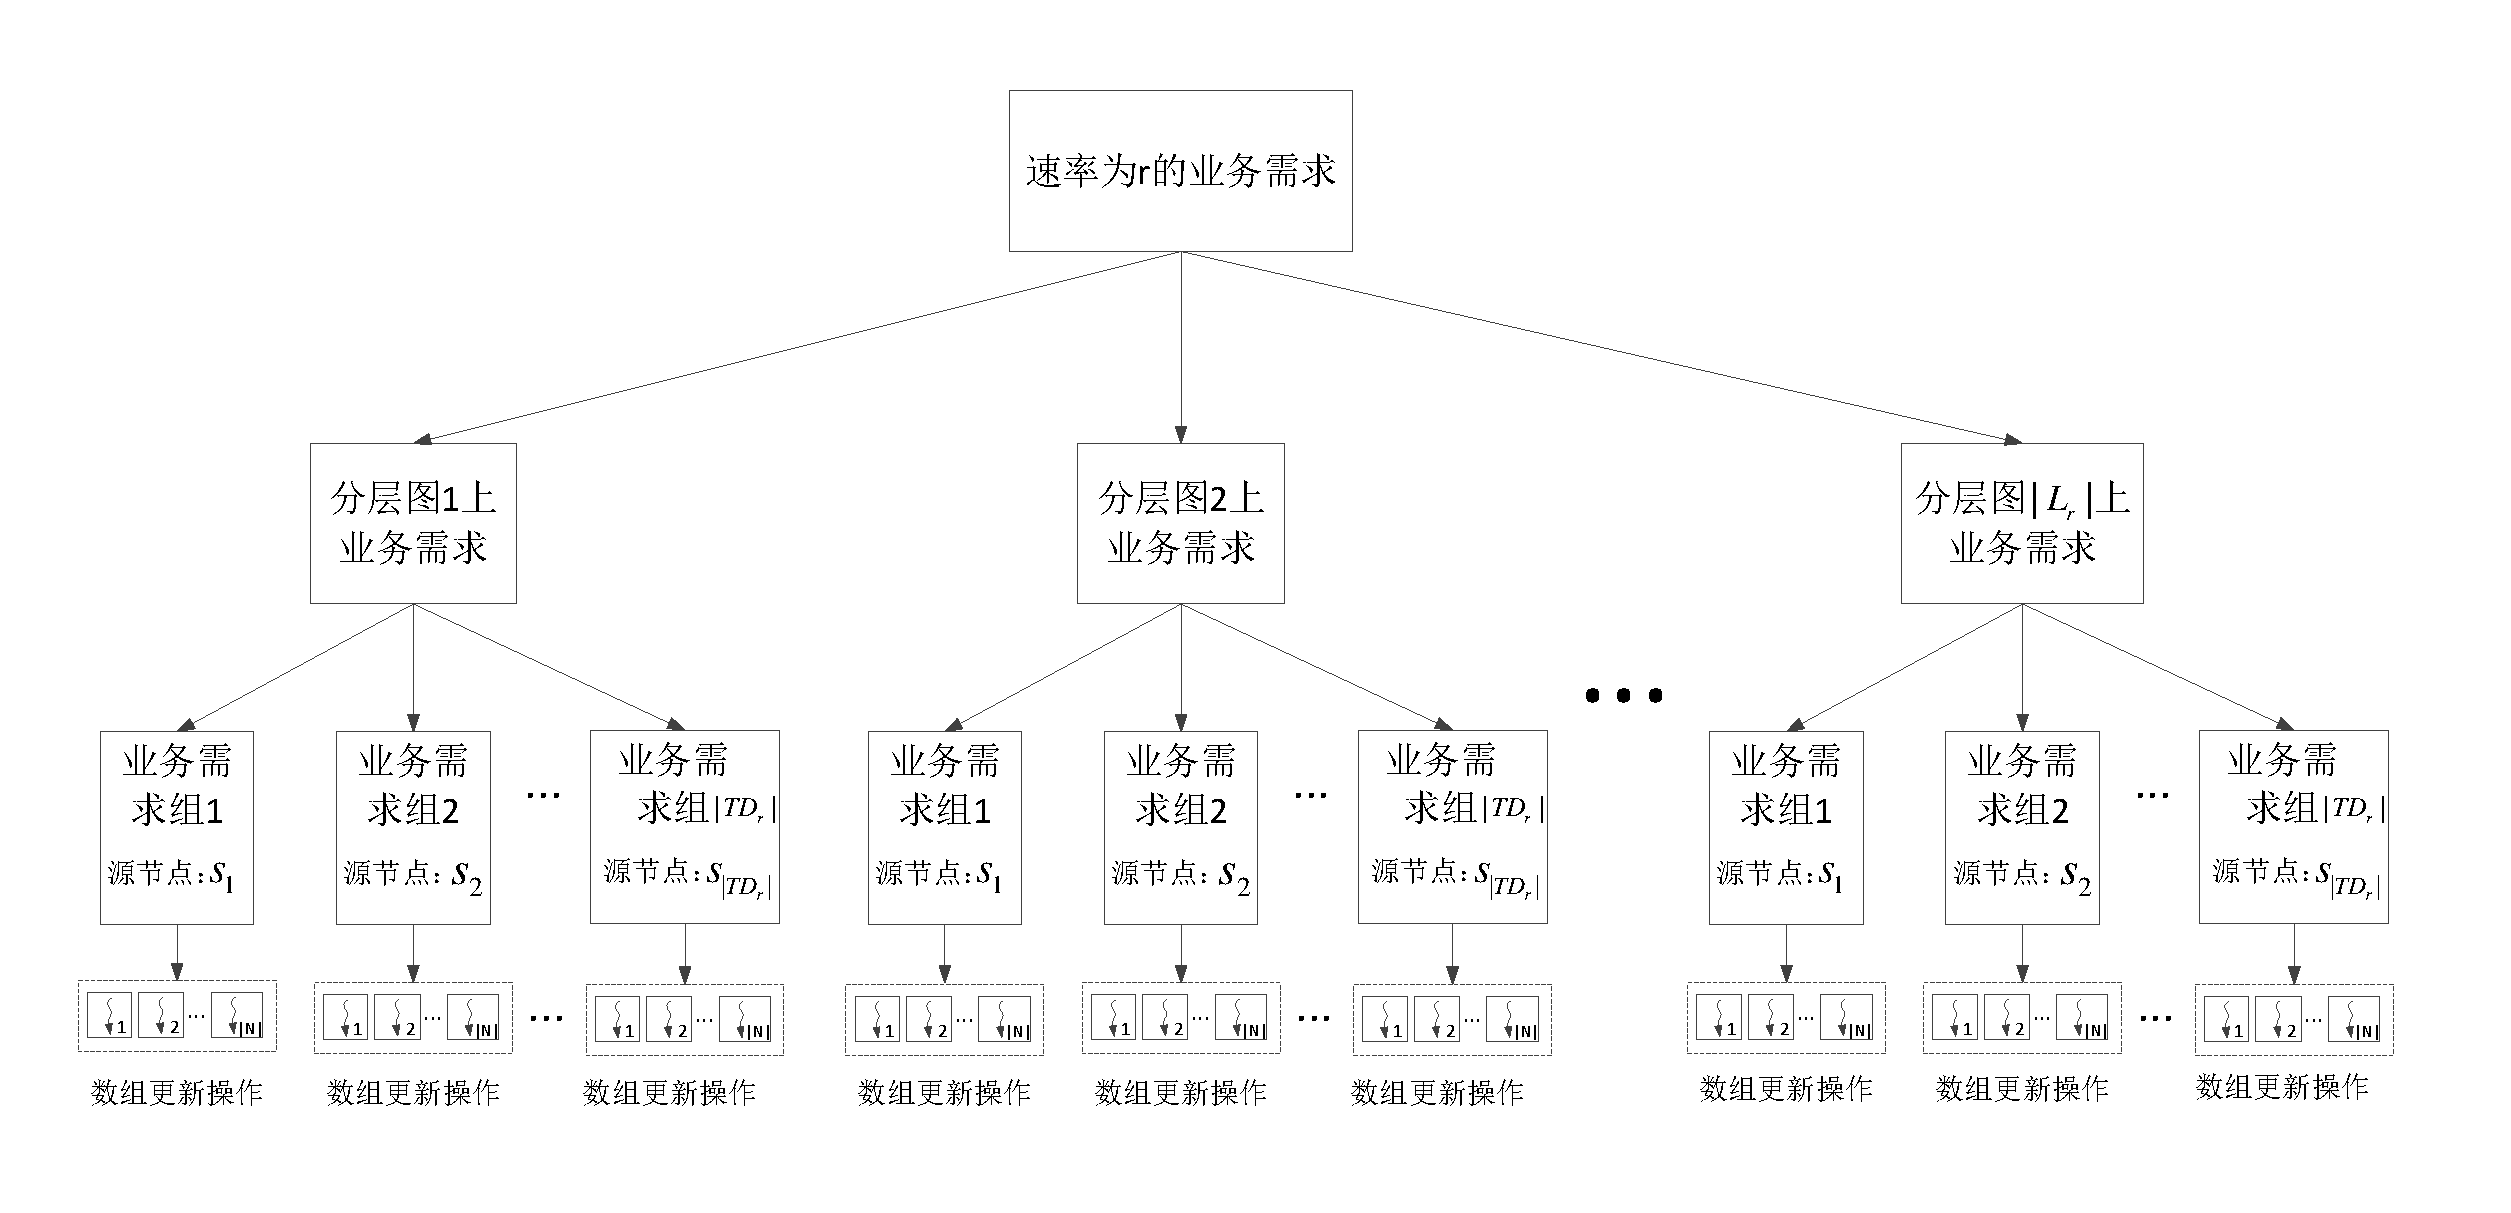
\includegraphics[width=1 \textwidth]{figures/DRK.pdf}}
\end{center}
\caption{{\footnotesize{同速率业务的动态规划并行示意图}}}
\label{dbs}
\end{figure*}
\subsection{不同速率间业务的并行}
和BFS一样,对不同速率的业务,本文依然采用不同的流进行并行,其并行过程如图\ref{BBK}所示。
\begin{figure*}
\setlength{\abovecaptionskip}{-0.5cm}
%\setlength{\belowcaptionskip}{-0.5cm}
\begin{center}
{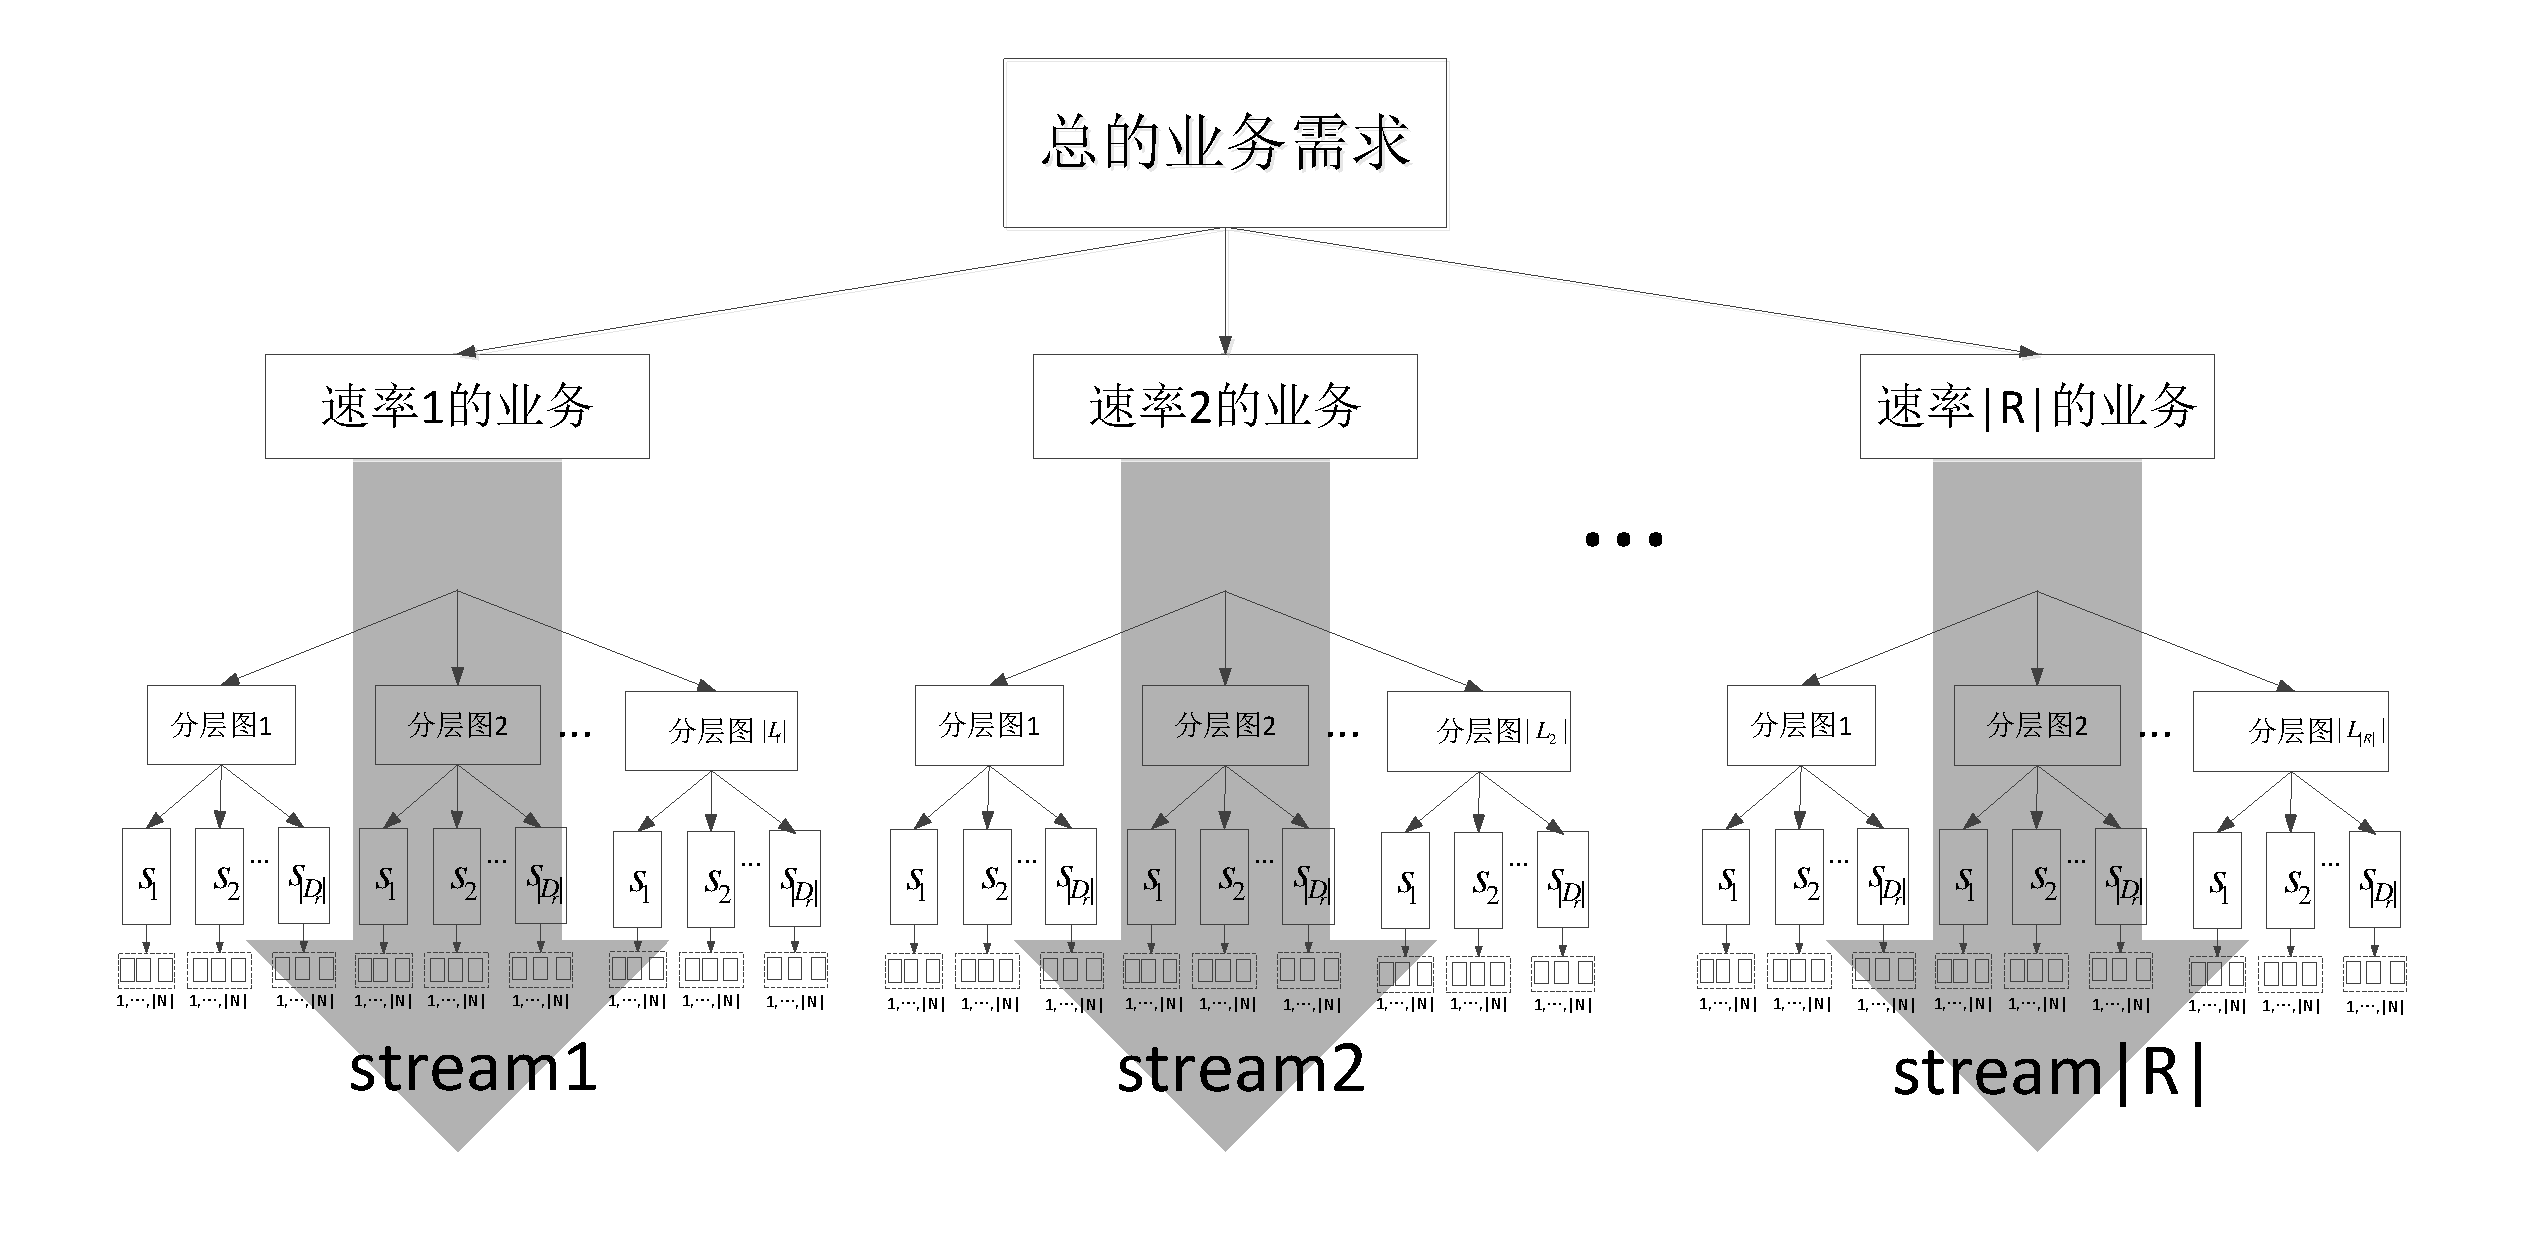
\includegraphics[width=1 \textwidth]{figures/BBK.pdf}}
\end{center}
\caption{{\footnotesize{动态规划流并行示意图}}}
\label{BBK}
\end{figure*}
\subsection{GPU上的kernel设计}
\begin{algorithm}[t]
\begin{algorithmic}[1]
\Function{kernel\_dynamic\_update}{$PE$,$rid$,$k$}
\State {$bid \leftarrow$ block ID}
\State {$tid \leftarrow$ thread ID}
\State {用$(bid,tid,rid)$ 映射到边点的标号$nid$}
\State {用$(bid,tid,rid)$ 映射到边源节点的标号$sid$}
\State {用$(bid,tid,rid)$ 映射到分层图标号$lid$}
\For {$e \in PE[lid][nid]$}
\If{$e.avalible>0$}
\If {$Price[lid][sid][nid][k]<Price[lid][sid][e.s][k-1]+e.weight$}
\State{$Price[lid][sid][nid][k]=Price[lid][sid][e.s][k-1]+e.weight$}
\State{$Pre[lid][sid][nid][k]=e.s$}
\EndIf
\EndIf
\EndFor
\EndFunction
\end{algorithmic}
\caption{kernel\_dynamic\_update}
\label{KernelDynamic}
\end{algorithm}

动态规划的并行算法中我们只需要一个kernel($kernel\_dynamic\_update$),如算法\ref{KernelDynamic}所示,在kernel中,输入$PE$是一个二维的集合数组,比如,$PE[2][3]$表示第2个分层图上点3的入边集合。$Price$ 是预先分配的代价数组,他是一个四维数组,第一维表示当前代价数组对应的分层图标号,第二维度表示源节点,第三维度表示目的节点,第四维度表示路径的跳数,比如$Price[4][3][10][5]$=7 表示在第4个分层图上,点3到点10的跳数为5的最优路径代价为7,初始时,当跳数等于0 时,除了源节点代价被初始化为0之外,其他的距离都被初始化为无穷大。$Pre$数组是前驱数组用以记录前驱信息来恢复路径,$Pre$数组和$Price$数组一样,是一个四维数组,$Pre[4][3][10][5]$=50表示在第4个分层图上,点3到点10的跳数为5的最优路径的前驱节点(也就是路径上的倒数第二个点)为点50。$rid$表示当前kernel 负责计算的业务速率标号,他是区分不同流的标记,$rid$ 不同表示执行kernel的流不同。$k$ 表示当前扩展的层数,也就是跳数。算法开始时先进行一系列映射操作,将线程映射到点标号$eid$,当前所在分层图标号$lid$,以及源节点标号$sid$。映射完成后就可以进行$Price$数组的更新了,也就是要去寻找最优的入边,算法遍历点的所有入边。由于动态情况下,边的可用状态可能发生变化,找到边之后,需要判断这条边是否可用,如果不可用则跳过这条边,反之,就判断更新条件是否成立($Price[lid][sid][nid][k]<Price[lid][sid][e.s][k-1]+e.weight$),如果条件成立则说明这条入边比之前的要好,经过这条边到达当前点的路径代价更小,所以要更新$Price$数组,同时为了后面恢复路径,需要记录前驱信息在数组$Pre$中。
\begin{algorithm}[t]
\begin{algorithmic}[1]
\Require
业务需求集合$TD$;
各个分层图前驱链路集合$PE$;
\Ensure {业务需求的最短路径集合$P$}
\State {将业务根据速率和源节点重新组合成业务分组集合$D$}
\For {$D_r \in D$}
\For {$d_{rs} \in D_r$}
\For {$l \in L_r$}
\For {$v \in V$}
\If {$v==s$}
\State {$Price[l][s][v][0]\leftarrow$ 0}
\Else
\State {$Price[l][s][v][0]\leftarrow \infty $}
\EndIf
\State {$Pre[l][s][v][0]\leftarrow -1 $}
\EndFor
\EndFor
\EndFor
\EndFor
\State {新建$|R|$个流,组成集合$S$}
\State {$k \leftarrow$ 1}
\While{$k<=W_{max}$}
\For{r in R}
\State {在流$S_r$上发射 kernel\_dynamic\_update($PE$,$rid$,$k$)}
\EndFor
\State{$k=k+1$}
\EndWhile
\State {根据前驱数组$Pre$重建路径,然后把路径加入到集合$P$}
\end{algorithmic}
\caption{{并行动态规划的计算}}
\label{Parad}
\end{algorithm}

算法\ref{Parad}展示了整个动态规划的计算过程,算法开始时先将业务按照速率的不同进行划分,再将业务按照源节点的不同划分成不同的业务组集合$D$,比如,$D_r \in D$表示速率为$r$ 的业务组集合,$d_{rs} \in D_r$ 表示速率为$r$的源节点标号为$s$的业务组。划分好业务组之后,就开始初始化代价数组,将速率对应的所有分层图上的跳数为0的源节点代价初始化为0,这是一个三层的for循环,第一层遍历速率标号,第二层遍历源节点标号,第三层遍历速率所对应的分层图标号。初始化$Price$数组后,在发射kernel之前需要先新建$|R|$ 个GPU 流,不同的流将对不同速率的业务进行计算。$k$为扩展的跳数标记,开始时$k$初始化为1。while循环中进行扩展操作,其中$W_{max}$为跳数限制,最大跳数不能超过$W_{max}$,所以最多只能循环$W_{max}$次。while循环中for循环用来发射不同的流,因为发射不同流的kernel 是异步操作,for循环不会去等待上一个kernel结束了才去执行下一个kernel,所以可以认为所有kernel都是同时间发射的。
\section{实验仿真分析}
\subsection{对比算法}
为了说明TESAA对路径代价和网络阻塞率带来的优化效果,我们将PTESAA/STESAA和不进行路由代价优化的贪心算法进行比较,我们称这个算法为GRSAA(Greedy Routing and Spectrum Allocation Algorithm),如算法\ref{ParaSPC}所示。当业务到达时,GRSAA先在第一层对所有业务求最短路径,为每个业务估计一个路径跳数值,按照这个跳数值对业务进行排序,这是为了优先加入较短的业务。然后,算法逐层去寻找是否能够把业务加入到网络中,如果能加入到当前层中,那么就更新当前层上的相应链路的占用情况,反之,就在下一层进行搜寻。如果所有层都无法加入这个业务,那么业务就被阻塞,业务被加入到阻塞集合。
\begin{algorithm}[t]
\begin{algorithmic}[1]
\Require
业务需求集合$TD$;
分层图集合$G$;
\Ensure {业务需求的路径集合$P$;阻塞的需求集合$Z$}
\For{$r \in R$}
\State{$flag \leftarrow 0$ }
\For{$D_r \in D$}
\State{把$D_r$中的业务按照其在第一层分层图上的最短路径跳数进行排序}
\For{$d \in D_r$}
\For{$g \in G_r$}
\If{在分层图g上存在业务$d$的合法路径$p$}
\State{更新分层图g上的链路占用情况}
\State{把路径p加入到结果路径集合$P$中}
\State{$flag \leftarrow 1$}
\State{\bfseries break}
\EndIf
\EndFor
\If{$flag=0$}
\State{把业务$d$加入阻塞集合$Z$中}
\EndIf
\EndFor
\EndFor
\EndFor
\end{algorithmic}
\caption{{贪心的分层RSA算法}}
\label{ParaSPC}
\end{algorithm}
\subsection{实验设置}
在本文的实验仿真中,网络的节点数为$N=100$,平均度数为$4$,业务的路径限制$W_{max}=8$。我们假设只存在两种速率的业务,并且已知两种速率的业务的大致比例为1:3。我们初始时为速率1的业务分配20层的频谱连续分层网络,为速率2的业务分配60层的频谱连续的分层网络。我们假设业务的到达服从泊松过程,一共产生了1000个到达事件,每两个连续的到达事件之间的时间间隔服从均值为4的负指数分布,当到达事件发生时,实验产生速率1的业务为$d_1$ 个,产生速率为2的业务$d_2$ 个,其中$d1$ 为$2 \cdot |N|$到$4 \cdot|N|$中的随机值,$d_2$为$6 \cdot |N|$到$12 \cdot |N|$之间的随机值。假设每个业务的服务时间满足均值为$ST$的负指数分布,我们观察各种算法在不同平均服务时间$ST$下的优化情况。

\subsection{无权图下的仿真结果}
\subsubsection{路由跳数优化结果分析}

在无权图中,TESAA的优化目标是最小化路由的跳数,图\ref{B5H}到图\ref{B40H}表示了无权图下跳数的优化结果,我们把PTESAA和STESAA与贪心算法GRSAA进行比较。图中的横坐标表示业务到达的次数,图中的纵坐标表示业务的平均路由跳数。

当网络状况较好的时候,比如,平均服务时间为$ST=5$时,PTESAA/STESAA计算得到的路由平均跳数为2.73,而GRSAA计算得到的路由平均跳数为3.73,PTESAA/STESAA得到的路由平均跳数要比GRSAA得到的路由平均跳数少一跳左右。随着平均服务时间$ST$的增加,PTESAA/STESAA和GRSAA所计算出的路由平均跳数都有所增加,但是PTESAA/STESAA的增幅较小,从$ST=5$时的平均2.73增加到$ST=40$时的平均2.82,而GRSAA的平均路由跳数随着$ST$的增加而大幅增加,从$ST=5$ 时的平均3.75增加到$ST=40$时的平均4.2,可见不管在网络空闲还是网络繁忙的情况下PTESAA都能很好地优化业务路由的跳数,减小对网络资源的占用。
\begin{figure*}
\setlength{\abovecaptionskip}{-0.5cm}
%\setlength{\belowcaptionskip}{-1cm}
\begin{center}
{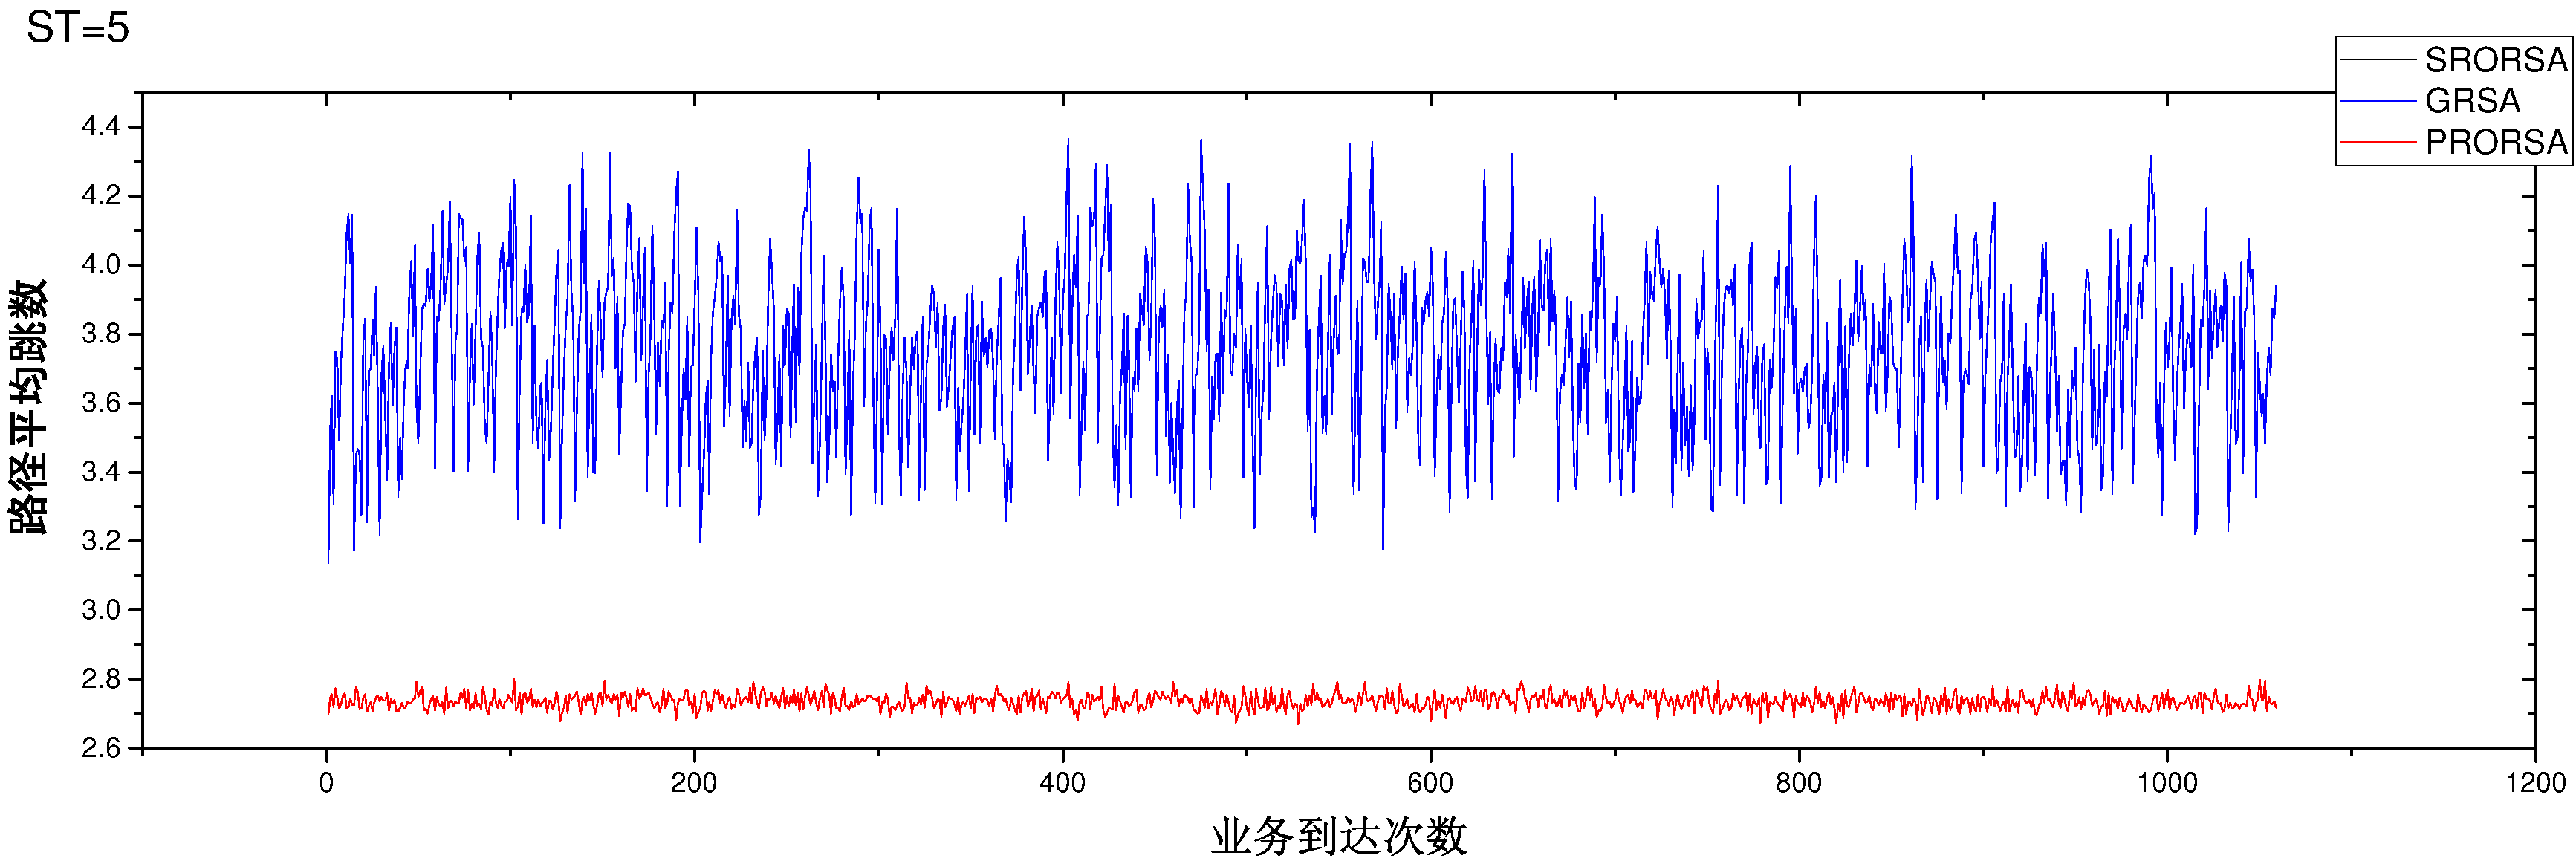
\includegraphics[width=1 \textwidth]{figures/B5H.pdf}}
\end{center}
\caption{{\footnotesize{无权图路径跳数对比(ST=5)}}}
\label{B5H}
\end{figure*}
\begin{figure*}
\vspace{-0.5cm}
\setlength{\abovecaptionskip}{-0.5cm}
%\setlength{\belowcaptionskip}{-1cm}
\begin{center}
{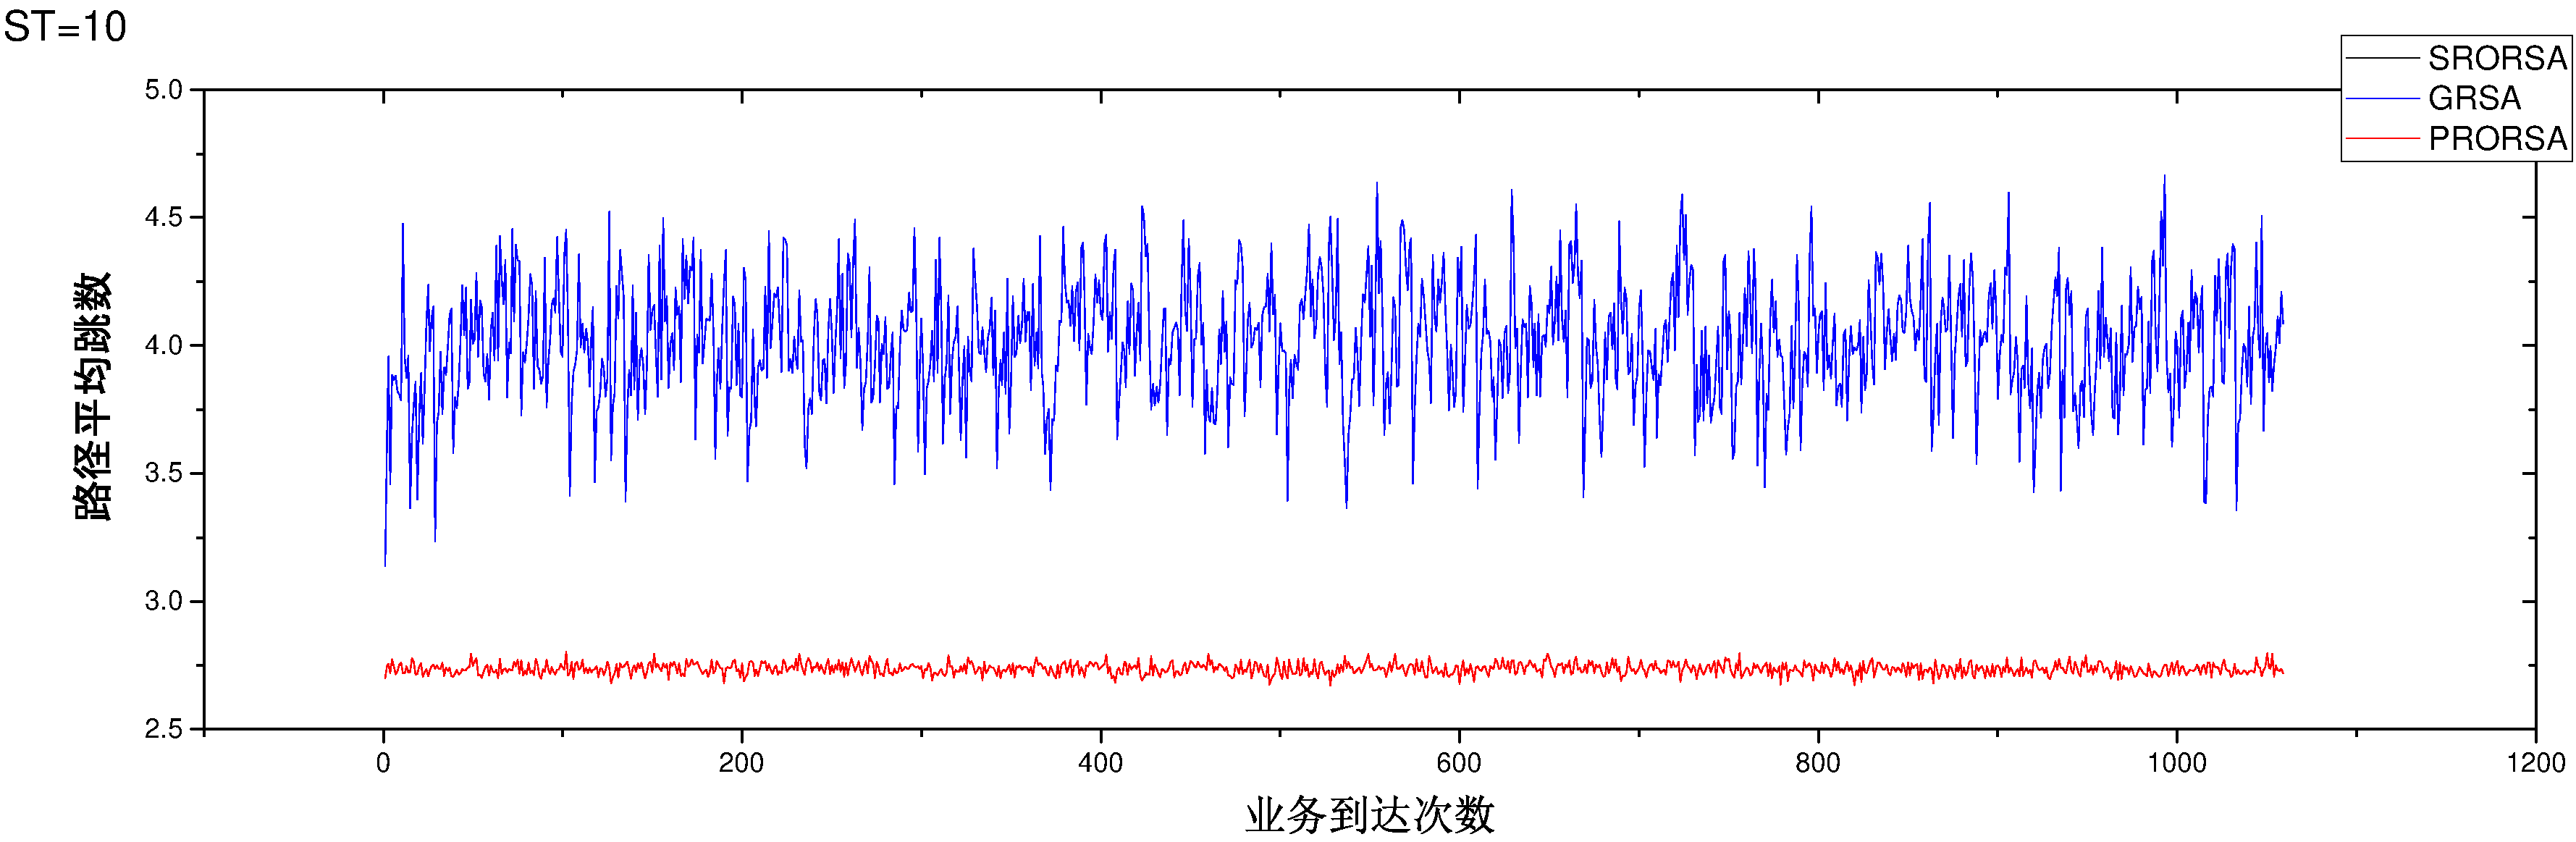
\includegraphics[width=1 \textwidth]{figures/B10H.pdf}}
\end{center}
\caption{{\footnotesize{无权图路径跳数对比(ST=10)}}}
\label{B10H}
\end{figure*}
\begin{figure*}
\vspace{-0.5cm}
\setlength{\abovecaptionskip}{-0.5cm}
%\setlength{\belowcaptionskip}{-1cm}
\begin{center}
{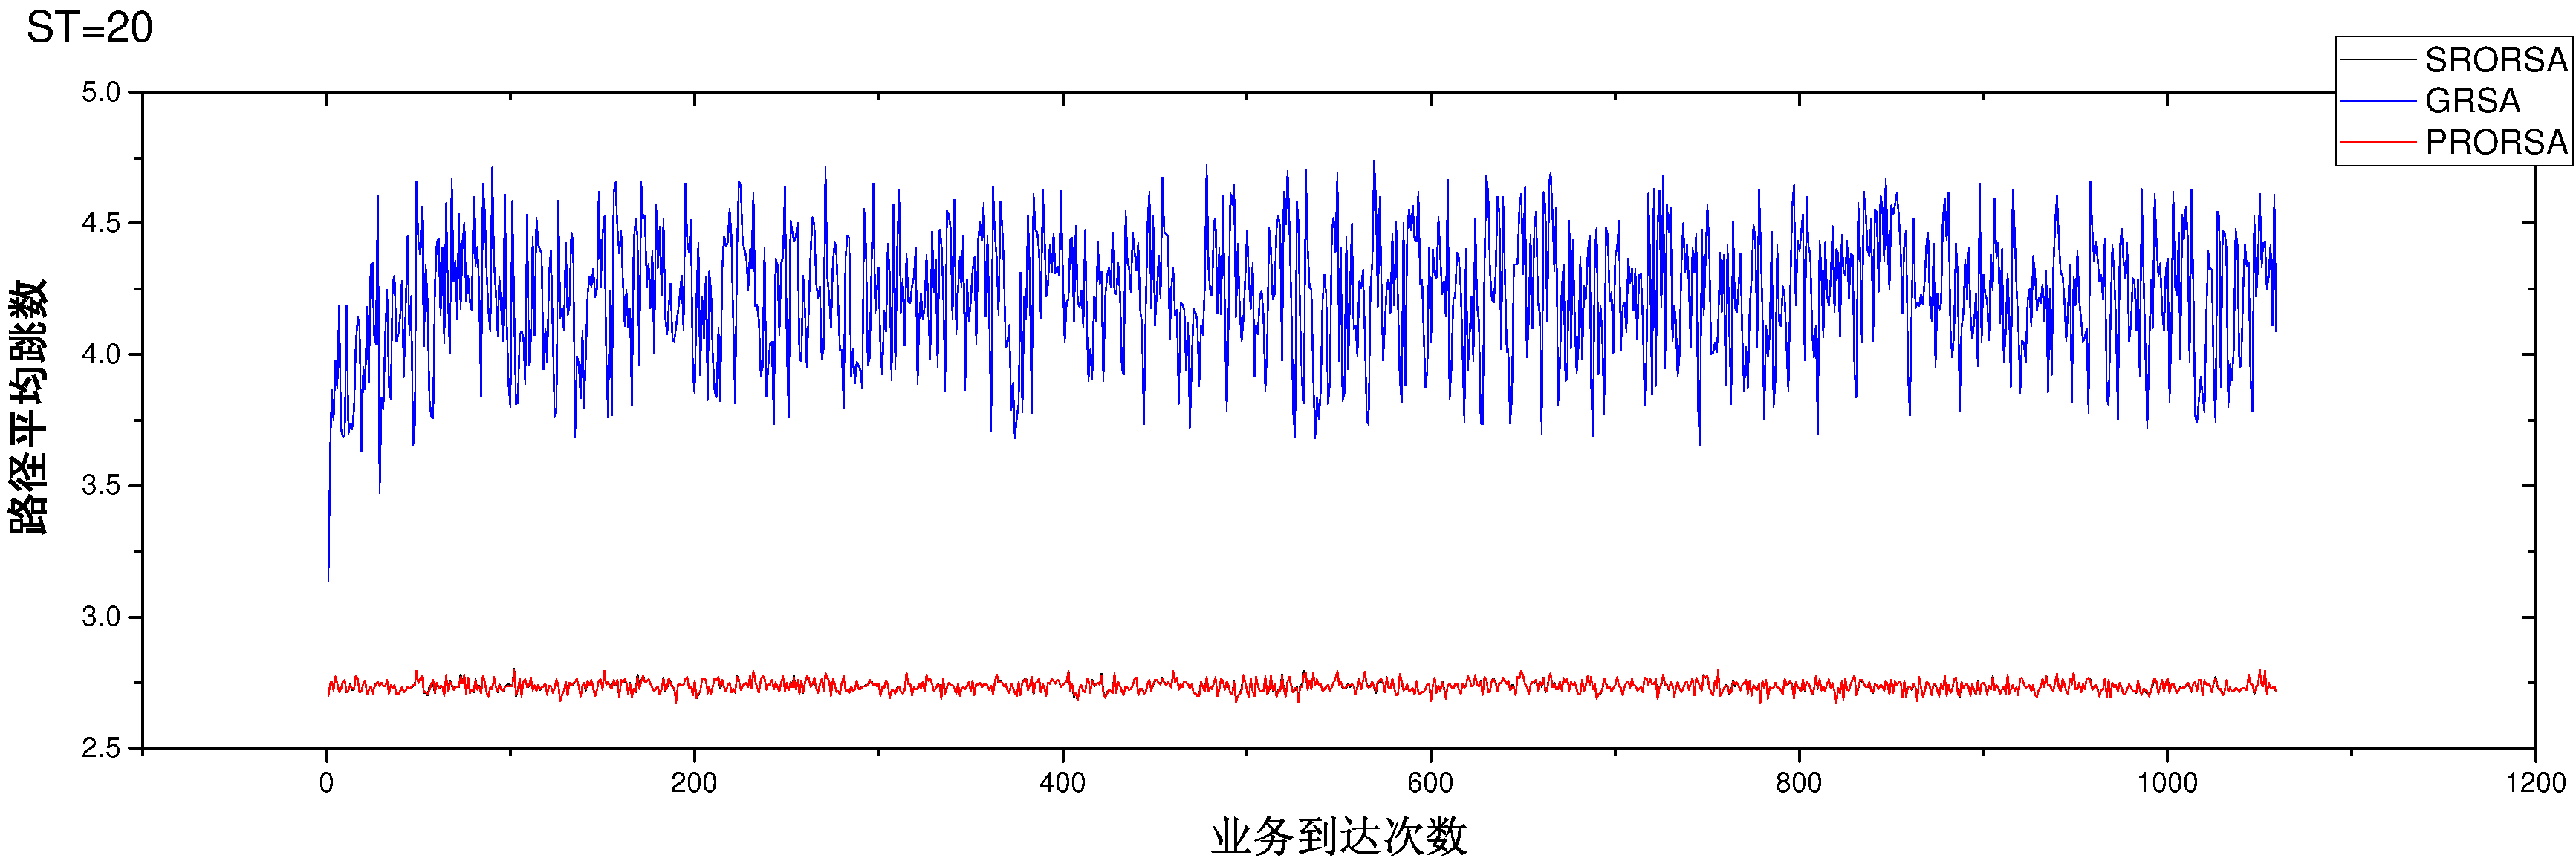
\includegraphics[width=1 \textwidth]{figures/B20H.pdf}}
\end{center}
\caption{{\footnotesize{无权图路径跳数对比(ST=20)}}}
\label{B20H}
\end{figure*}
\begin{figure*}
\vspace{-0.5cm}
\setlength{\abovecaptionskip}{-0.5cm}
%\setlength{\belowcaptionskip}{-1cm}
\begin{center}
{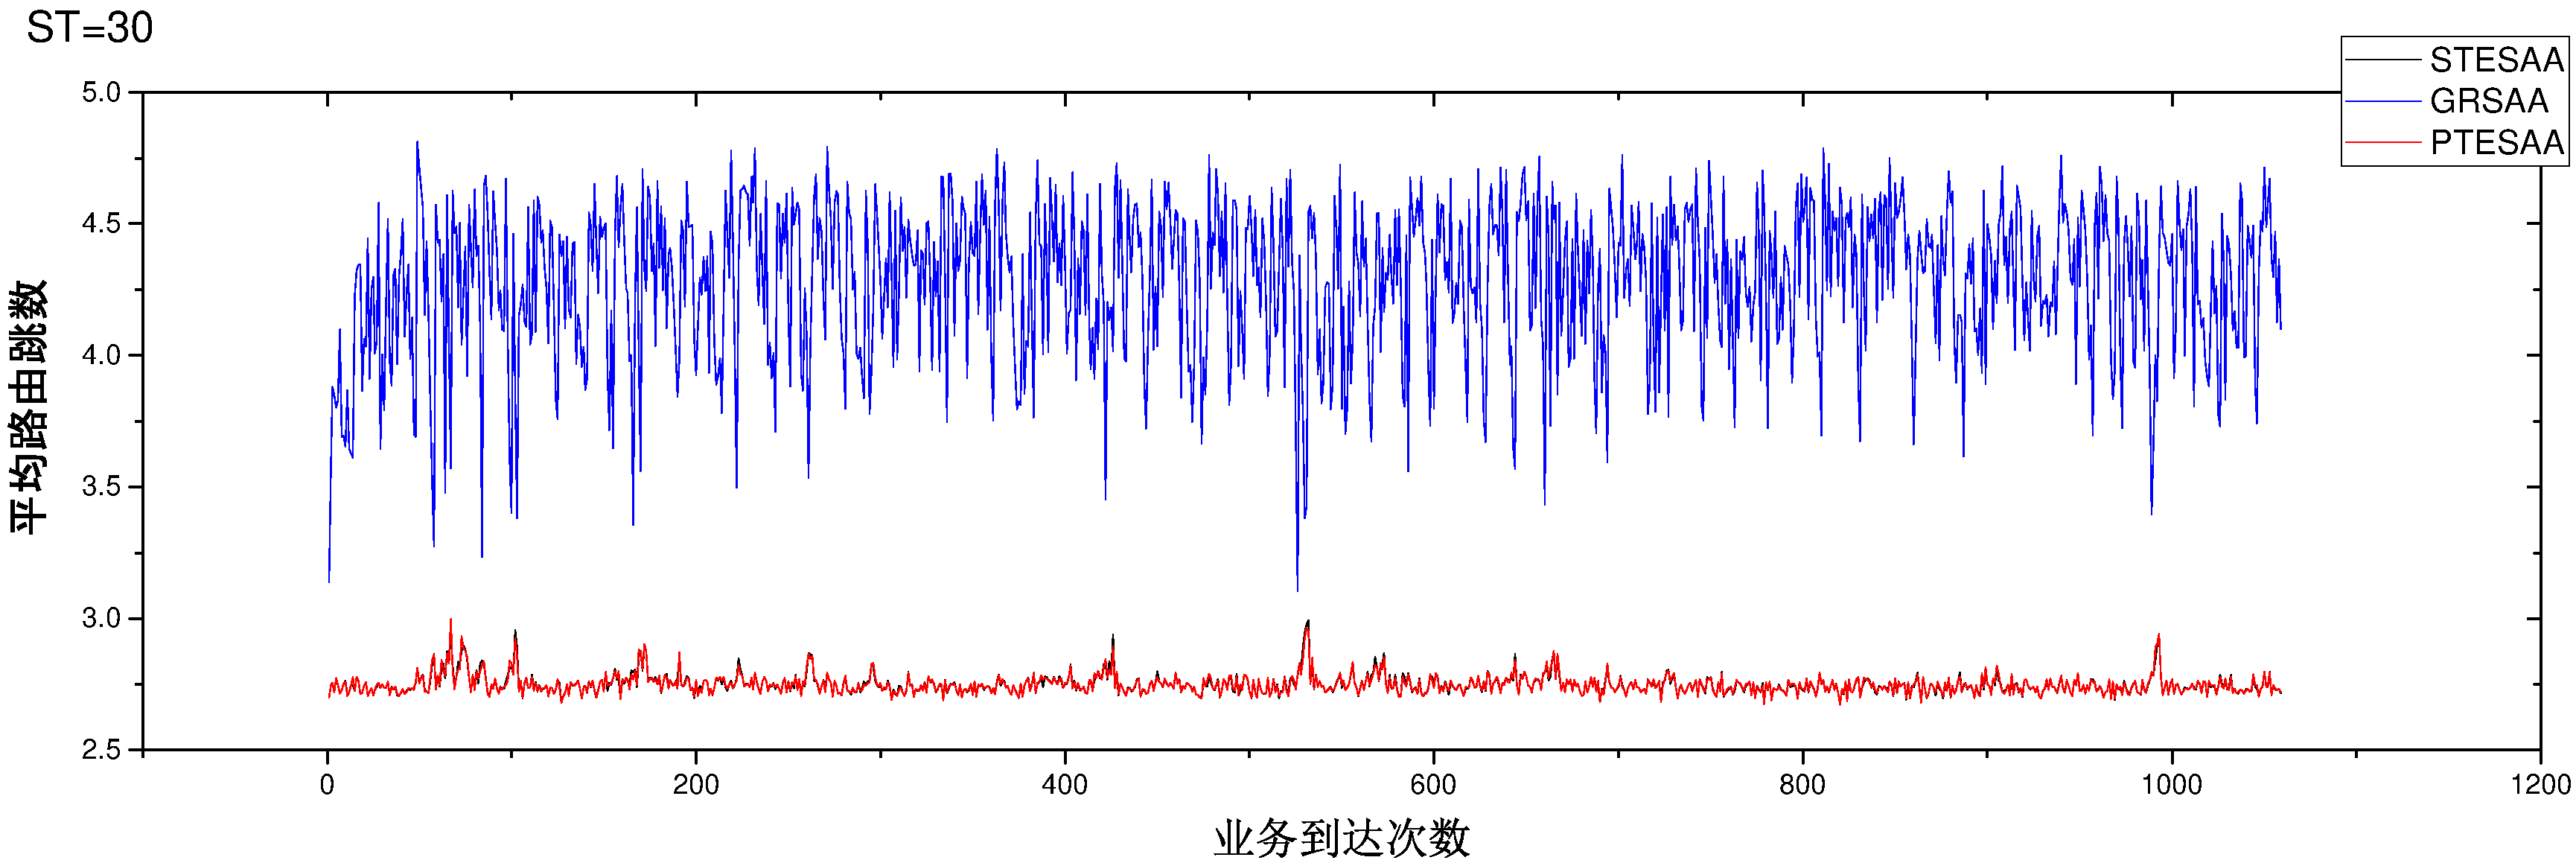
\includegraphics[width=1 \textwidth]{figures/B30H.pdf}}
\end{center}
\caption{{\footnotesize{无权图路径跳数对比(ST=30)}}}
\label{B20H}
\end{figure*}
\begin{figure*}
\vspace{-0.5cm}
\setlength{\abovecaptionskip}{-0.5cm}
%\setlength{\belowcaptionskip}{-1cm}
\begin{center}
{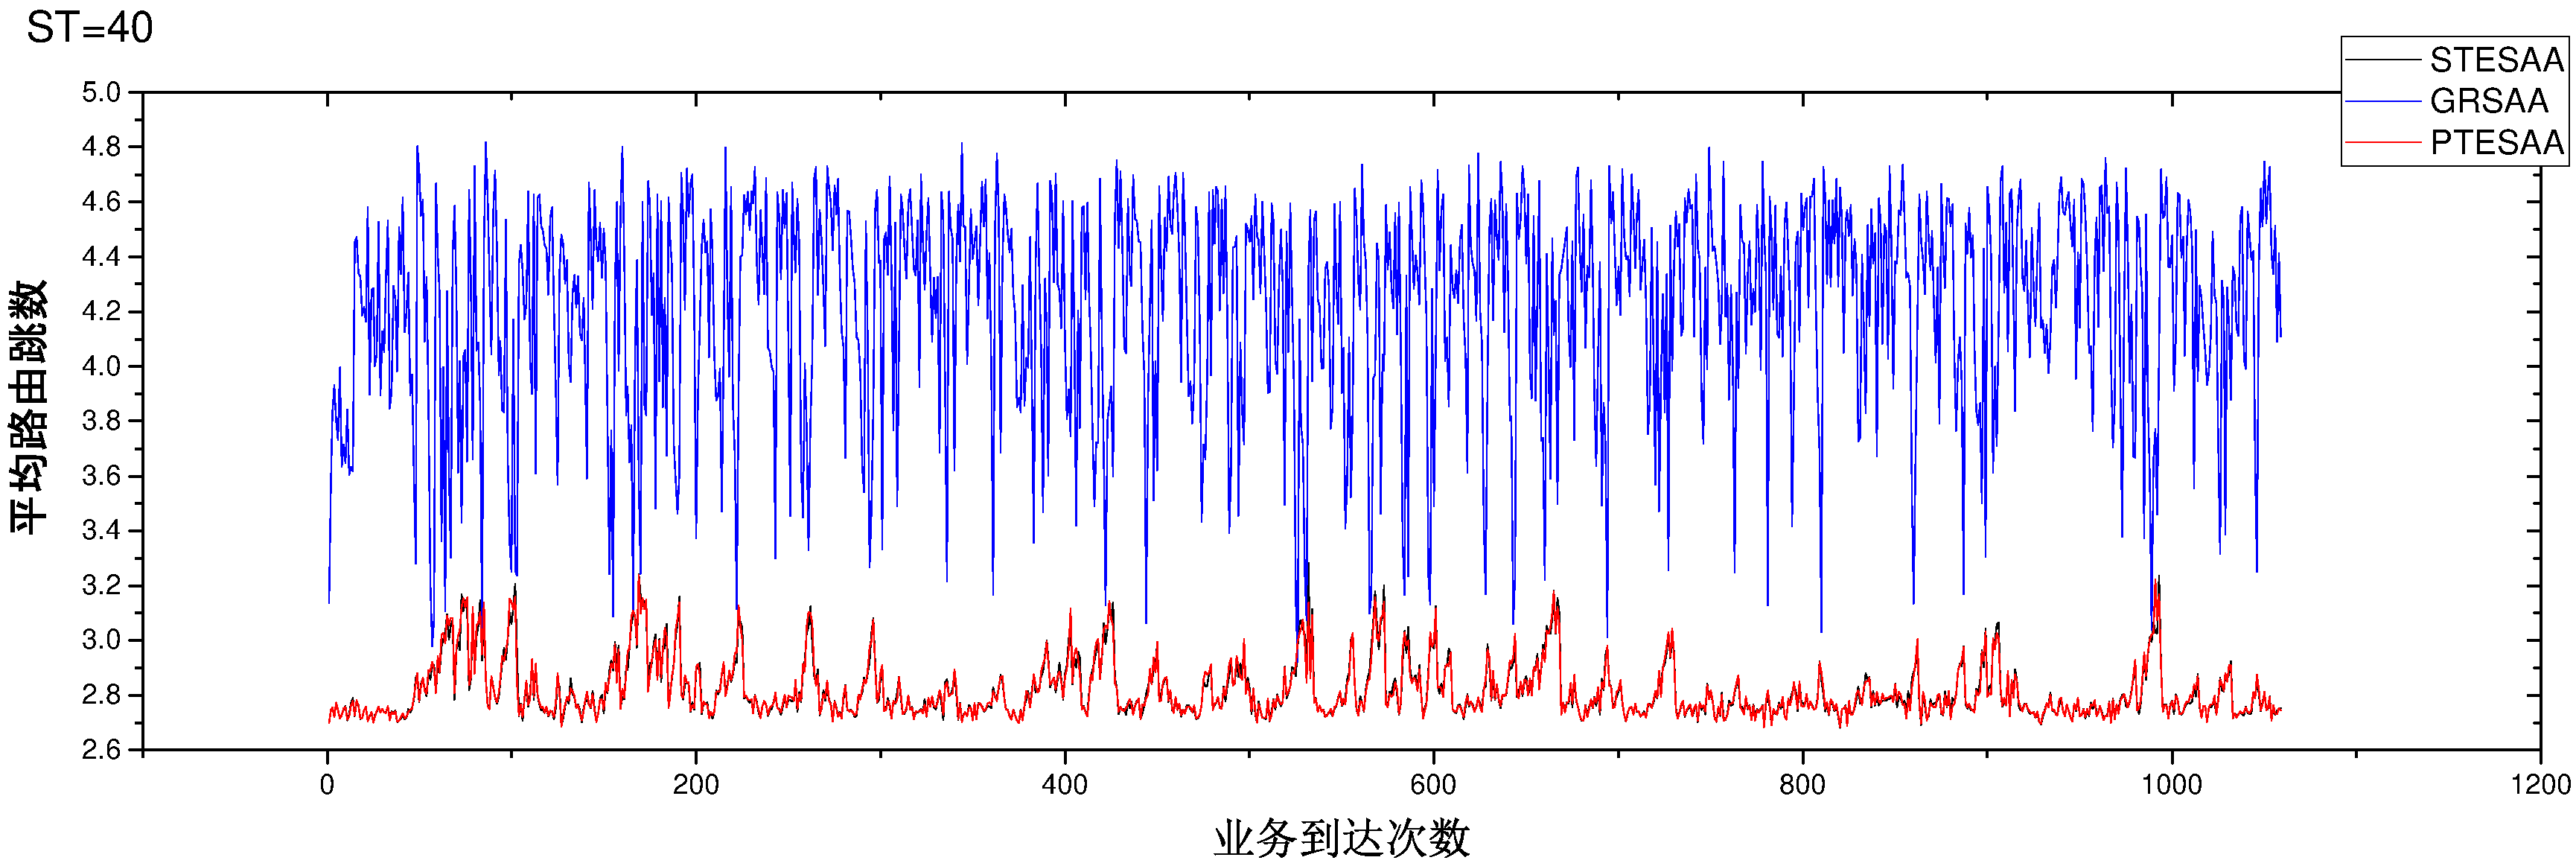
\includegraphics[width=1 \textwidth]{figures/B40H.pdf}}
\end{center}
\caption{{\footnotesize{无权图路径跳数对比(ST=40)}}}
\label{B40H}
\end{figure*}
\subsubsection{时间分析}

图 \ref{B5T}到图 \ref{B40T}展示了各个算法在不同平均服务时间$ST$下的计算时间,当$ST=5$时,我们可以看到通过GPU加速的PTESAA的计算时间是STESAA计算时间的1/4,而实际上,步骤一的GPU加速比可达7-8倍,但是由于步骤二的快速路由选择算法所占用的时间也不可忽略,而我们没有对这部分算法进行GPU加速,这使得总体的加速比下降为4-5倍。

图\ref{B5T}到图\ref{B40T}显示GRSAA的计算时间略高于PTESAA的计算时间,可见PTESAA不仅可以优化路由跳数,而且在时间上也比GRSAA更有优势。

观察图\ref{B5T}到图\ref{B40T},我们发现随着$ST$的变化,PTESAA对STESAA的加速比略有下降,这是因为随着网络压力的增加,可用链路变少,使得STESAA中步骤一的计算量下降,PTESAA的加速优势变小。
\begin{figure*}
\vspace{-0.5cm}
\setlength{\abovecaptionskip}{-0.5cm}
%\setlength{\belowcaptionskip}{-0.1cm}
\begin{center}
{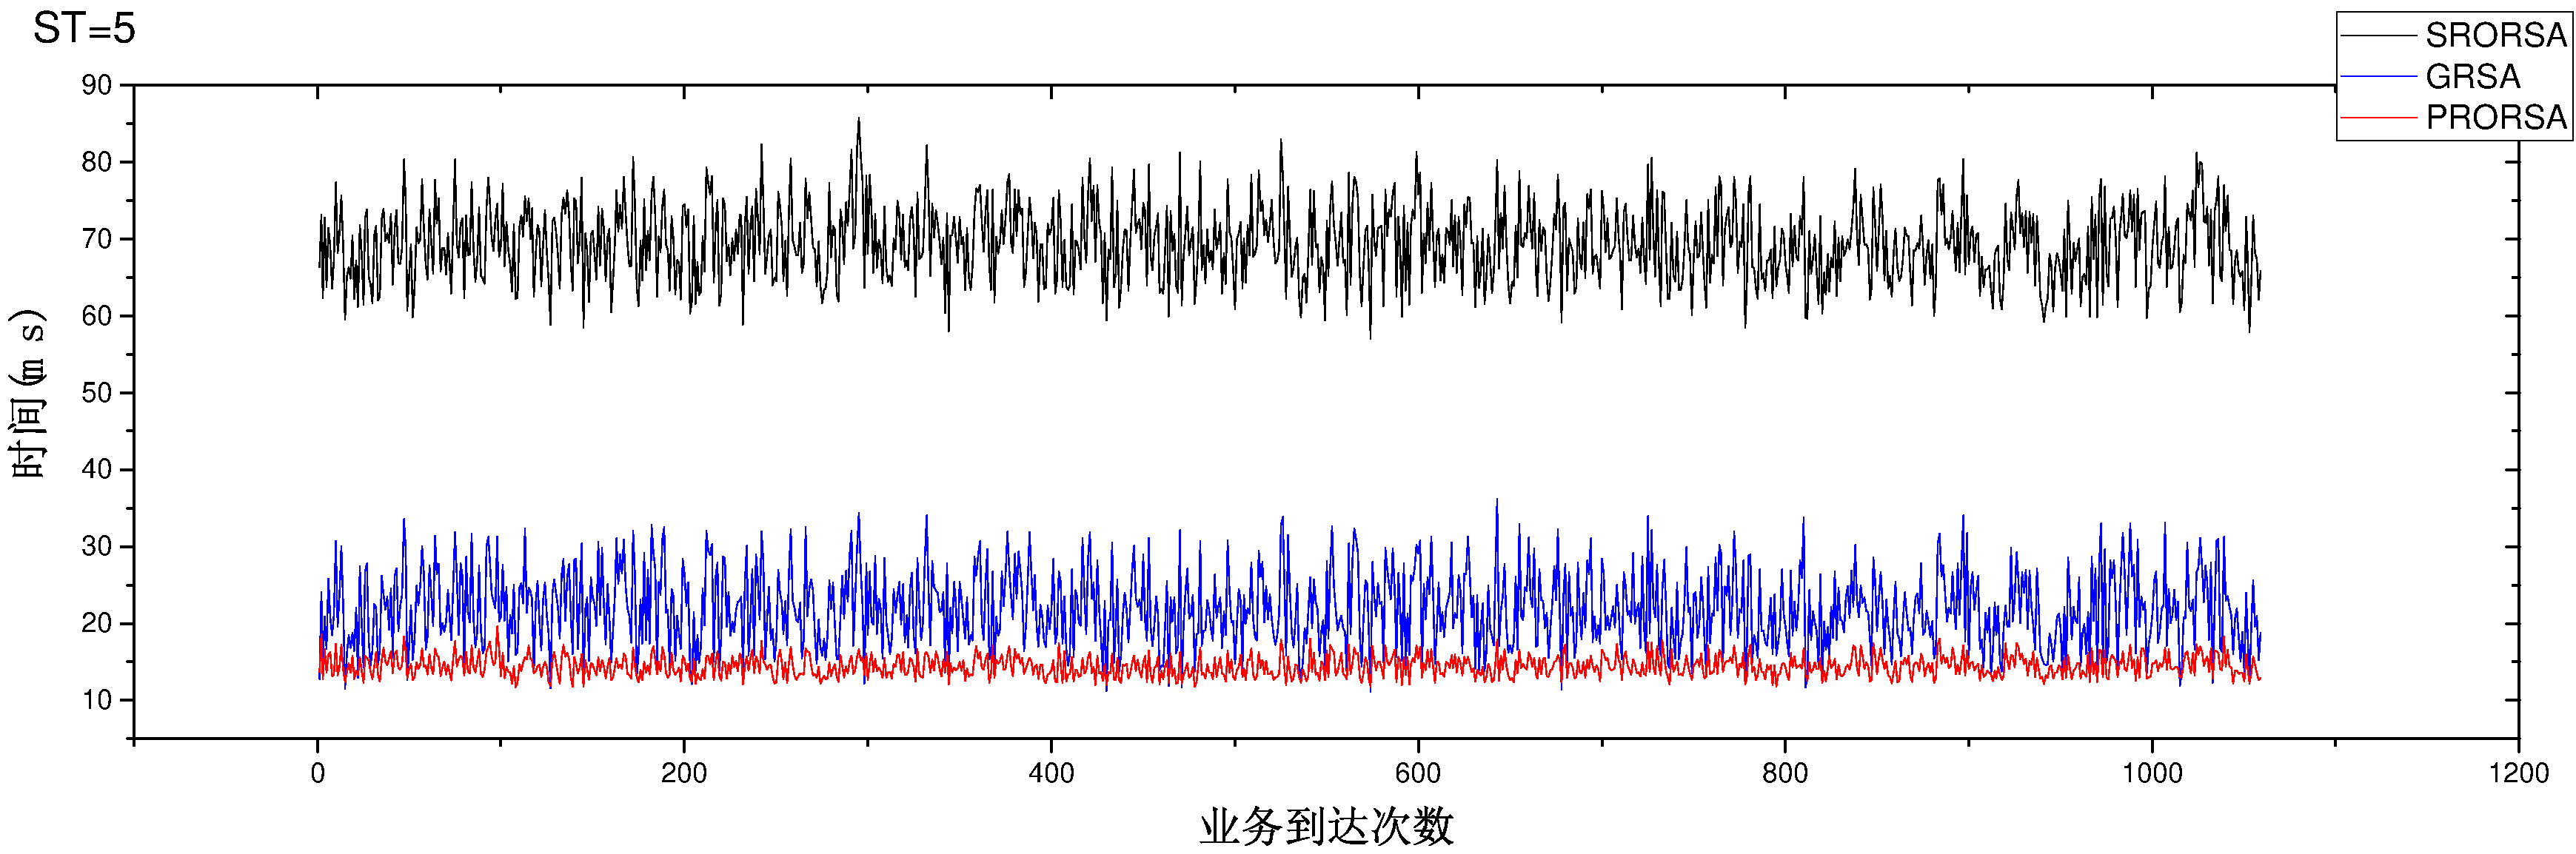
\includegraphics[width=1 \textwidth]{figures/B5T.pdf}}
\end{center}
\caption{{\footnotesize{无权图时间对比(ST=5)}}}
\label{B5T}
\end{figure*}
\begin{figure*}
\vspace{-0.5cm}
\setlength{\abovecaptionskip}{-0.5cm}
%\setlength{\belowcaptionskip}{-0.5cm}
\begin{center}
{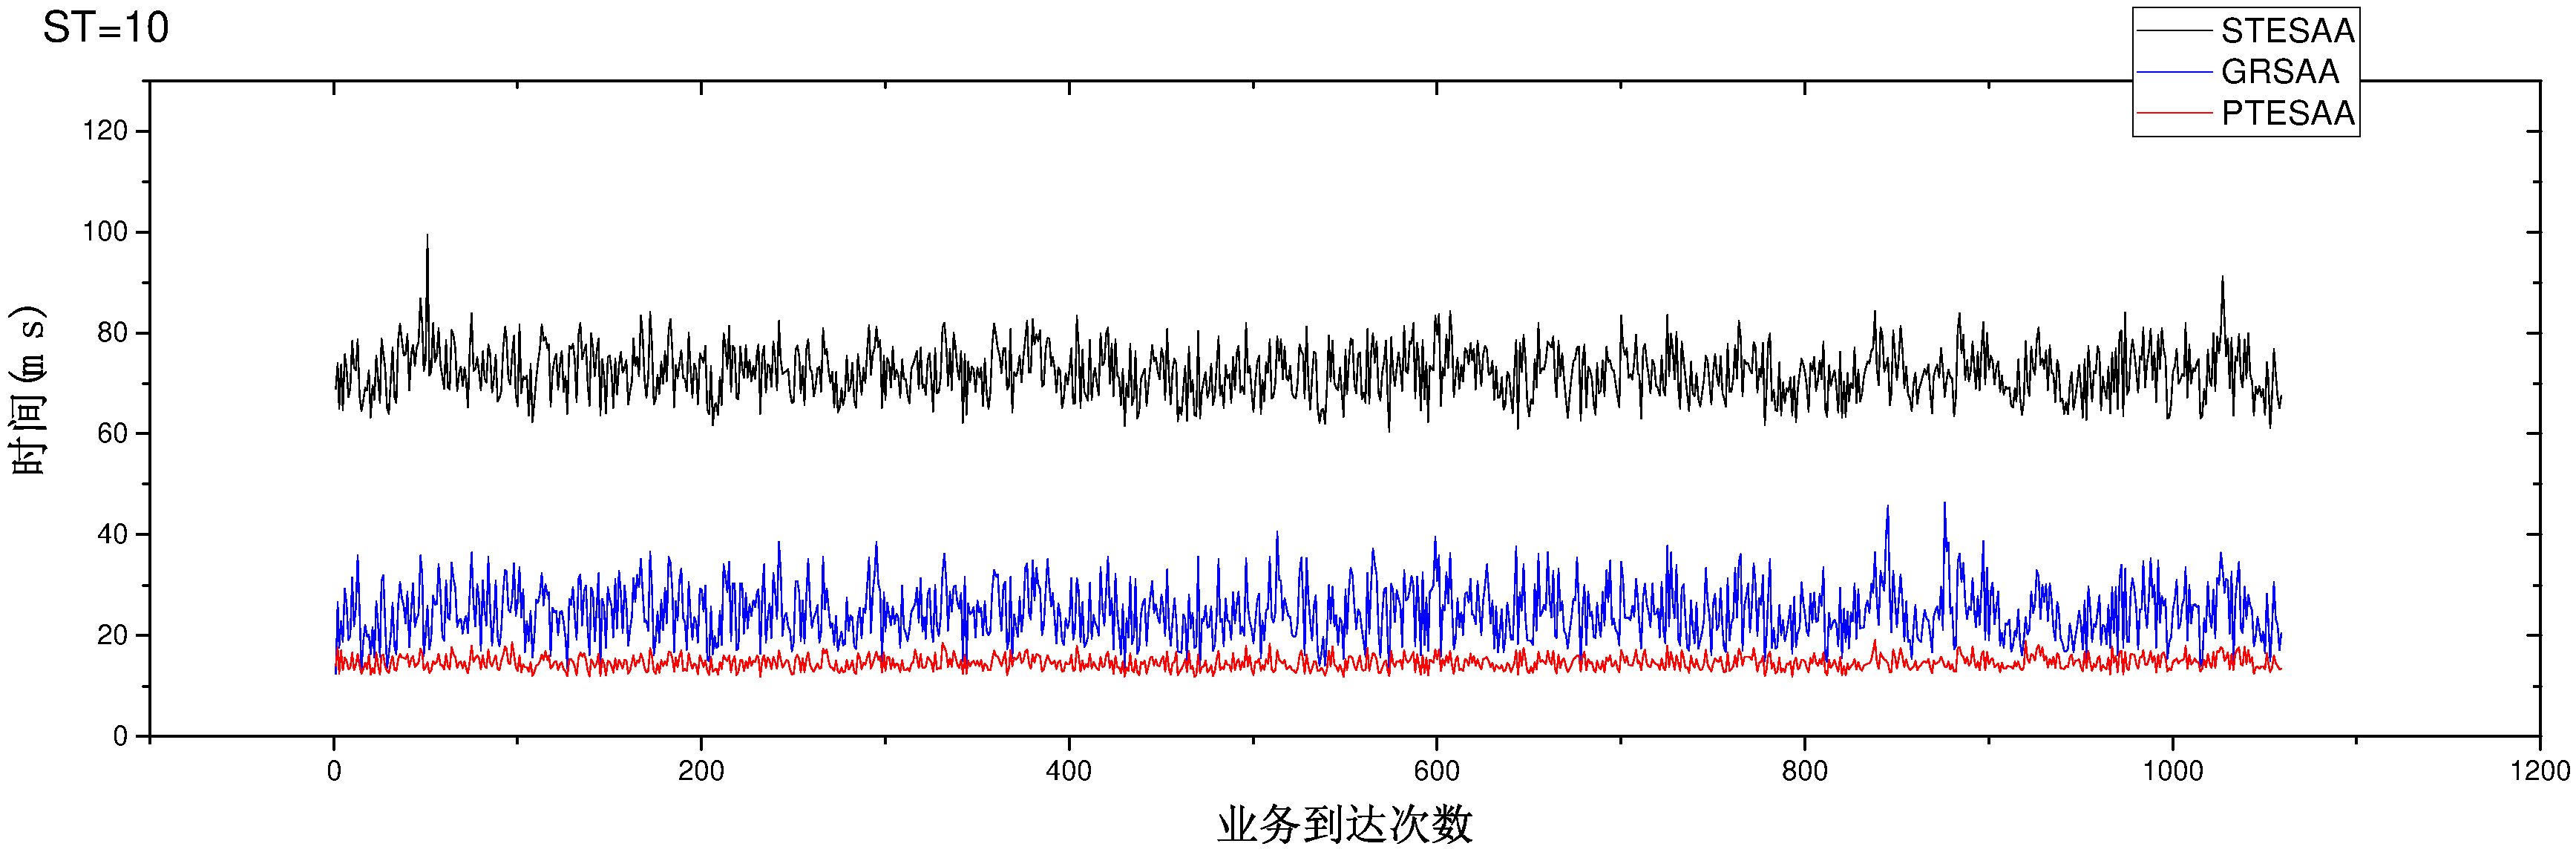
\includegraphics[width=1 \textwidth]{figures/B10T.pdf}}
\end{center}
\caption{{\footnotesize{无权图时间对比(ST=10)}}}
\label{B10T}
\end{figure*}
\begin{figure*}
\vspace{-0.5cm}
\setlength{\abovecaptionskip}{-0.5cm}
\begin{center}
{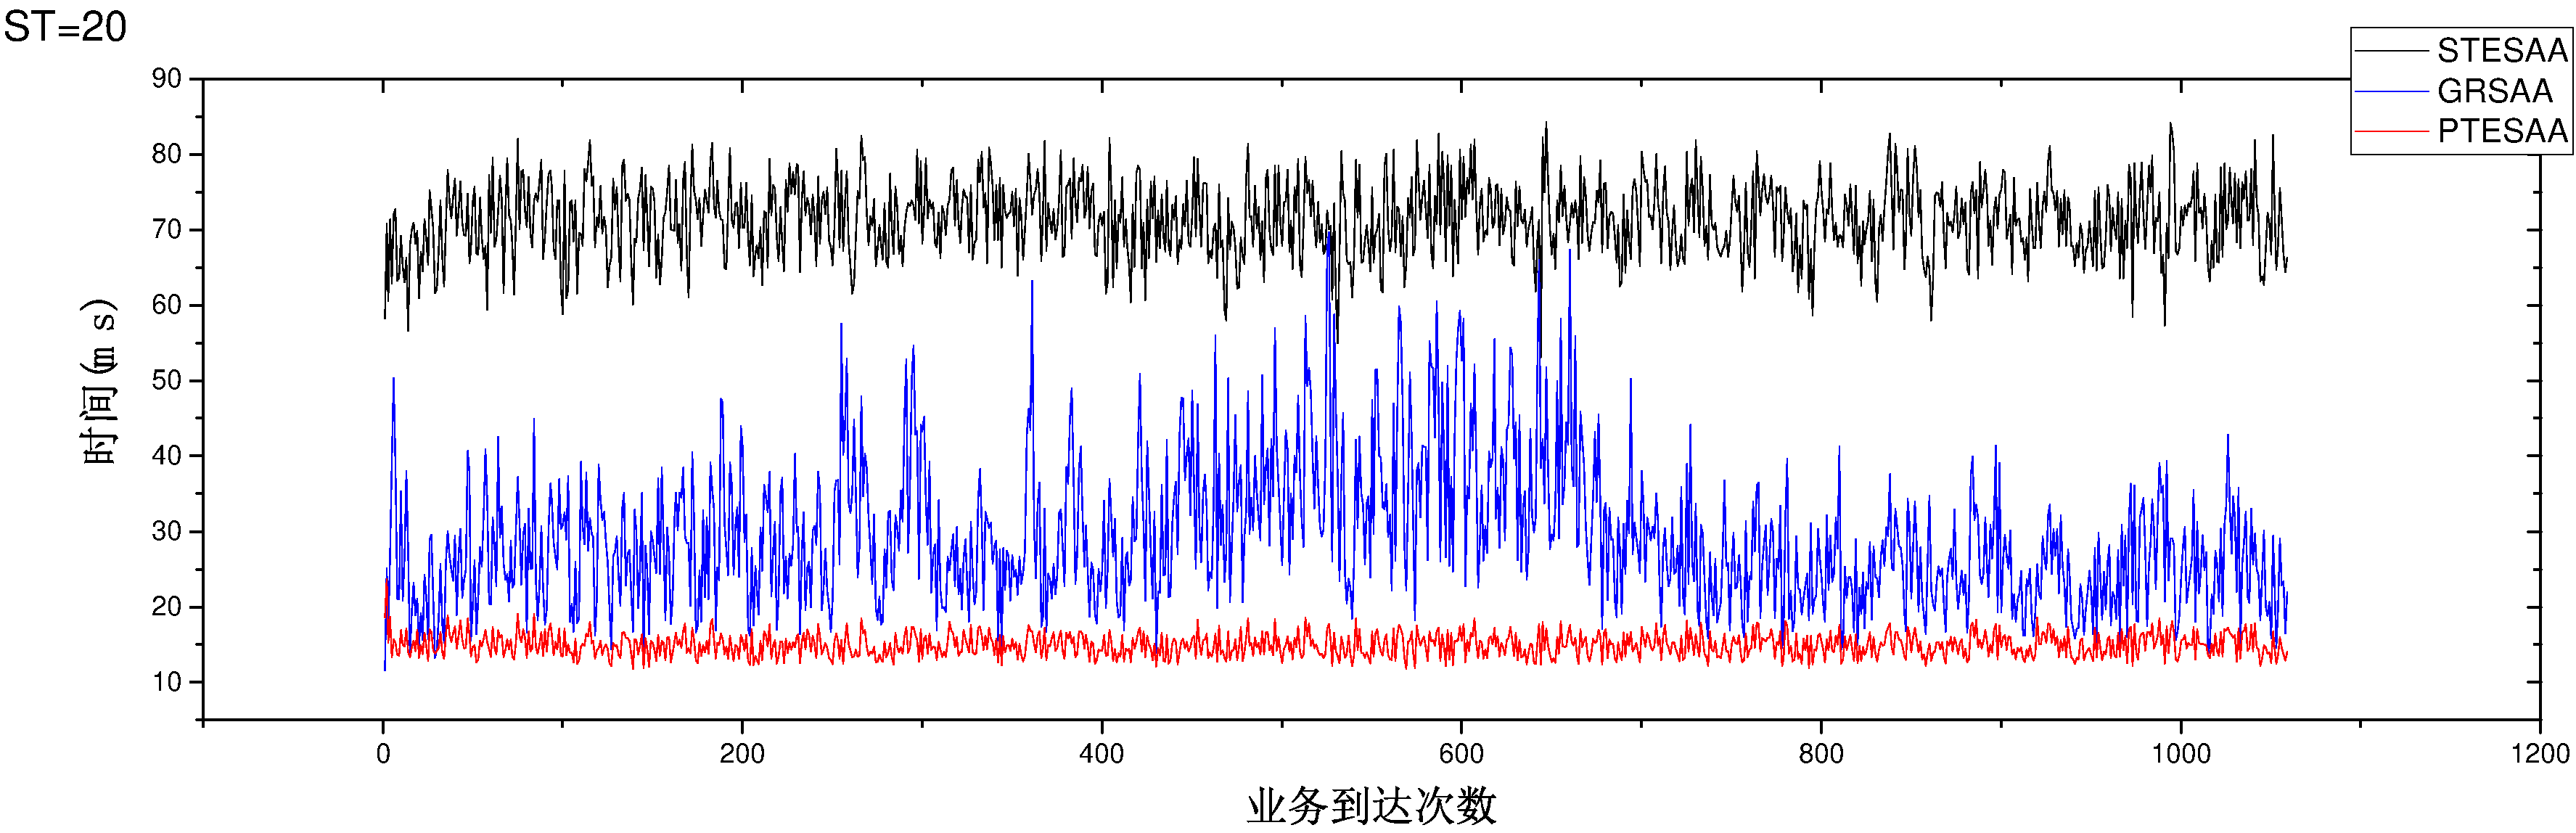
\includegraphics[width=1 \textwidth]{figures/B20T.pdf}}
\end{center}
\caption{{\footnotesize{无权图时间对比(ST=20)}}}
\label{B20T}
\end{figure*}
\begin{figure*}
\vspace{-0.5cm}
\setlength{\abovecaptionskip}{-0.5cm}
\begin{center}
{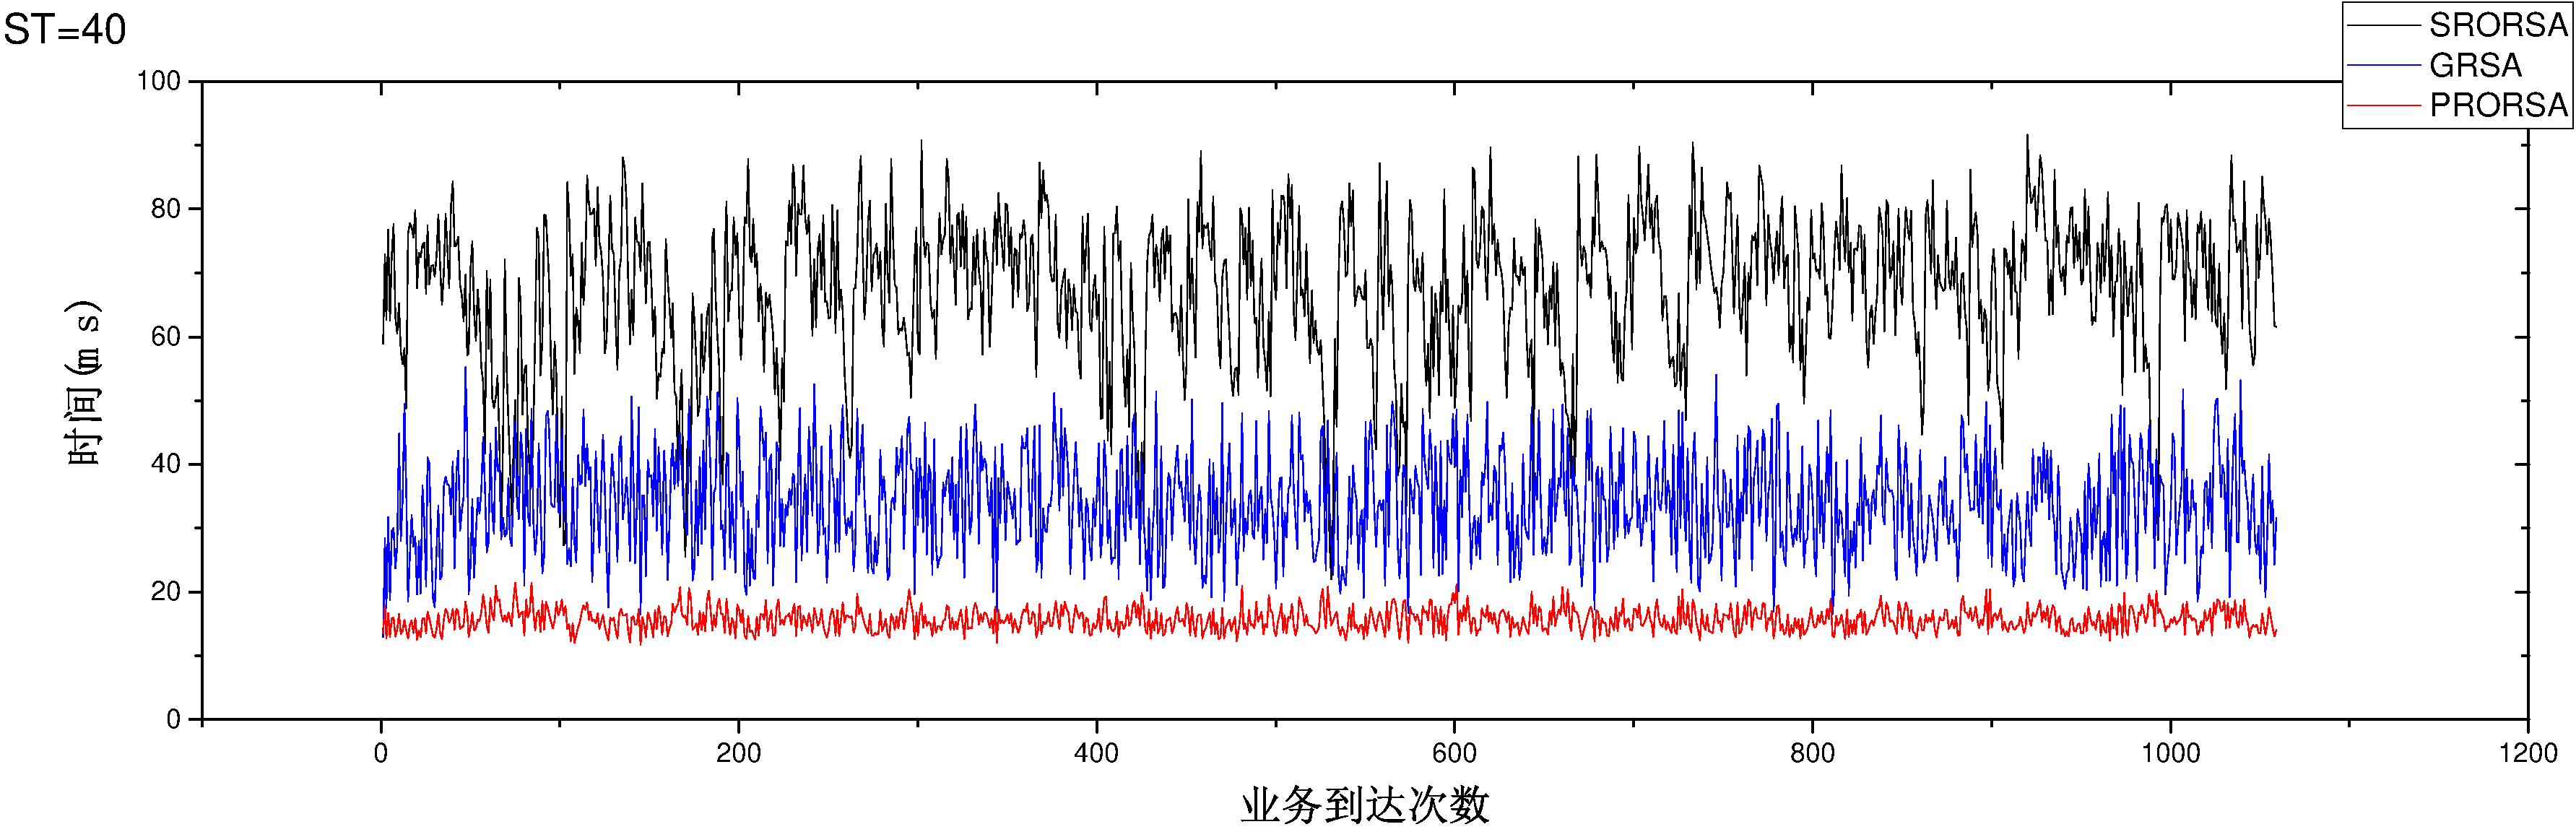
\includegraphics[width=1 \textwidth]{figures/B40T.pdf}}
\end{center}
\caption{{\footnotesize{无权图时间对比(ST=40)}}}
\label{B40T}
\end{figure*}
\subsubsection{阻塞率分析}

图 \ref{B10Z}到图 \ref{B40Z}展示了随着$ST$的增加,PTESAA/STESAA和GRSAA算法的阻塞率变化情况。其中PTESAA,STESAA由于是同一种算法,所以其阻塞率几乎一样。当$ST=10$时,我们发现PTESAA/STESAA的阻塞次数明显小于GRSAA。 当$ST=20$时,PTESAA/STESAA的阻塞次数和阻塞幅度均小于GRSAA,在GRSAA中出现了一次相对较大的阻塞,但是PTESAA/STESAA中没有出现这种不平稳的阻塞率突变。当$ST=30$时,我们发现PTESAA/STESAA的阻塞次数和阻塞幅度比GRSAA小很多,GRSAA的平均阻塞率是PTESAA/STESAA的6倍左右。当$ST=40$时,PTESAA,STESAA和GRSAA的阻塞率都增加很多,但是PTESAA/STESAA的阻塞情况还是大大优于GRSAA,可见在网络拥塞的情况下,PTESAA/STESAA依然能够有效地减小阻塞率。
\begin{figure*}
\setlength{\abovecaptionskip}{-0.5cm}
\begin{center}
{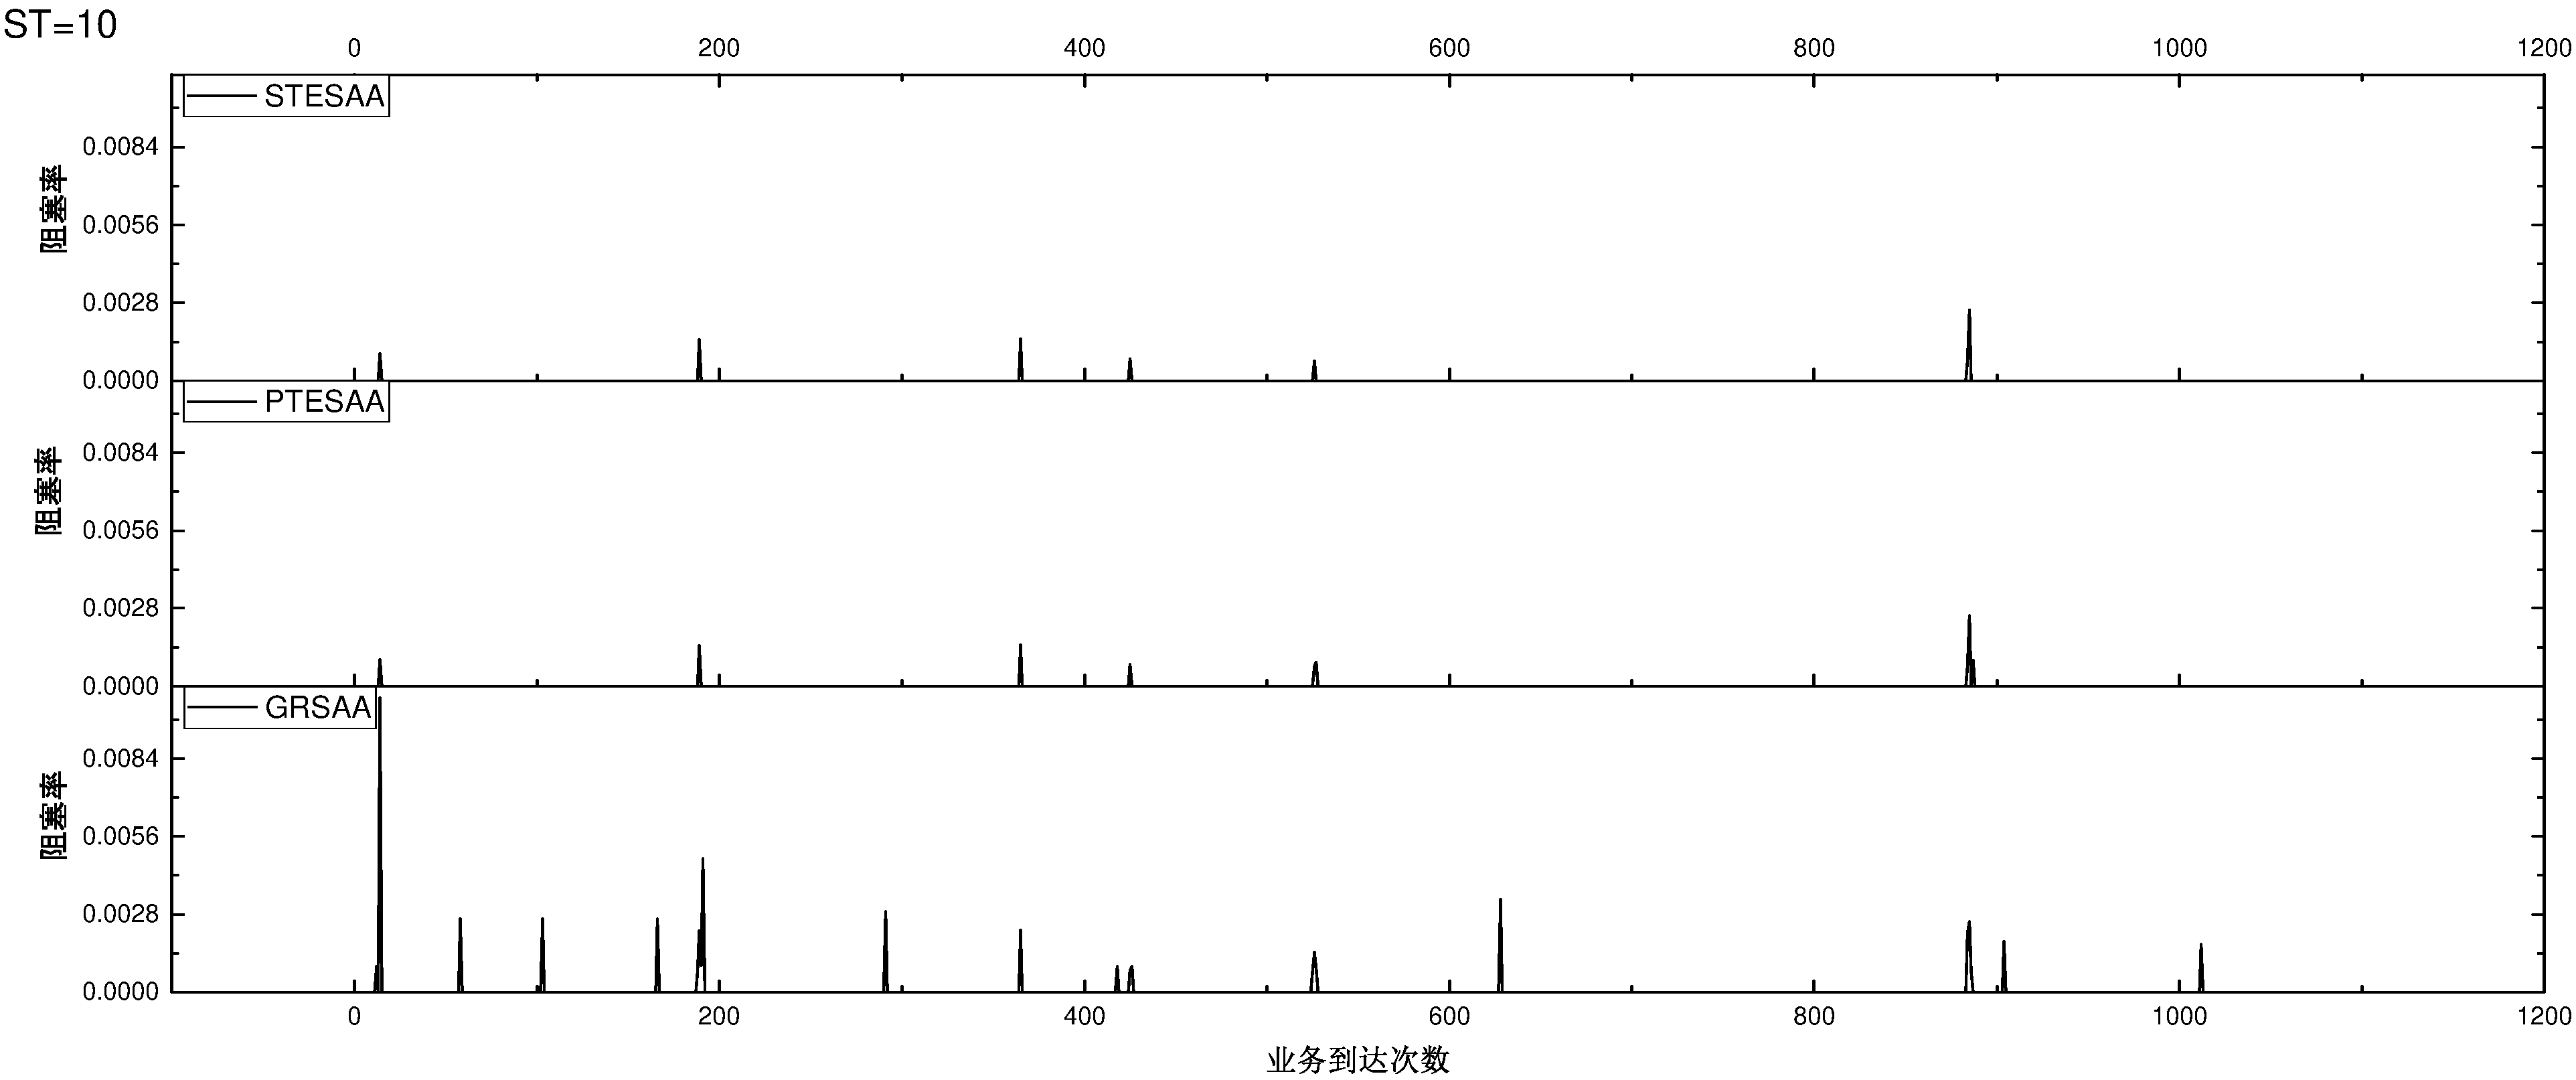
\includegraphics[width=1 \textwidth]{figures/B10Z.pdf}}
\end{center}
\caption{{\footnotesize{无权图阻塞率对比(ST=10)}}}
\label{B10Z}
\end{figure*}
\begin{figure*}
\setlength{\abovecaptionskip}{-0.5cm}
\begin{center}
{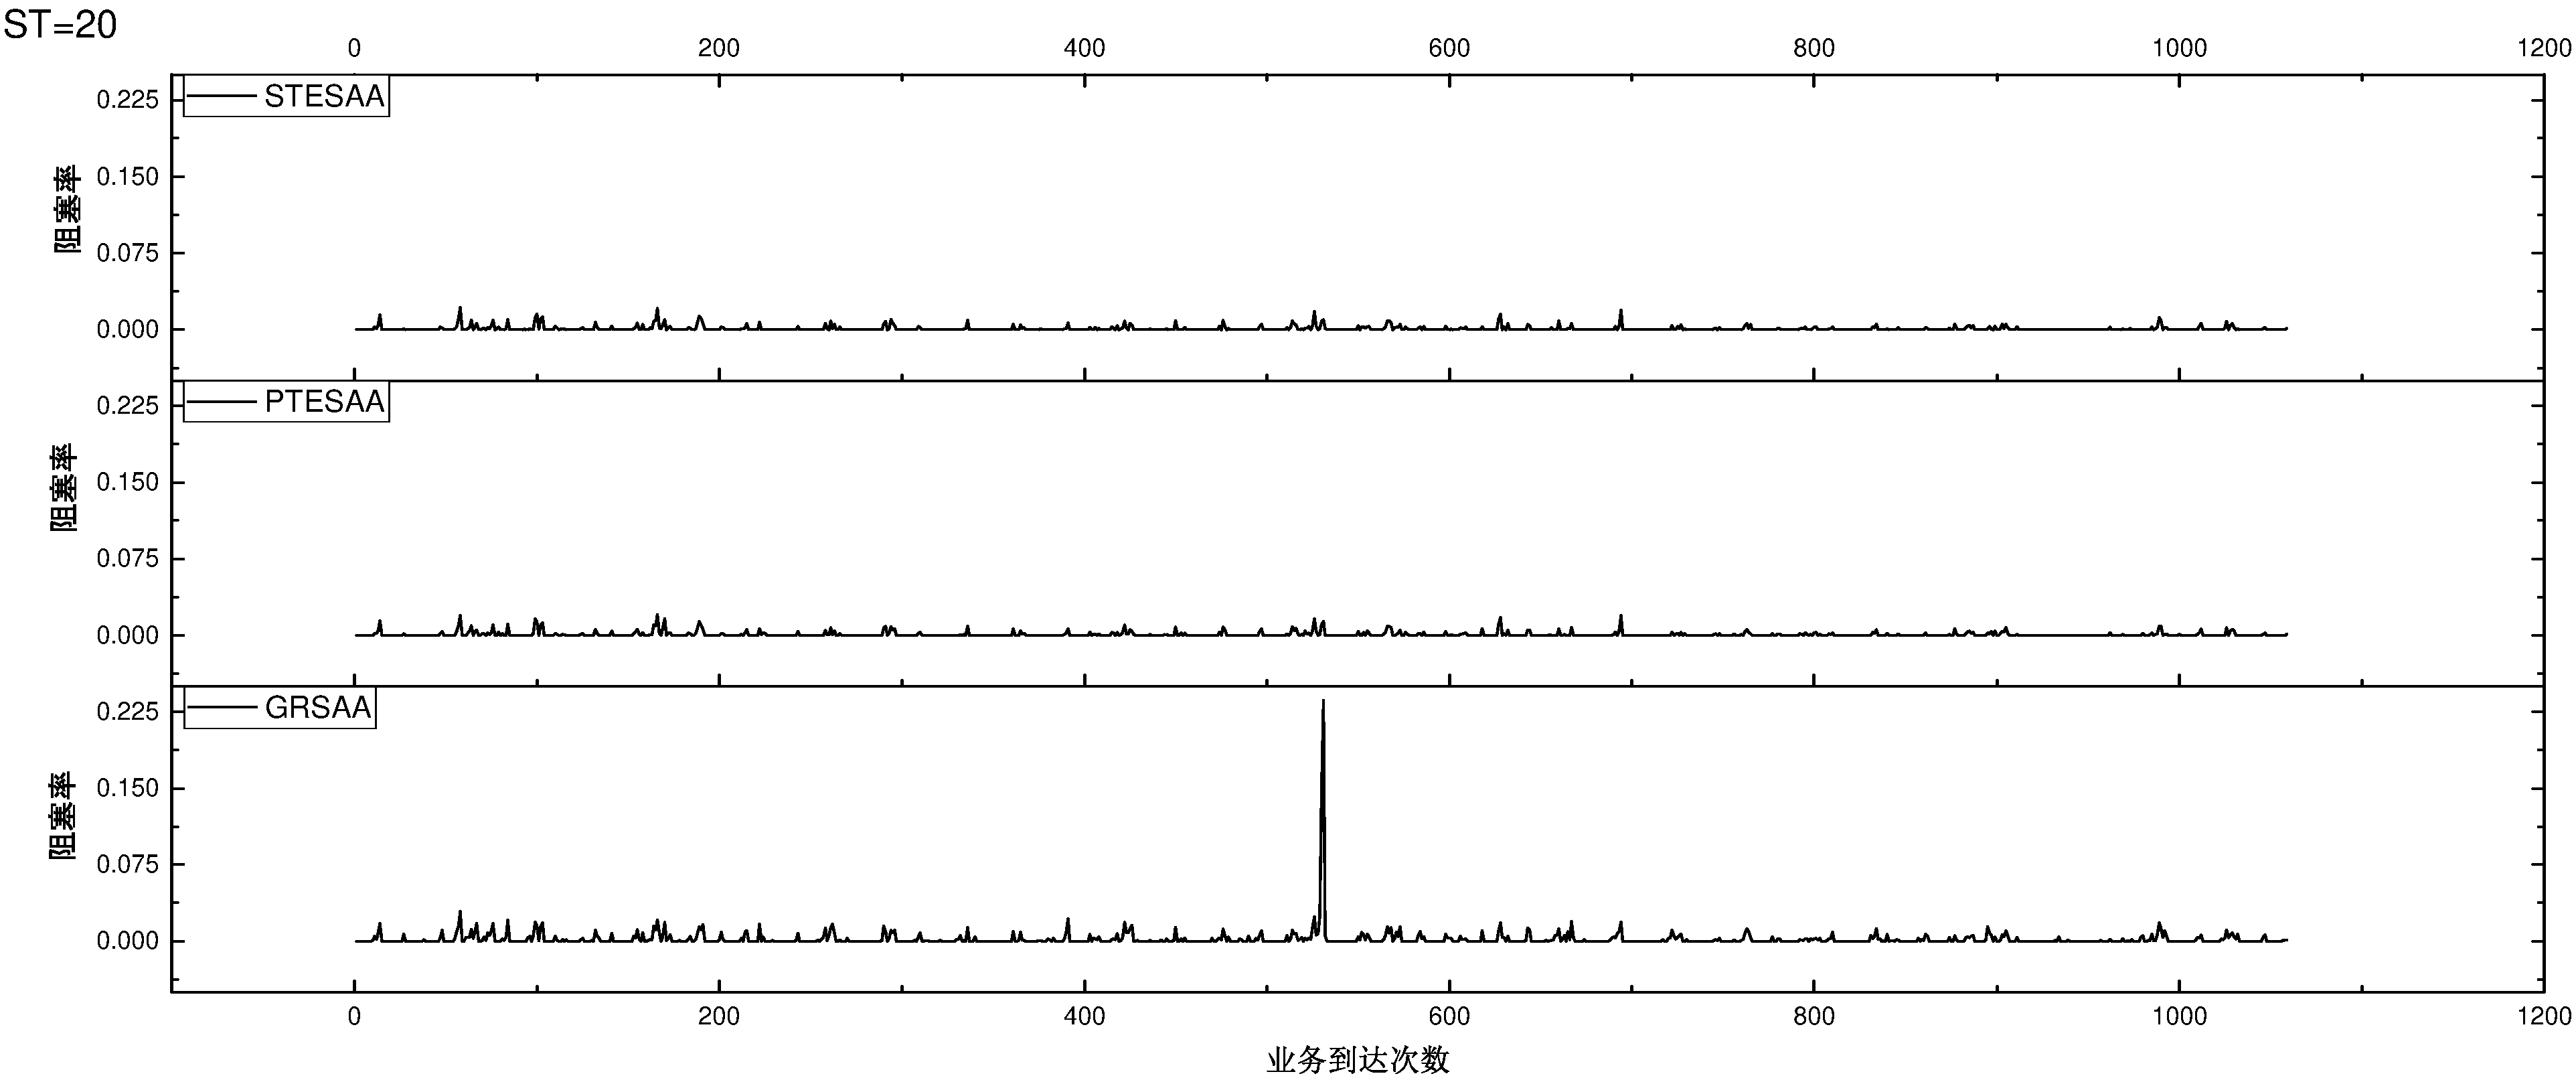
\includegraphics[width=1 \textwidth]{figures/B20Z.pdf}}
\end{center}
\caption{{\footnotesize{无权图阻塞率对比(ST=20)}}}
\label{B20Z}
\end{figure*}
\begin{figure*}
\setlength{\abovecaptionskip}{-0.5cm}
\begin{center}
{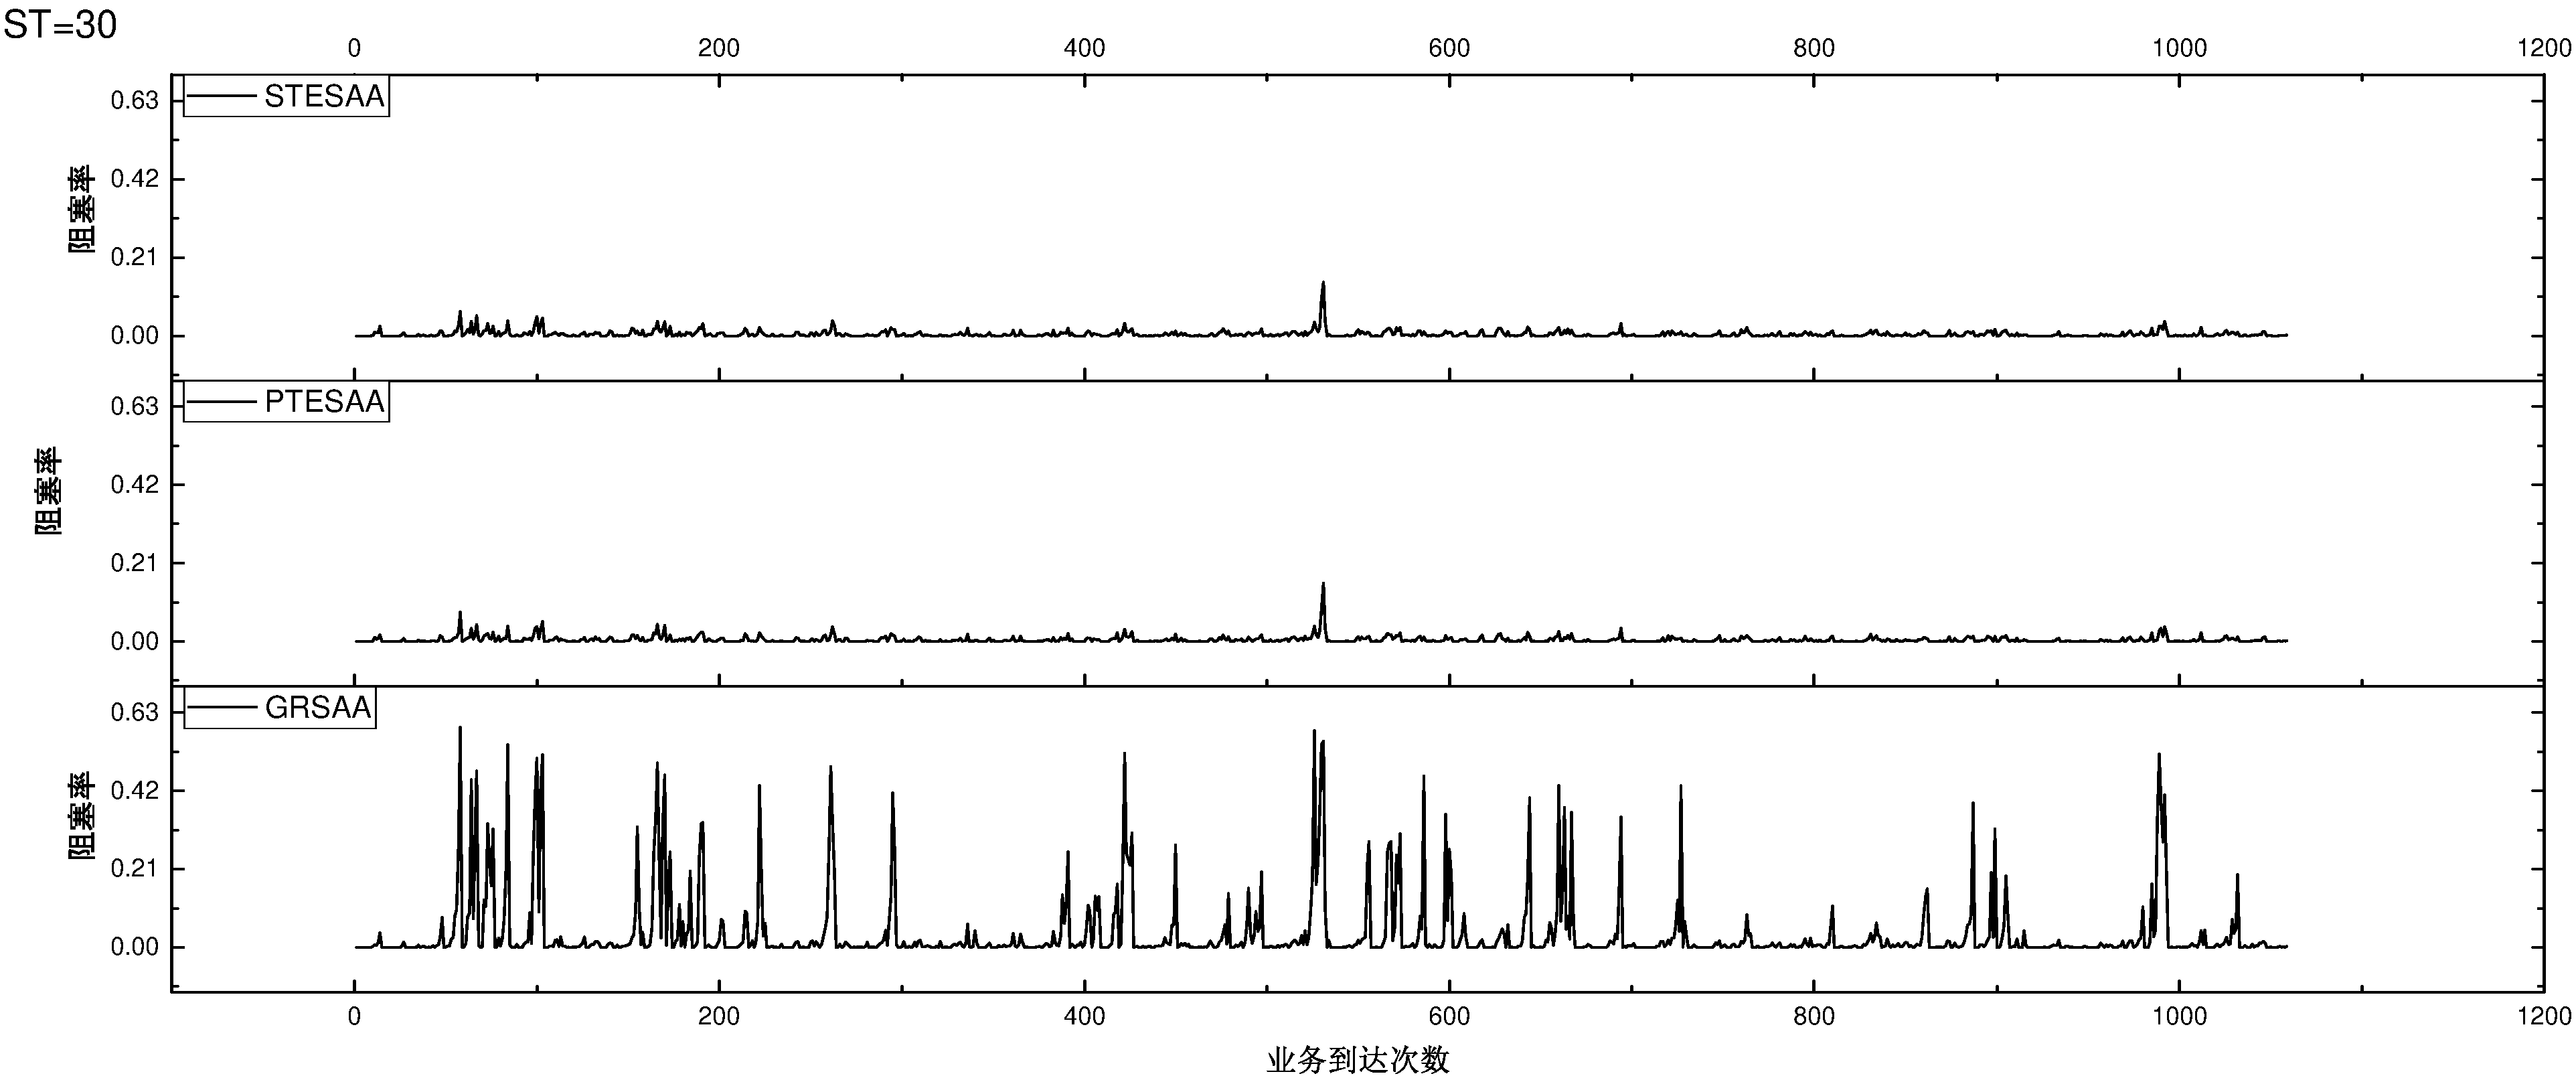
\includegraphics[width=1 \textwidth]{figures/B30Z.pdf}}
\end{center}
\caption{{\footnotesize{无权图阻塞率对比(ST=30)}}}
\label{B40Z}
\end{figure*}
\begin{figure*}
\setlength{\abovecaptionskip}{-0.5cm}
\begin{center}
{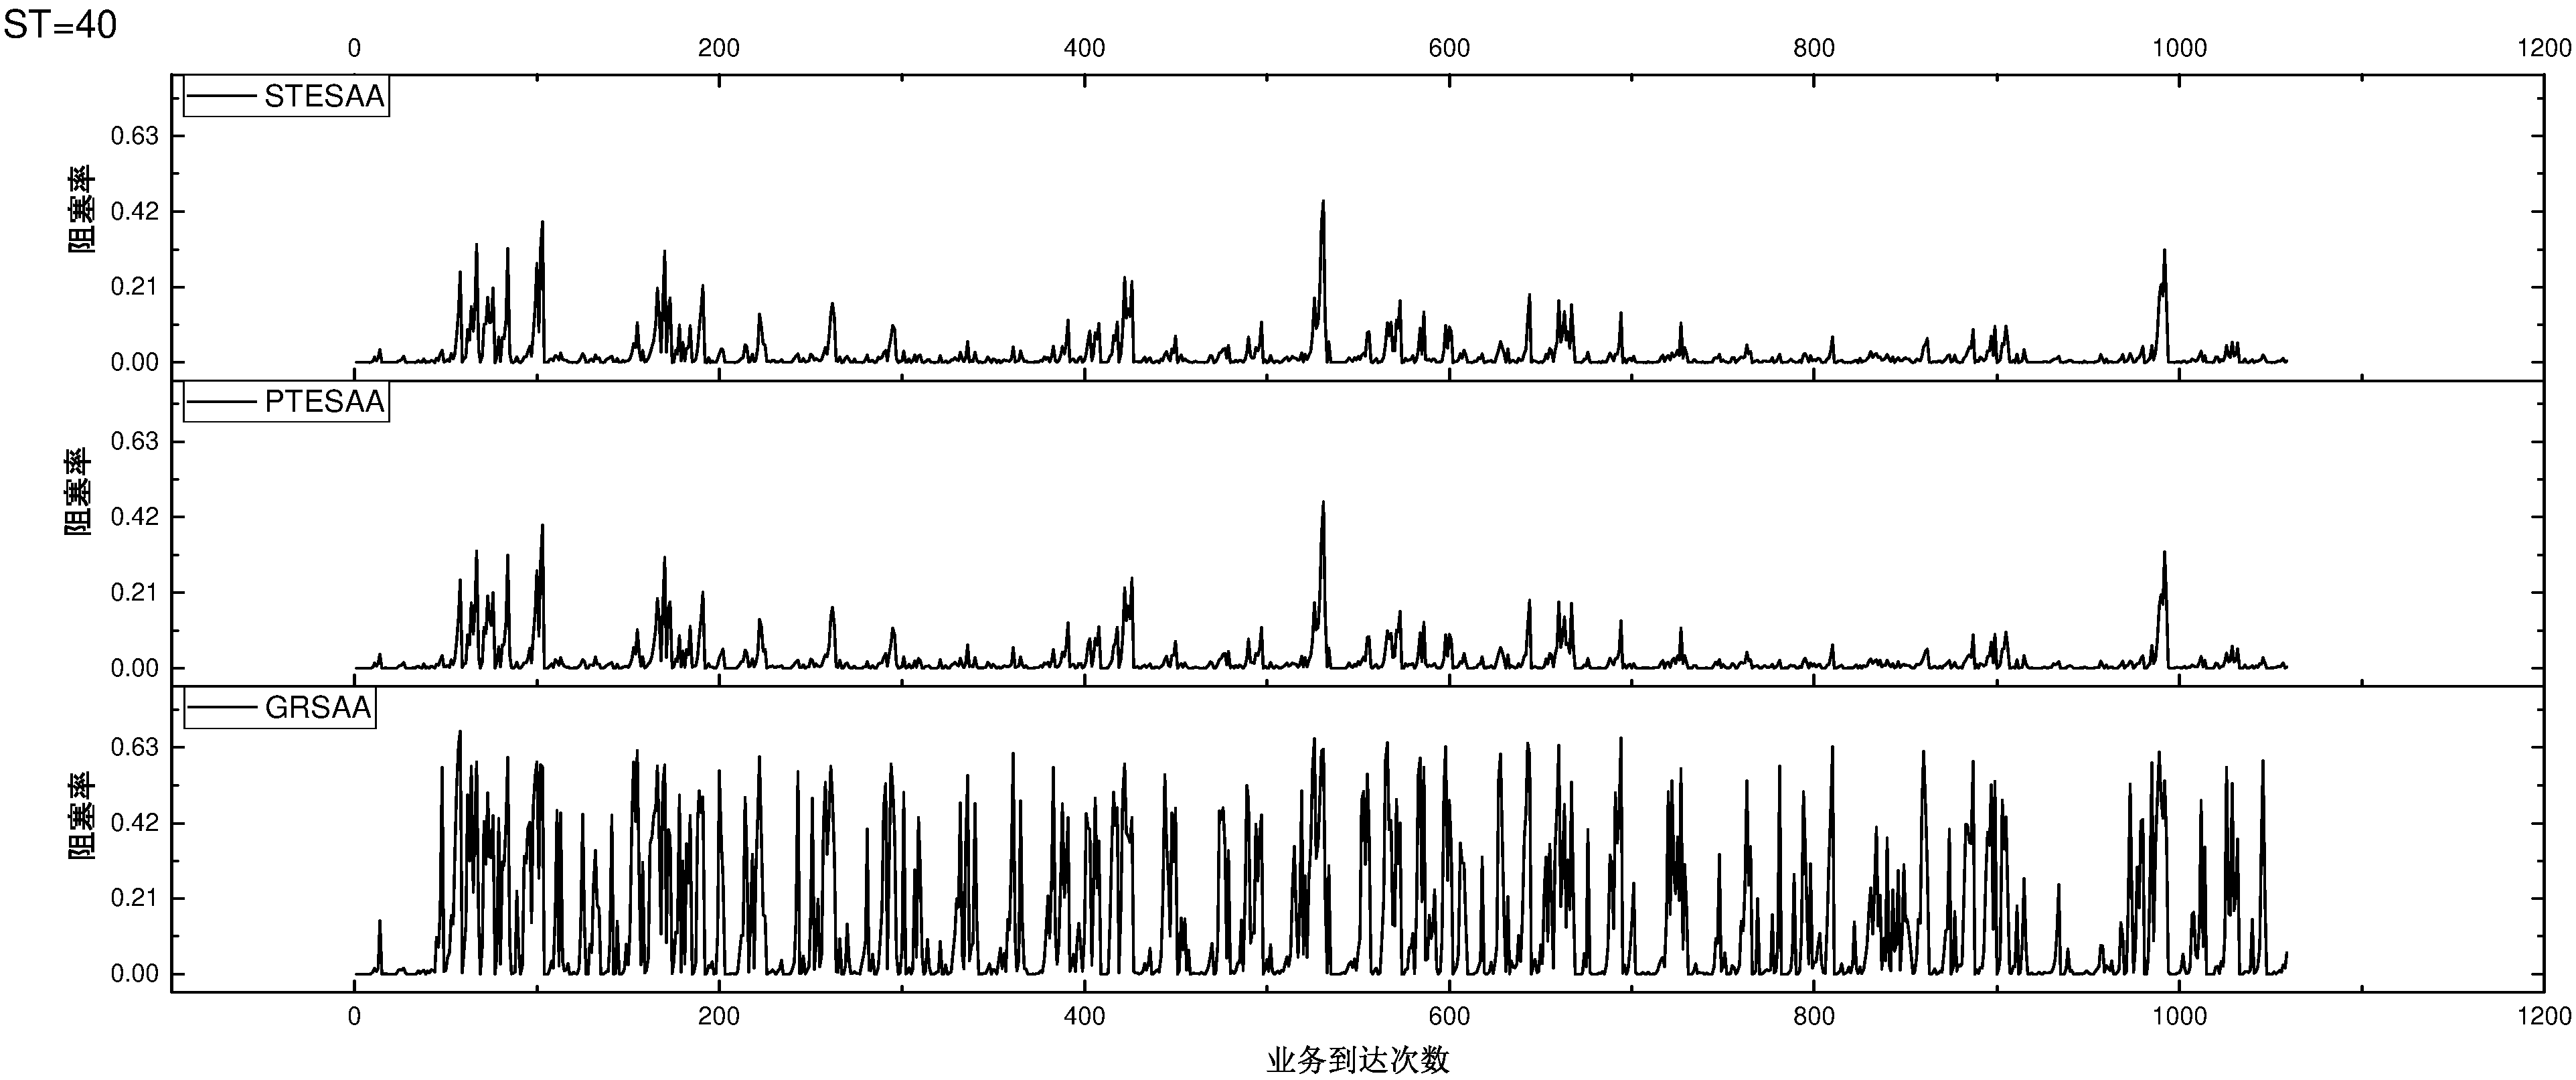
\includegraphics[width=1 \textwidth]{figures/B40Z.pdf}}
\end{center}
\caption{{\footnotesize{无权图阻塞率对比(ST=40)}}}
\label{B40Z}
\end{figure*}
\subsection{带权图下的仿真结果}
\subsubsection{路由代价优化结果分析}
\begin{figure*}
\vspace{-0.5cm}
\setlength{\abovecaptionskip}{-0.5cm}
\begin{center}
{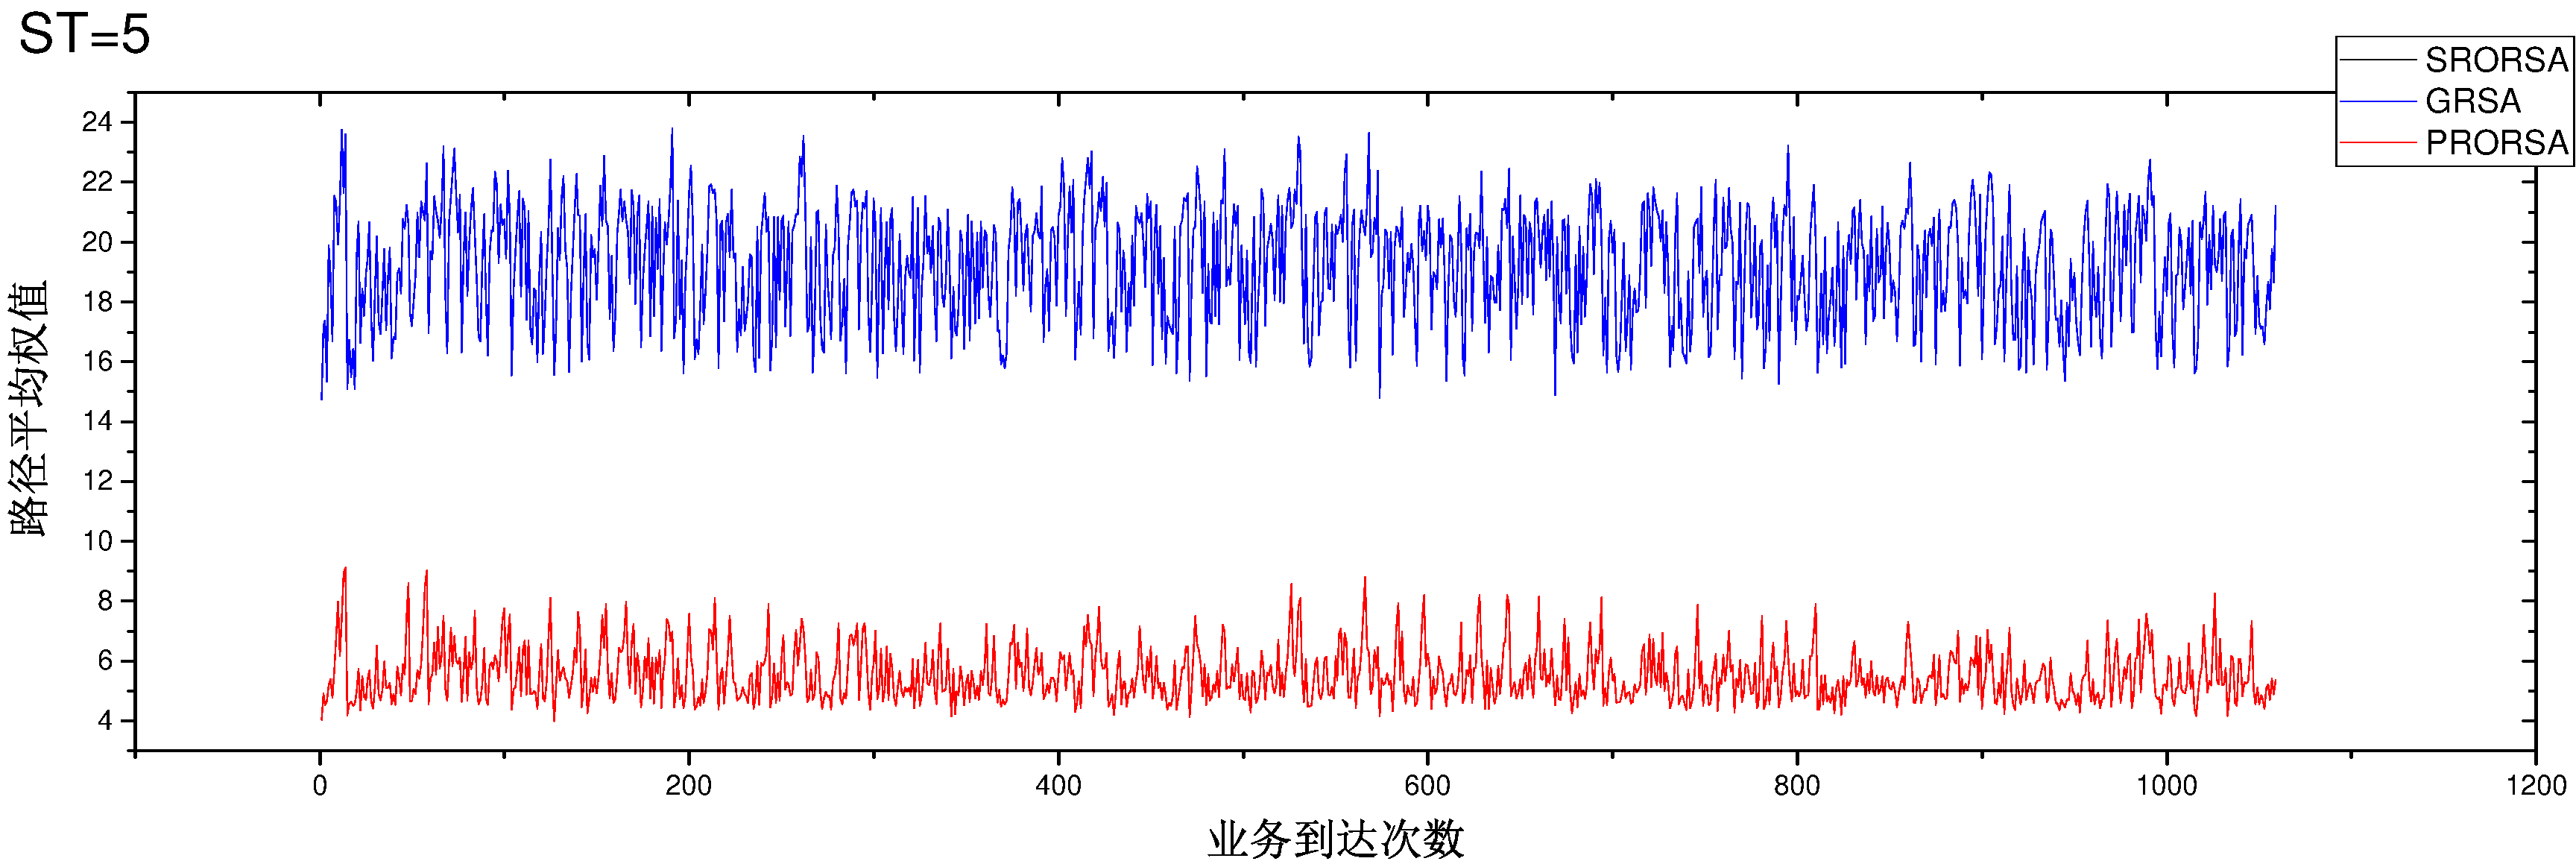
\includegraphics[width=1 \textwidth]{figures/H5C.pdf}}
\end{center}
\caption{{\footnotesize{带权图路由代价对比(ST=5)}}}
\label{H5C}
\end{figure*}
\begin{figure*}
\vspace{-0.5cm}
\setlength{\abovecaptionskip}{-0.5cm}
\begin{center}
{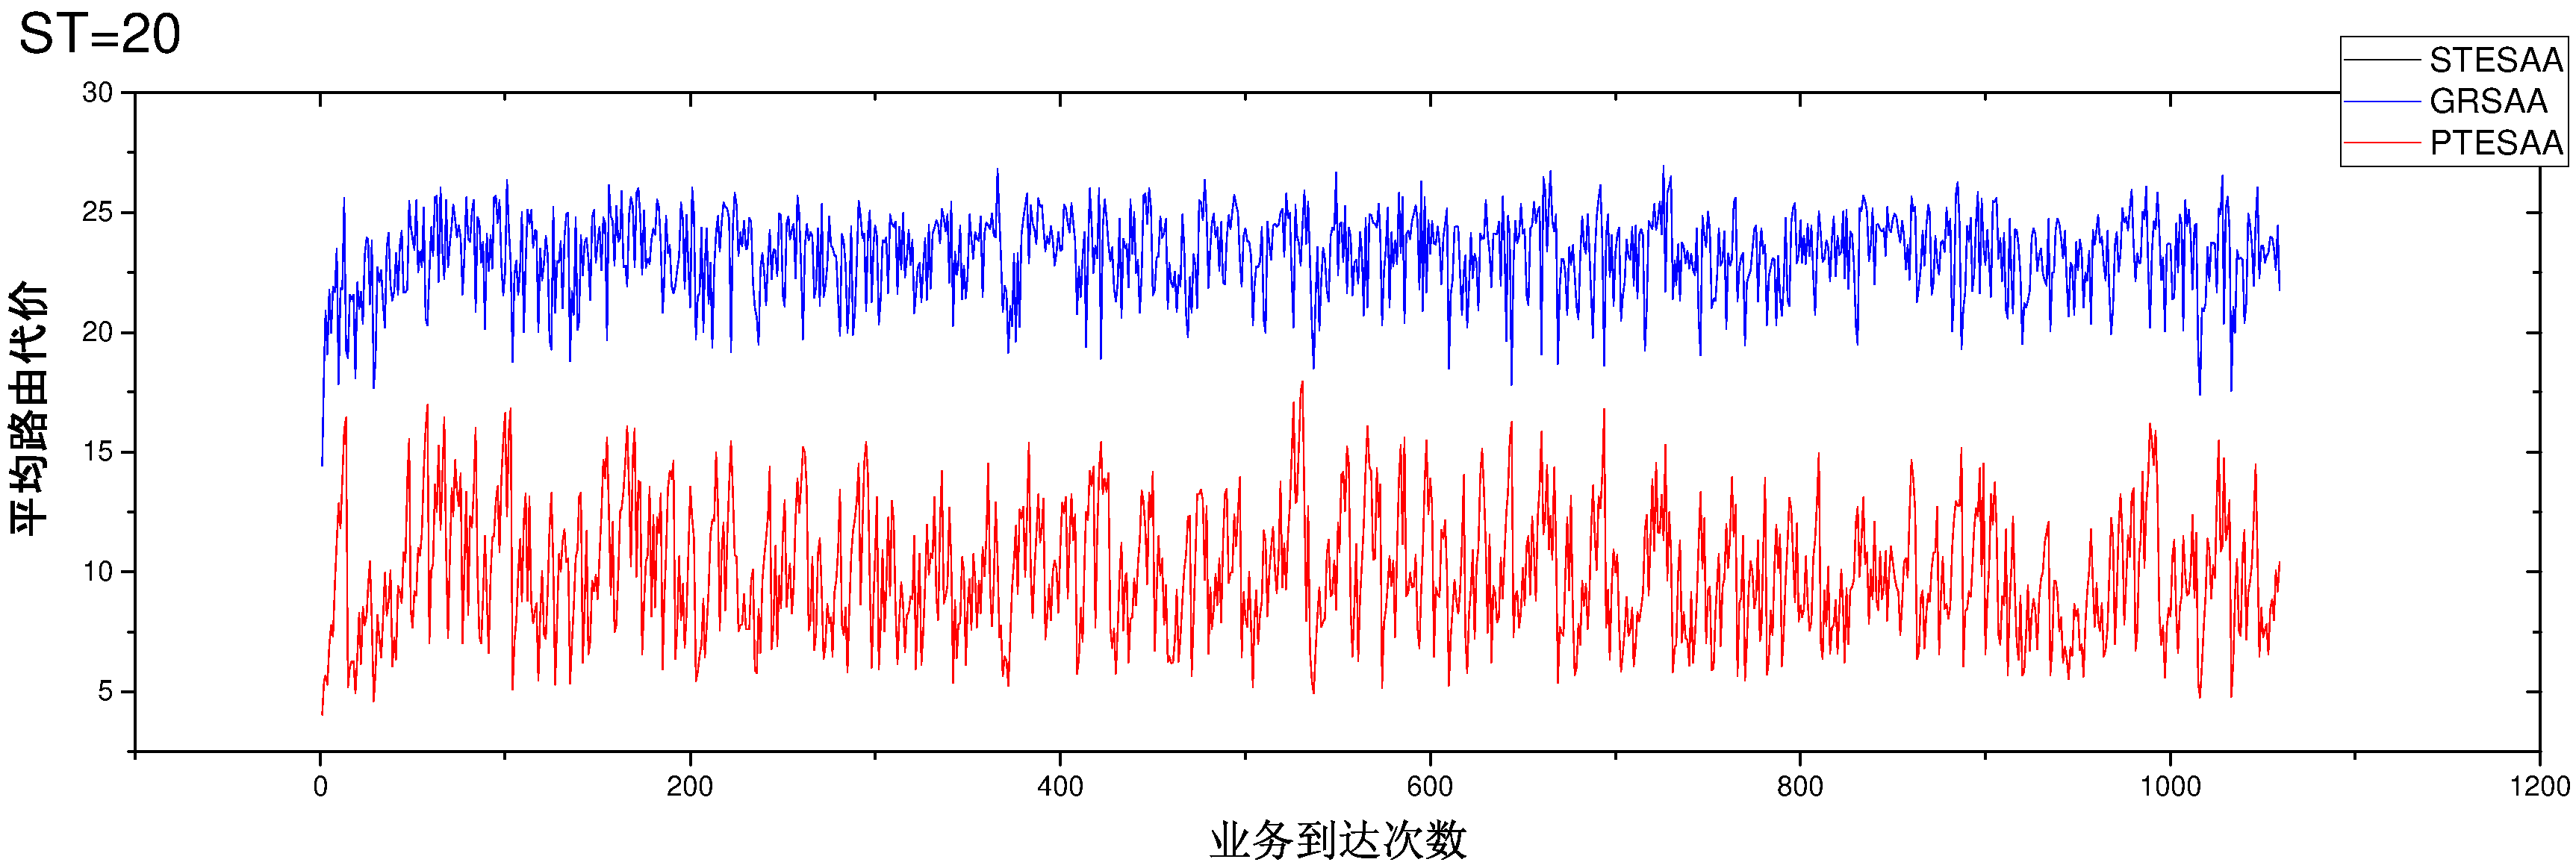
\includegraphics[width=1 \textwidth]{figures/H20C.pdf}}
\end{center}
\caption{{\footnotesize{带权图路由代价对比(ST=20)}}}
\label{H20C}
\end{figure*}
\begin{figure*}
\vspace{-0.5cm}
\setlength{\abovecaptionskip}{-0.5cm}
\begin{center}
{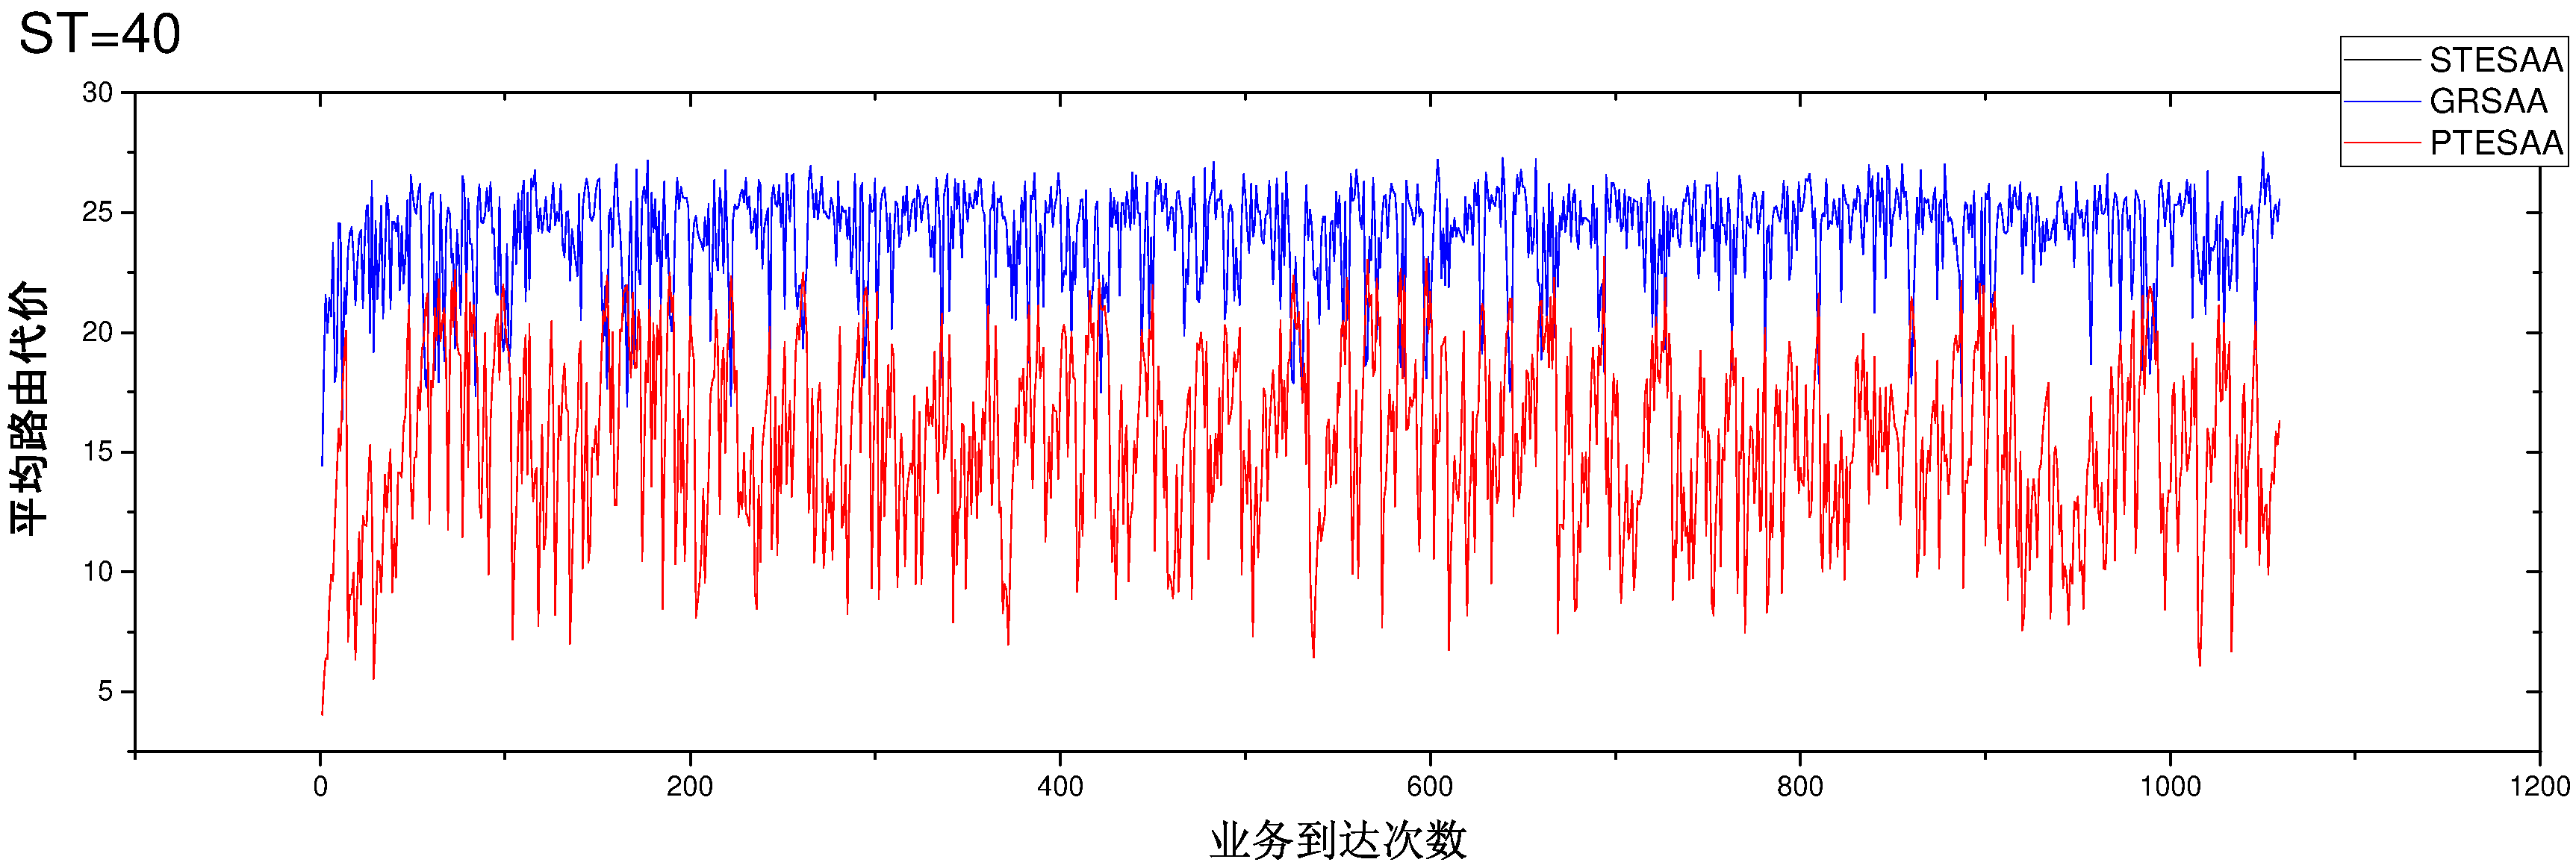
\includegraphics[width=1 \textwidth]{figures/H40C.pdf}}
\end{center}
\caption{{\footnotesize{带权图路由代价对比(ST=40)}}}
\label{H40C}
\end{figure*}
\begin{figure*}
\vspace{-0.5cm}
\setlength{\abovecaptionskip}{-0.5cm}
\begin{center}
{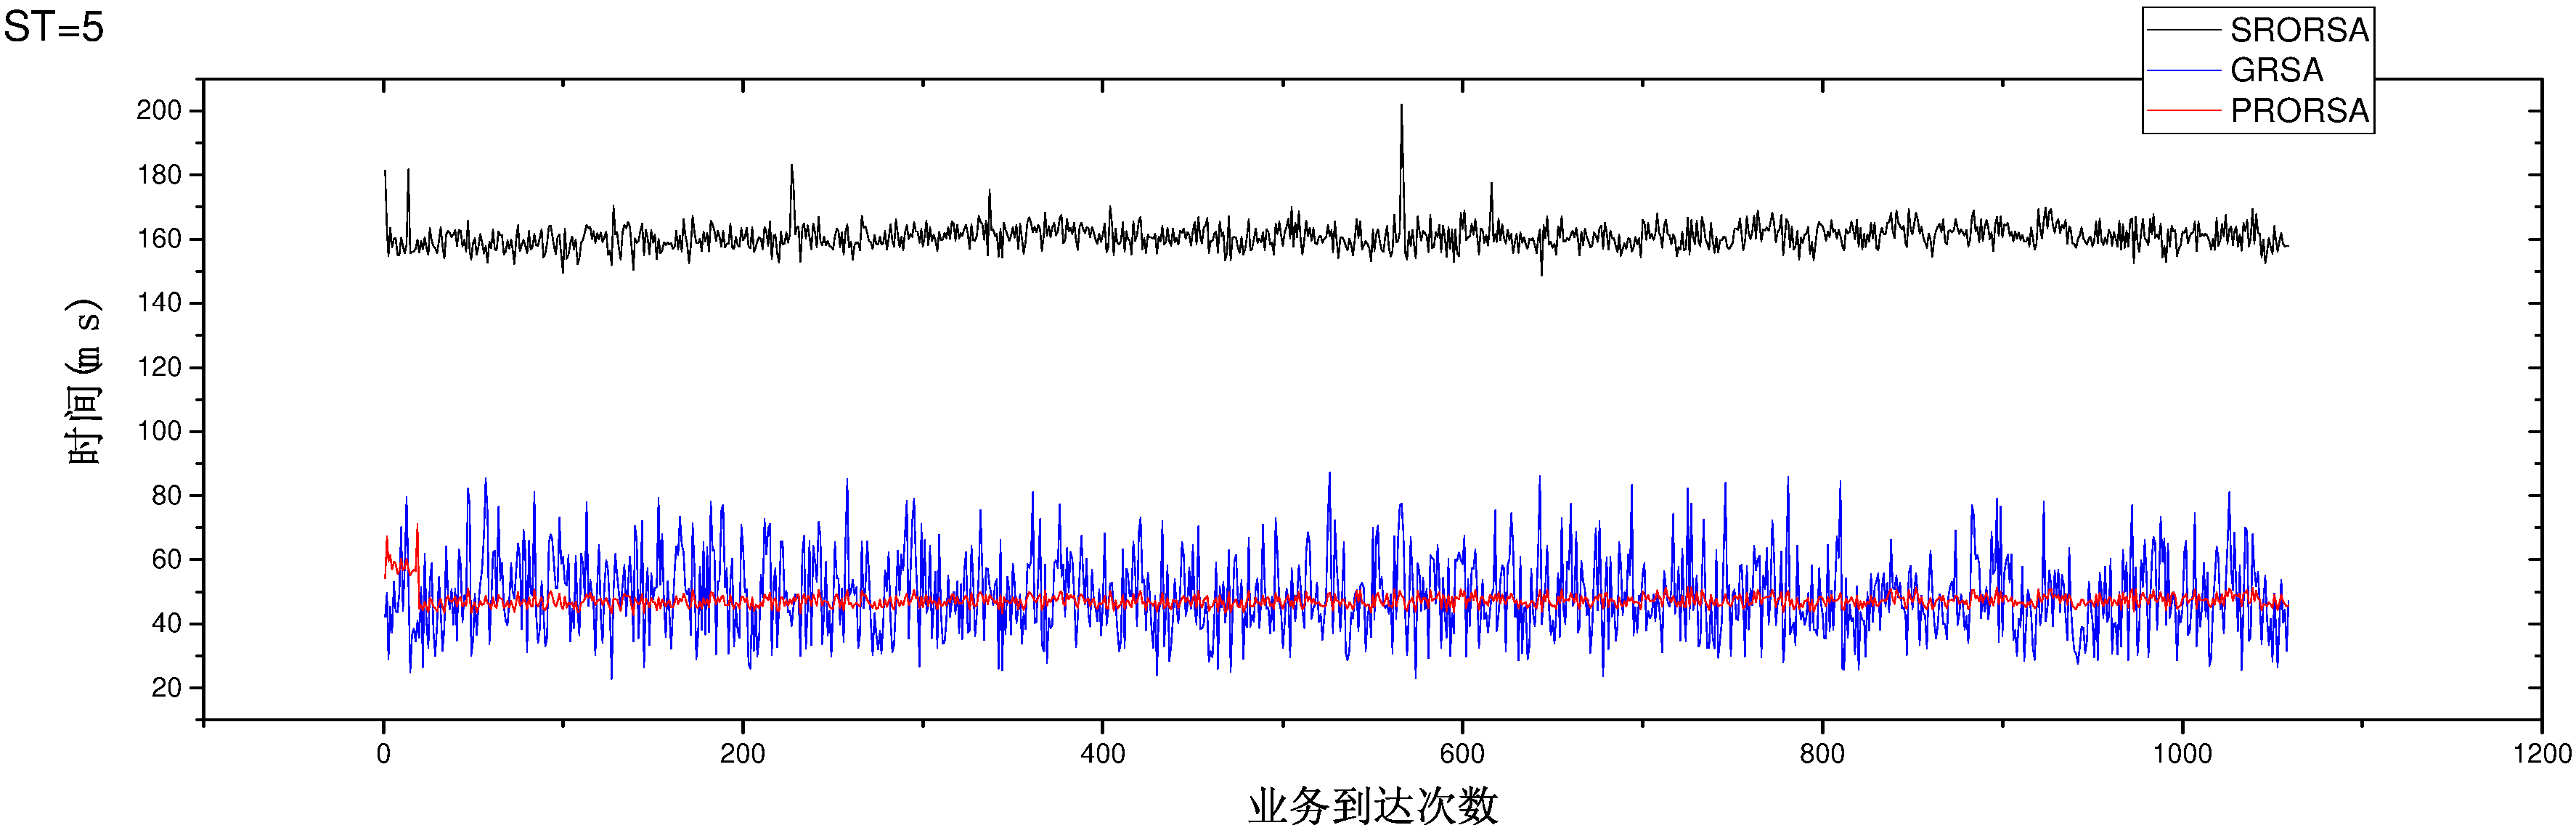
\includegraphics[width=1 \textwidth]{figures/H5T.pdf}}
\end{center}
\caption{{\footnotesize{带权图时间对比(ST=5)}}}
\label{H5T}
\end{figure*}
\begin{figure*}
\vspace{-0.5cm}
\setlength{\abovecaptionskip}{-0.5cm}
\begin{center}
{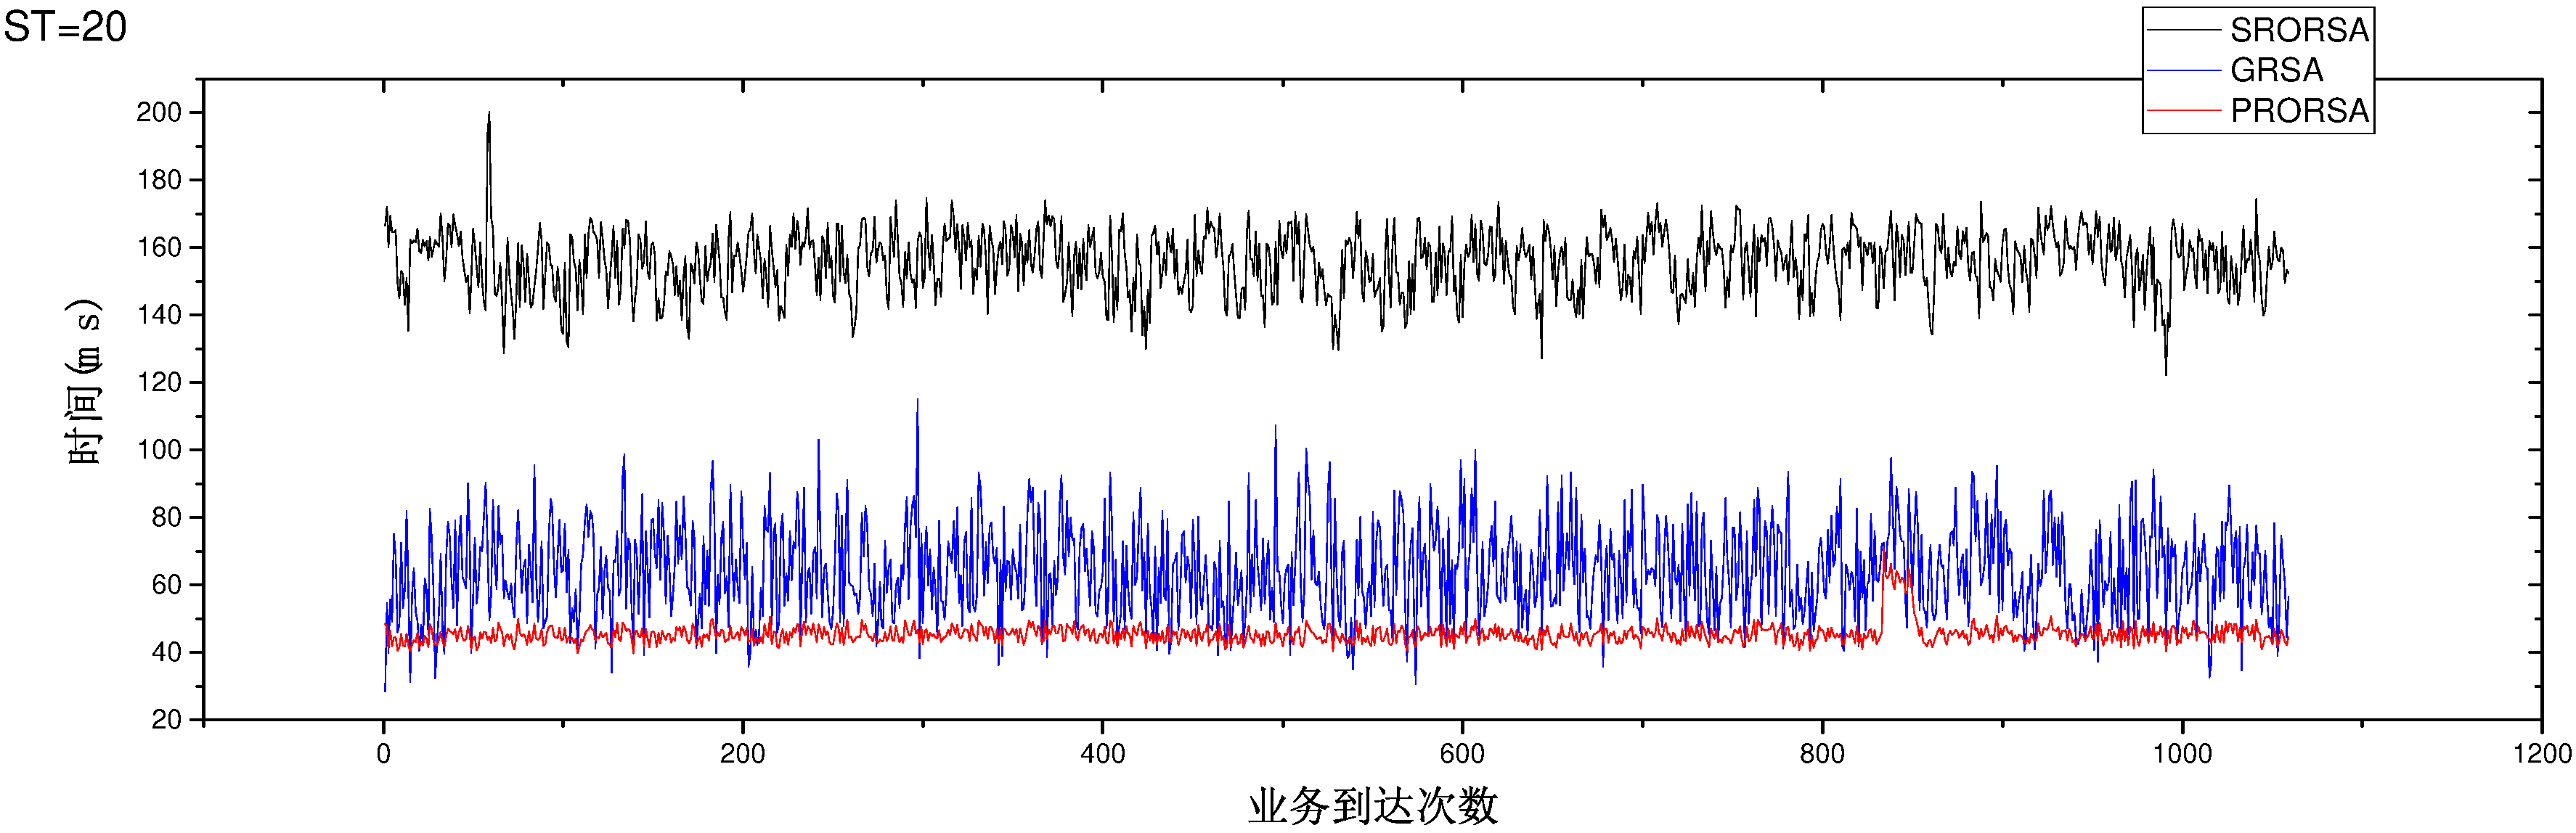
\includegraphics[width=1 \textwidth]{figures/H20T.pdf}}
\end{center}
\caption{{\footnotesize{带权图时间对比(ST=20)}}}
\label{H20T}
\end{figure*}
\begin{figure*}
\vspace{-0.5cm}
\setlength{\abovecaptionskip}{-0.5cm}
\begin{center}
\vspace{-0.1cm}
{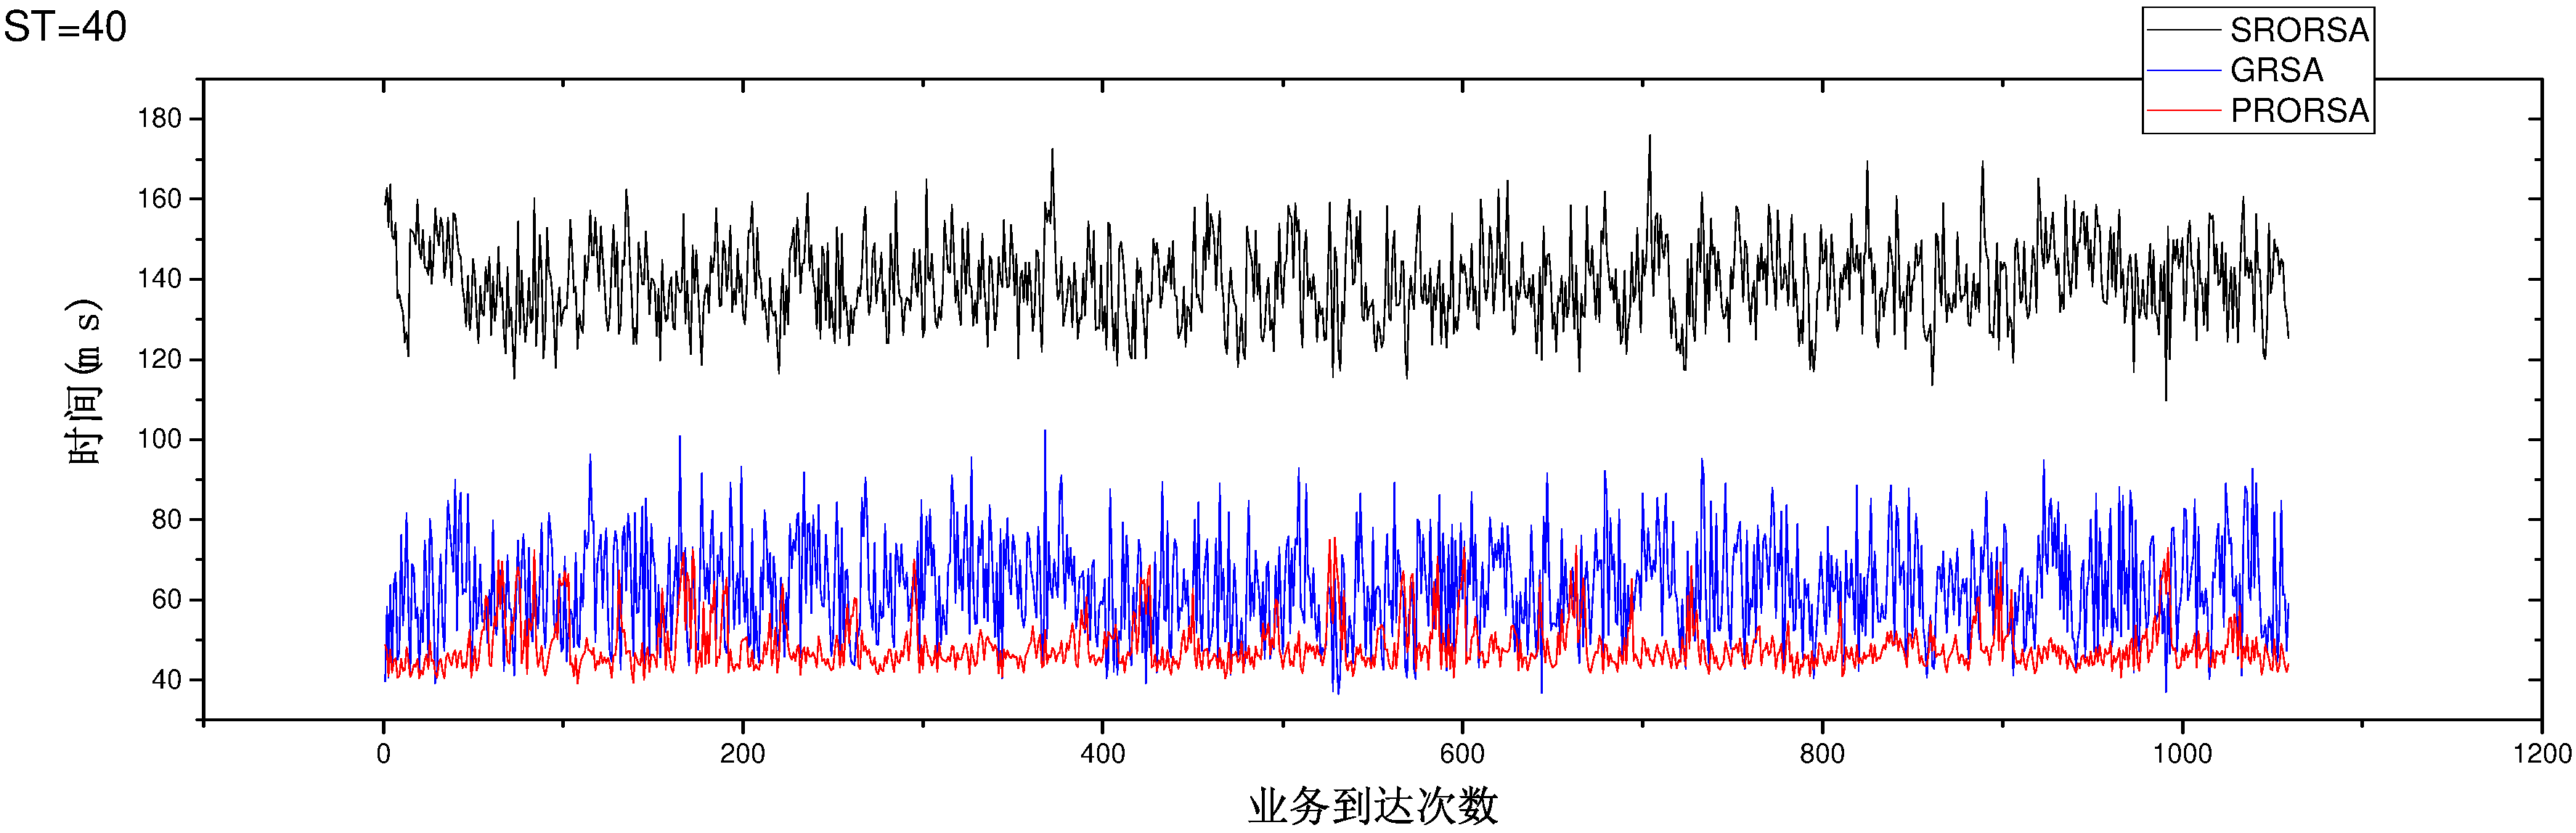
\includegraphics[width=1 \textwidth]{figures/H40T.pdf}}
\end{center}
\caption{{\footnotesize{带权图时间对比(ST=40)}}}
\label{H40T}
\end{figure*}
\begin{figure*}
\vspace{-0.1cm}
\setlength{\abovecaptionskip}{-0.5cm}
\begin{center}
{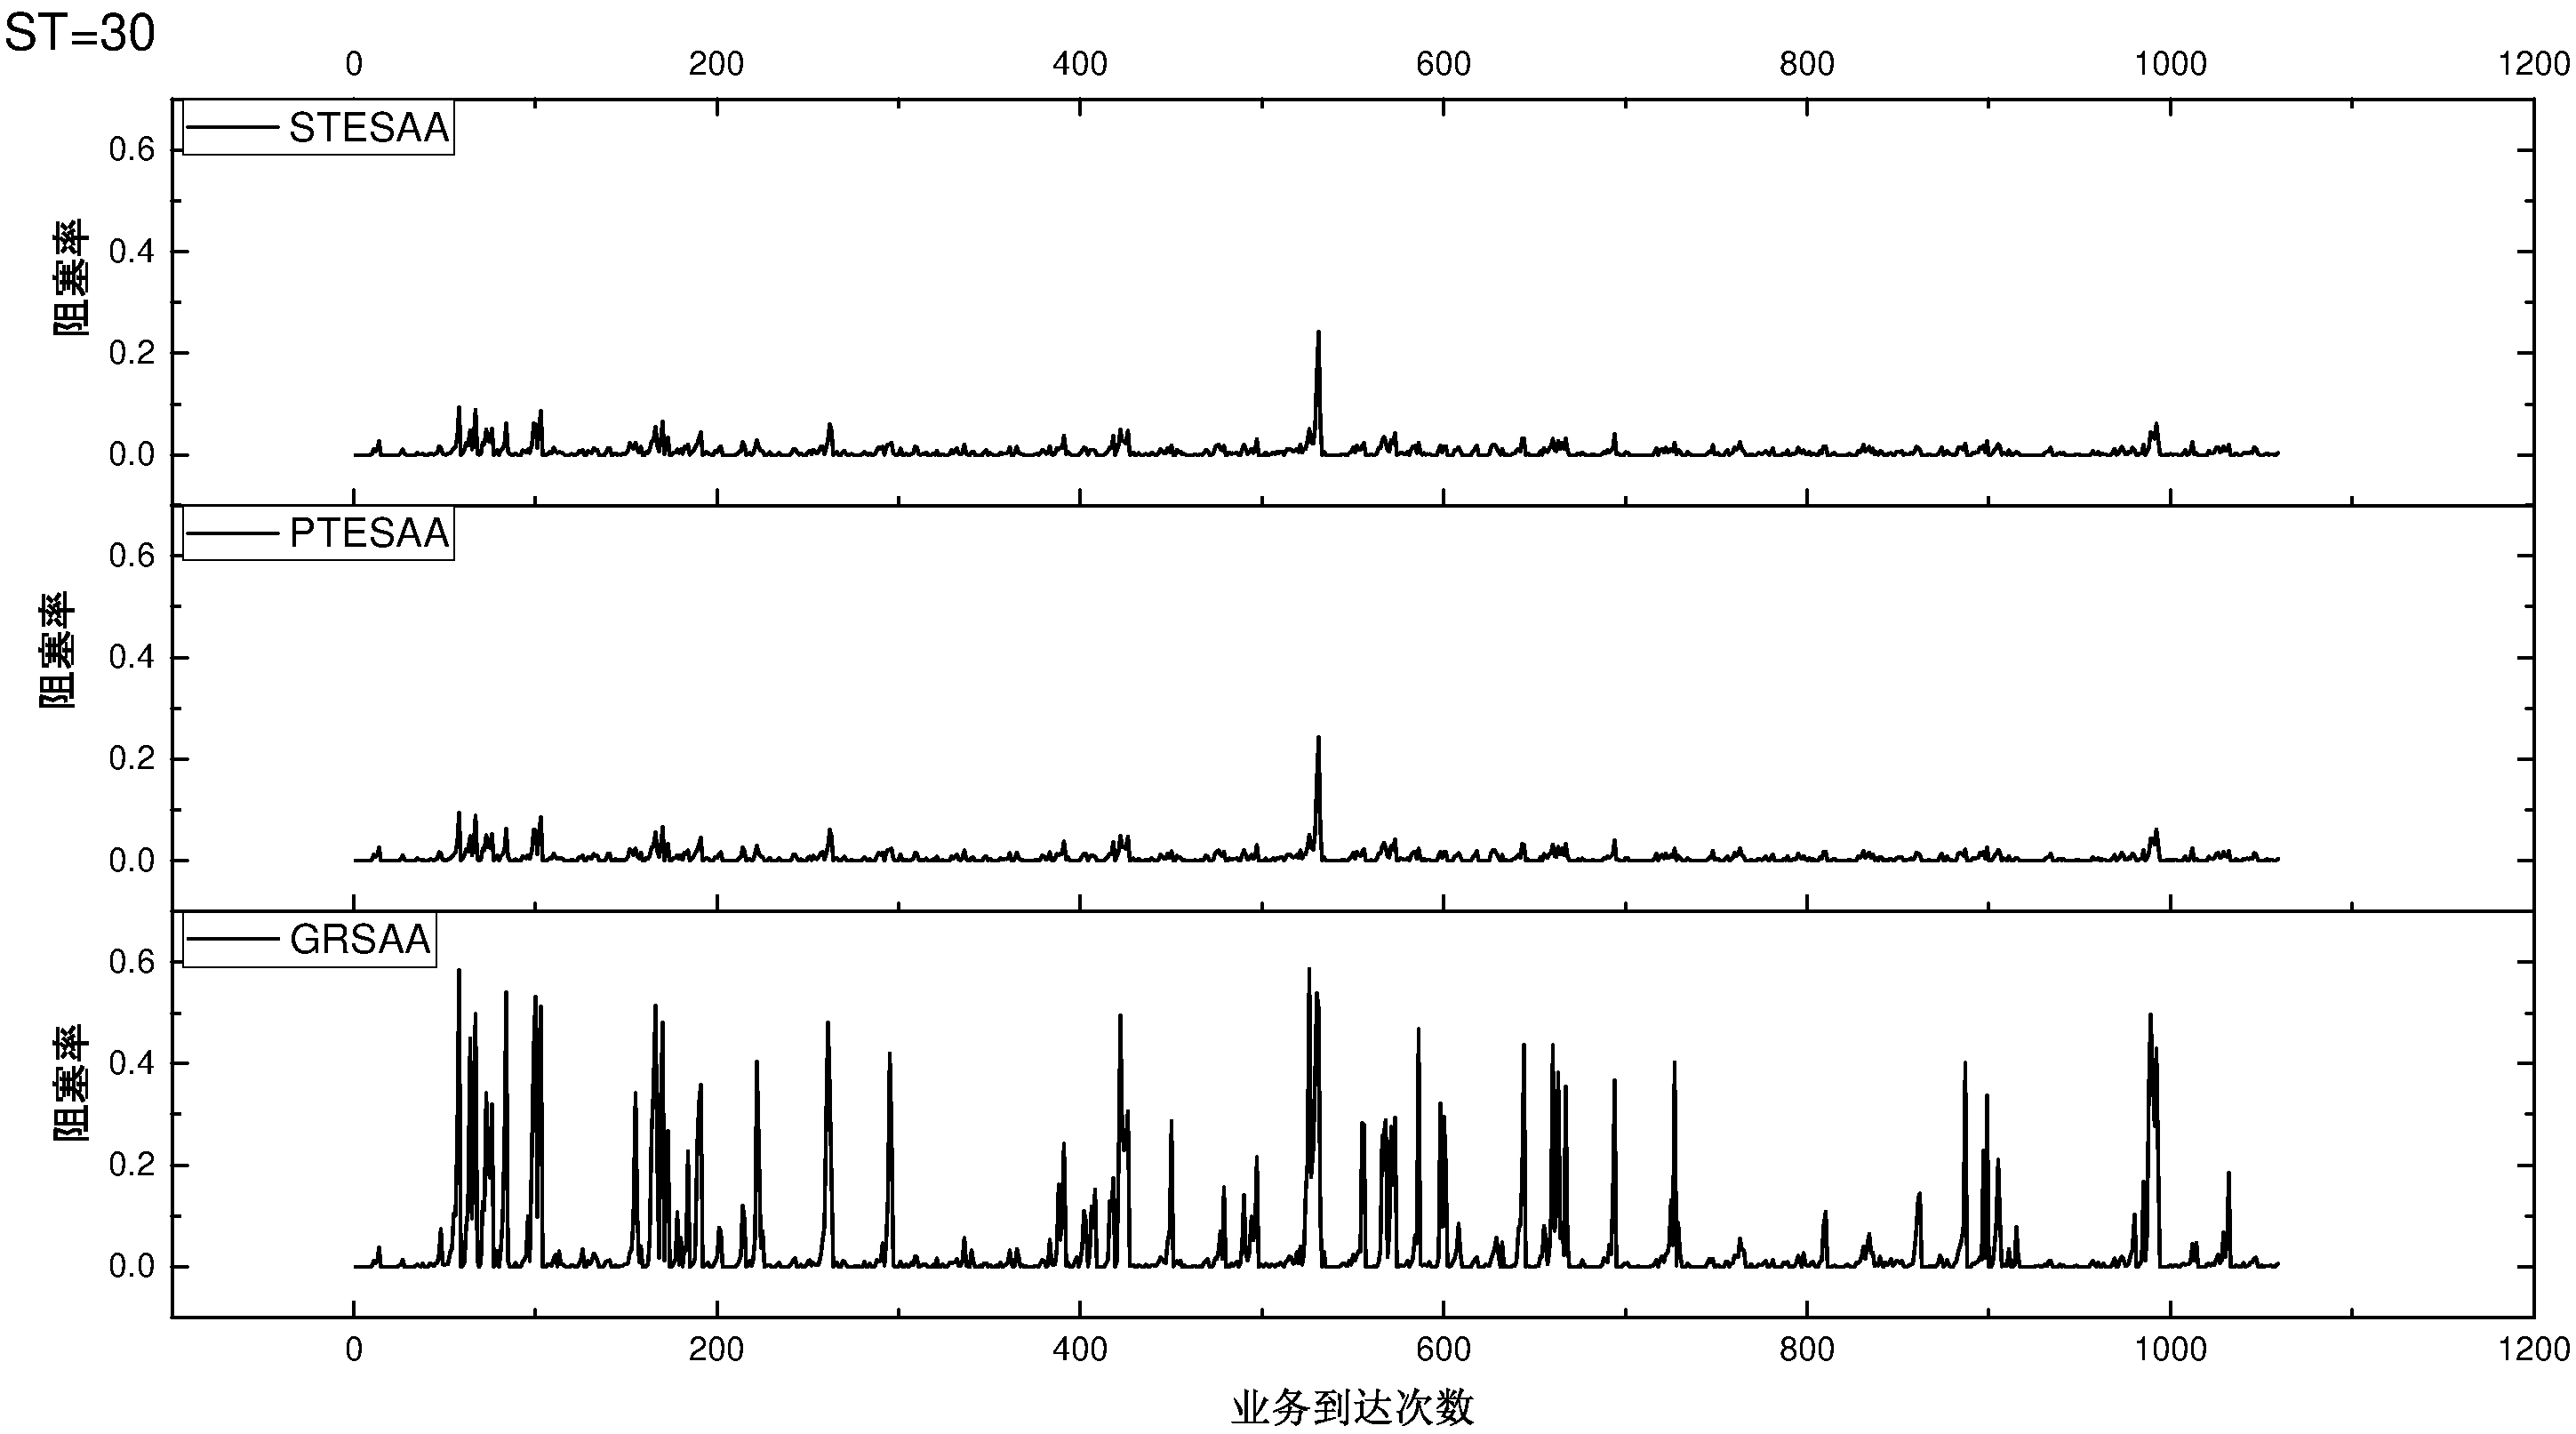
\includegraphics[width=0.8 \textwidth]{figures/H30Z.pdf}}
\end{center}
\caption{{\footnotesize{带权图阻塞率对比(ST=30)}}}
\label{H30Z}
\end{figure*}
\begin{figure*}
\setlength{\belowcaptionskip}{-0.5cm}
\begin{center}
{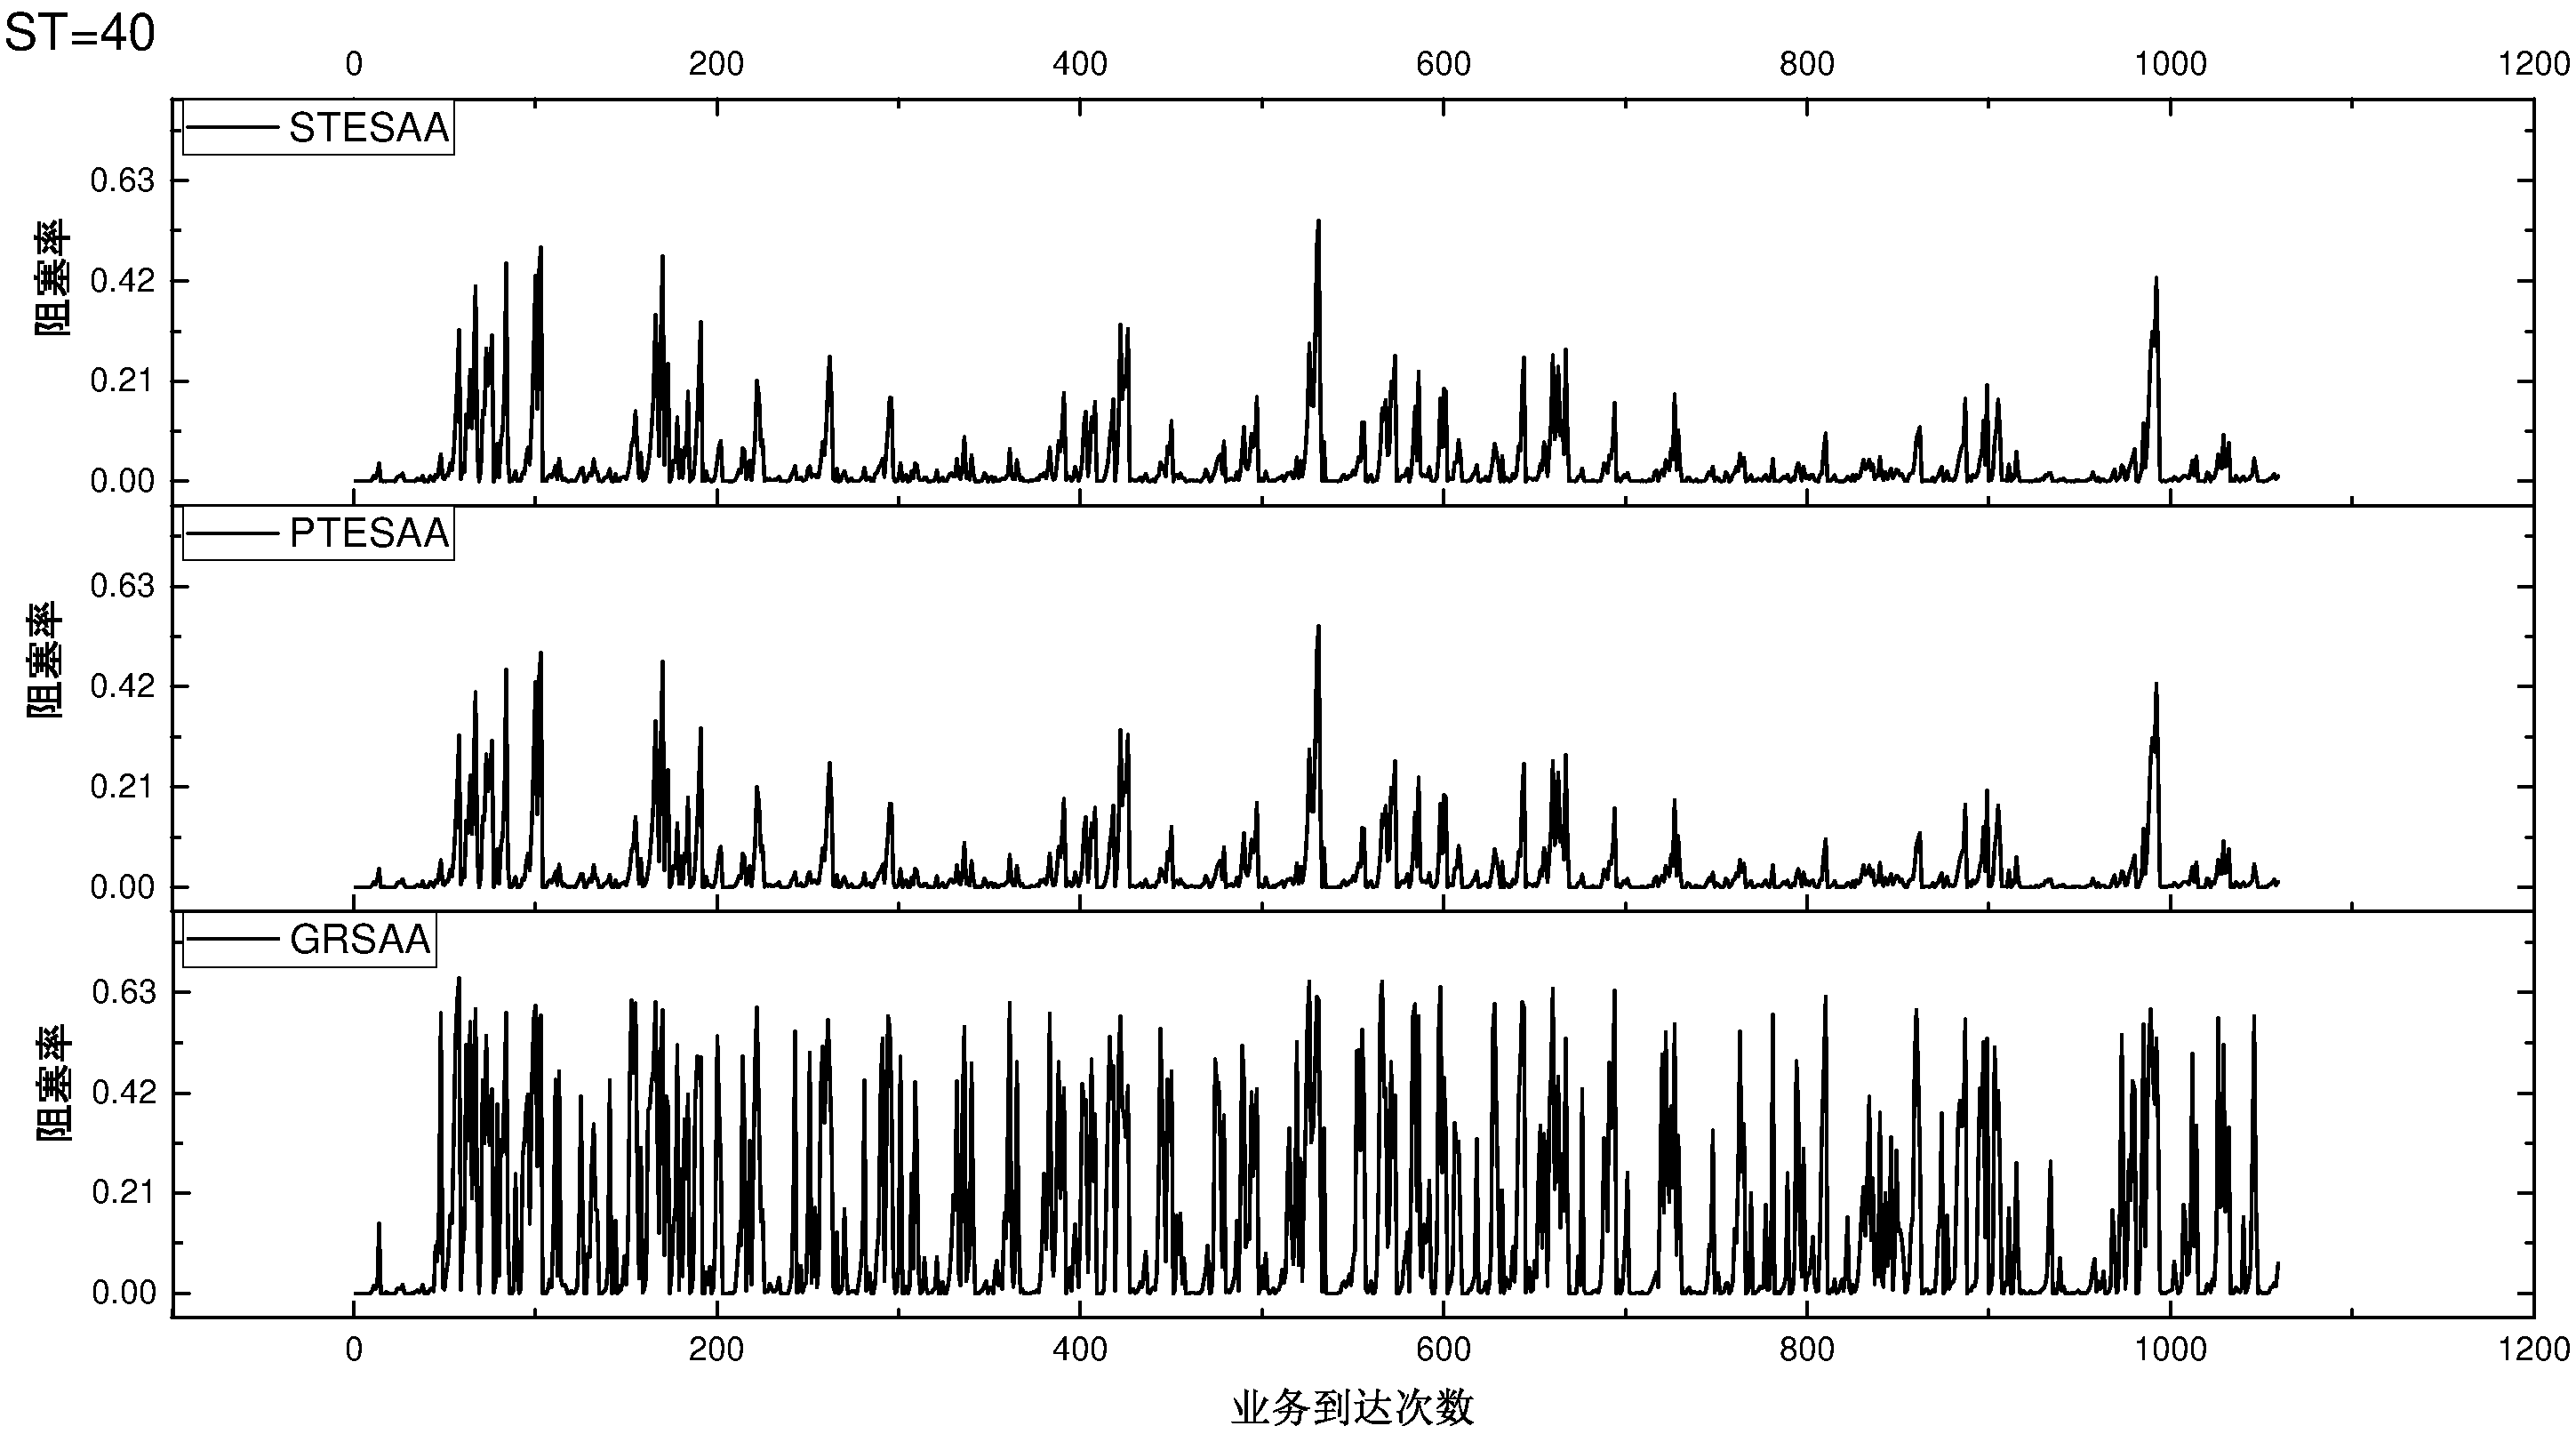
\includegraphics[width=0.8 \textwidth]{figures/H40Z.pdf}}
\end{center}
\caption{{\footnotesize{带权图阻塞率对比(ST=40)}}}
\label{H40Z}
\end{figure*}
带权图情况下我们把网络中每条链路的权值设置为1到10之间的随机整数值。图 \ref{H5C}和图 \ref{H40C}表示了路由代价的优化结果,我们把PTESAA和STESAA的优化结果与贪心算法GRSAA的结果进行比较,图中的横坐标表示业务到达的次数,纵坐标表示业务路由的平均代价。

当网络状况较好的时候,比如,平均服务时间为$ST=5$时,如图\ref{H5C}所示,算法PTESAA/STESAA得到的平均路由代价大约为GRSAA得到的平均路由代价的3到4分之一,路由代价得到很大优化。

当网络较拥塞时,比如,平均服务时间为$ST=40$时,如图\ref{H40C}所示,由于网络中的可用链路变少,业务的路径选择空间变小,使得业务可能会选择代价较大的路径进行路由,所以PTESAA/STESAA算法得到的平均路由代价变大,但是PTESAA/STESAA的平均路由代价依然比GRSAA的平均路由代价小很多。

\subsubsection{时间分析}
图 \ref{H5T}到图 \ref{H40T}展示了带权图中各个算法在不同平均服务时间$ST$下的计算时间,当$ST=5$时,我们可以看到PTESAA的计算时间是STESAA的计算时间的1/4,和无权图下PTESAA算法的计算一样,带权图下的PTESAA计算中步骤一的GPU加速比也可达到7-8倍,但是由于步骤二的计算时间不可忽略,使得总体加速比降为4-5倍。

观察图\ref{H5T}到图\ref{H40T},我们发现带权图下的PTESAA/STESAA的计算时间依然优于GRSAA的计算时间。另外,随着网络拥塞程度的增加,可用链路变少,PTESAA对STESAA的加速比略有下降。

\subsubsection{阻塞率分析}
虽然在带权图中,TESAA目标是去优化路由代价,而并不是去优化路由跳数,但是路由代价较小也在一定程度上意味着路由的跳数较小。所以在带权图中,PTESAA/STESAA求得的路径跳数也比较小,使用的链路资源较少,从而也能优化阻塞率。如图\ref{H30Z}和图\ref{H40Z}所示,带权图下的PTESAA/STESAA算法的阻塞率依然比GRSAA的阻塞率小很多。

\section{本章总结}
本章首先讨论了EON中的RSA问题,介绍了分层图模型,针对分层图模型设计了TESAA算法框架,对框架中路由计算部分进行了并行设计,分别在无权图和带权图两种情况下设计了基于GPU的并行算法,实验发现TESAA能够优化路径跳数,路径代价和阻塞率,同时,并行算法PTESAA对串行算法STESAA的加速比能达到5倍。
